% EcoExplain-VLM: study guide version 3 (20 October 2026).
% Personal learning material. Not for submission and not to be copied into the report.
% Compile:  latexmk -pdf ecoexplain_study_guide_v3.tex   (pdflatex + bibtex)
% Numbers:  python build_results_master.py   (writes chapters/generated_master_table.tex)
% Figures:  python make_figures_v3.py  and  python make_workflow_figure_corrected.py
\documentclass[11pt,a4paper,oneside]{report}

\usepackage[T1]{fontenc}
\usepackage[utf8]{inputenc}
\usepackage{lmodern}
\usepackage{microtype}
\usepackage[a4paper,margin=2.4cm]{geometry}
\usepackage{amsmath,amssymb}
\usepackage{booktabs,tabularx,longtable,multirow,makecell,array}
\newcolumntype{L}[1]{>{\raggedright\arraybackslash}p{#1}}
\newcolumntype{Y}{>{\raggedright\arraybackslash}X}
\usepackage{graphicx}
\usepackage{float}
\usepackage{caption}
\captionsetup{font=small,labelfont=bf}
\usepackage{xcolor}
\usepackage{enumitem}
\setlist{itemsep=2pt,topsep=4pt}
\usepackage[breakable,skins]{tcolorbox}
\usepackage{tikz}
\usetikzlibrary{arrows.meta,positioning}
\usepackage[hyphens]{url}
\usepackage[colorlinks=true,linkcolor=blue!50!black,citecolor=green!35!black,urlcolor=blue!60!black]{hyperref}
\usepackage[authoryear,round]{natbib}
\usepackage{fancyhdr}
\usepackage{titlesec}

\setlength{\parindent}{0pt}
\setlength{\emergencystretch}{3em}
\def\UrlBreaks{\do\/\do-\do\_\do.}
\setlength{\parskip}{5pt}
\renewcommand{\arraystretch}{1.18}

\titleformat{\chapter}[display]{\normalfont\bfseries\Large}{\chaptertitlename\ \thechapter}{8pt}{\huge}
\titlespacing*{\chapter}{0pt}{-10pt}{18pt}

\pagestyle{fancy}
\fancyhf{}
\fancyhead[R]{\footnotesize\nouppercase{\leftmark}}
\fancyfoot[C]{\thepage}

% ---------- boxes ----------
\definecolor{plainc}{RGB}{33,97,140}
\definecolor{whyc}{RGB}{30,120,70}
\definecolor{watchc}{RGB}{176,58,46}
\definecolor{reportc}{RGB}{110,60,140}
\definecolor{codec}{RGB}{90,90,90}
\definecolor{newc}{RGB}{196,120,20}
\definecolor{checkc}{RGB}{20,120,130}
\newtcolorbox{plainwords}{breakable,colback=plainc!5,colframe=plainc,fonttitle=\bfseries\small,title=In plain words}
\newtcolorbox{whybox}{breakable,colback=whyc!5,colframe=whyc,fonttitle=\bfseries\small,title=Why it was done this way}
\newtcolorbox{watchout}{breakable,colback=watchc!5,colframe=watchc,fonttitle=\bfseries\small,title=Watch out}
\newtcolorbox{foryourreport}{breakable,colback=reportc!5,colframe=reportc,fonttitle=\bfseries\small,title=For your own report}
\newtcolorbox{wherecode}{breakable,colback=codec!4,colframe=codec,fonttitle=\bfseries\small,title=Where it lives in the project}
\newtcolorbox{newinfo}{breakable,colback=newc!6,colframe=newc,fonttitle=\bfseries\small,title=New or corrected in this version}
\newtcolorbox{selfcheck}{breakable,colback=checkc!5,colframe=checkc,fonttitle=\bfseries\small,title=Check yourself (answers in Appendix~\ref{app:answers})}

% ---------- shortcuts ----------
\newcommand{\file}[1]{\nolinkurl{#1}}
\newcommand{\dndvi}{\ensuremath{\Delta}NDVI}
\newcommand{\dnbr}{\ensuremath{\Delta}NBR}
\newcommand{\degC}{\ensuremath{^{\circ}}C}
\newcommand{\dg}{\ensuremath{^{\circ}}}

\begin{document}

\begin{titlepage}
\centering
\vspace*{2.2cm}
{\Huge\bfseries EcoExplain-VLM\par}
\vspace{0.5cm}
{\LARGE Study guide, version 3\par}
\vspace{0.3cm}
{\large Learn the whole project from the beginning,\\ then correct and rewrite your report yourself\par}
\vspace{1.4cm}
{\large Forest change in Kanha Tiger Reserve $\cdot$ five satellite and climate sources\\
four open vision--language models $\cdot$ classification, fine-tuning and explanations\par}
\vspace{1.4cm}
\begin{tcolorbox}[colback=watchc!5,colframe=watchc,width=0.86\textwidth]
\small This guide is study material. It explains every part of the project so that you can write your own report in your own words. It is not a manuscript: do not submit it or copy sentences from it. Every number in it was read from a file in the project, and the file is named next to the number so that you can check it yourself.
\end{tcolorbox}
\vspace{0.8cm}
\begin{tcolorbox}[colback=newc!6,colframe=newc,width=0.86\textwidth]
\small \textbf{Version 3.} Everything in version~2, updated with the leak-free reruns of 19--20 October: Qwen and LLaVA without the summary line, the balanced class LoRA (Ada job 29575), the parser fix and the spatial split. One chapter now holds every result, recomputed from the files.
\end{tcolorbox}
\vfill
{\large 20 October 2026\par}
\end{titlepage}

\tableofcontents

\part{Start here}
\chapter{How to use this guide}
\label{ch:start}

\section{Who this guide is for}

You built EcoExplain-VLM over about four months, and now you have to explain it in a report that your professor will read closely. This guide assumes you are starting from zero. It explains every idea the project uses, shows exactly what was done at each step, gives every result with the file it came from, and then helps you check and rewrite your own draft.

The guide follows your own workflow figure (Figure~\ref{fig:workflow-yours} in Chapter~\ref{ch:bigpicture}). That figure has five stages, numbered 01 to 05. Part~II of the guide has one chapter for each of the first four stages, Part~III explains the models and the scoring you need for stage~05, and Part~IV covers the three evaluation tracks of stage~05 one by one.

\section{What is in each part}

\begin{description}[style=nextline,leftmargin=1.2cm]
  \item[Part I. Start here (Chapters 1--3)] How to read the guide; the whole project on a few pages (the workflow figure explained box by box, the order in which the work happened, the numbers to know by heart); and every result in one table.
  \item[Part II. The workflow, stage by stage (Chapters 4--7)] Stage~01, the five data sources, with the remote-sensing ideas behind them. Stage~02, Earth Engine and image processing. Stage~03, how the labels and the evidence cards were made. Stage~04, the frozen dataset and the train/development/test split.
  \item[Part III. Models and measurement (Chapters 8--9)] What a vision--language model is, the four models used and exactly what each one received, LoRA fine-tuning, and every metric used to score classifications and explanations.
  \item[Part IV. The three evaluation tracks (Chapters 10--12)] Track~A, zero-shot classification. Track~B, class LoRA. Track~C, explanations (free-form, structured, and the explanation LoRA). Each chapter gives the results, how to read them, and what they do not show.
  \item[Part V. Putting it together (Chapter 13)] The answer to the research question, the hypotheses, the objectives, the limitations and the future work.
  \item[Part VI. From understanding to your report (Chapters 14--17)] A check of every figure you have; a section-by-section review of your current draft; a writing plan with word budgets and the references that fit each section; and the questions your professor is likely to ask.
  \item[Appendices] Every key number with its source file, a map of the project folders, a glossary, and the answers to the self-check questions.
\end{description}

\section{A reading plan}

You do not have to read the guide in one go. A plan that works in about a week:

\begin{table}[H]
\centering
\small
\begin{tabular}{lL{6.4cm}L{6.0cm}}
\toprule
Day & Read & Then do this \\
\midrule
1 & Chapters 1--3 & Draw the workflow figure from memory, with the key numbers. \\
2 & Chapters 4--5 (stages 01--02) & Explain NDVI, SAR backscatter and median compositing aloud in two minutes each. \\
3 & Chapters 6--7 (stages 03--04) & Open \file{dataset.jsonl}, find one test patch, and read its evidence card. \\
4 & Chapters 8--9 & Write the LoRA equation and the Wilson interval from memory. \\
5 & Chapters 10--12 & Re-create the main results table on paper and say what each row means. \\
6 & Chapters 13--14 & List the limitations in your own words; decide which figures go in the report. \\
7 & Chapters 15--17 & Go through the draft review and fix your draft, section by section. \\
\bottomrule
\end{tabular}
\end{table}

Each chapter ends with a ``Check yourself'' box. Answer the questions without looking back, then compare with Appendix~\ref{app:answers}. If you can answer them, you can defend that part of the report.

\section{The boxes}

Seven kinds of box appear in the guide.

\begin{plainwords}
A short explanation without jargon.
\end{plainwords}
\begin{whybox}
The reason a choice was made, and what the alternatives were.
\end{whybox}
\begin{watchout}
A problem, inconsistency or trap. These matter most for an honest report.
\end{watchout}
\begin{foryourreport}
What this means for the report you will write. These boxes list what to include. They never contain finished report sentences: the sentences must be yours.
\end{foryourreport}
\begin{wherecode}
The files, functions and notebook cells that implement the idea, so you can check it.
\end{wherecode}
\begin{newinfo}
Something that was added or corrected since an earlier version of the guide (version~1: 6 October; version~2: 19 October 2026). Read these boxes first if you know an earlier version.
\end{newinfo}
\begin{selfcheck}
Questions to test your understanding at the end of each chapter.
\end{selfcheck}

\section{Conventions}

\begin{itemize}
  \item File paths are relative to the project folder \file{ecoexplain_vlm_dataset/} unless they start with \file{ada_review/} (files copied back from the IIIT Ada cluster), \file{report/} or \file{study_guide_v2/} (folders next to the project folder).
  \item Percentages are on the 55 test patches unless stated otherwise.
  \item ``Gold'' or ``label'' always means \texttt{candidate\_class}, the automatic label used for all scoring.
  \item \textbf{Phases} are the order in which the work happened (A, B, C, D). \textbf{Tracks} are the three experiments in stage~05 of your workflow figure (A, B, C). The letters do not mean the same thing; Table~\ref{tab:phasetrack} in Chapter~\ref{ch:bigpicture} maps one onto the other.
\end{itemize}

\section{What changed in version 3}

Version~2 (19 October) added the explanation LoRA, the exact input of each model, a check of your figures and a review of your draft. On 19--20 October you then fixed several protocol problems in the code and re-ran the key experiments. Version~3 brings those results in and corrects what they overturn.

\begin{newinfo}
\begin{enumerate}
  \item \textbf{One chapter with every result} (Chapter~\ref{ch:results}), recomputed from the prediction files by \file{build_results_master.py}. Its table is generated, so it cannot drift from the files.
  \item \textbf{Leak-free zero-shot results} (Chapter~\ref{ch:trackA}). Without the summary line Qwen2-VL-2B scores 32.7\,\% (\texttt{evidence\_only}) and 32.7\,\% (\texttt{compact}, answering ``stable'' for every patch); LLaVA-Interleave-0.5B scores 43.6\,\% (\texttt{compact}). PaliGemma could not be loaded and BLIP-2 gave no parsable answer.
  \item \textbf{A correction of version~2.} Version~2 said Qwen ``did not copy the label'' because it followed the card's trend words. Those trend words appear \emph{only} in the summary line, next to \texttt{candidate\_class}. Qwen did not copy the label token, but it did depend on that line; without it, it falls to chance (Chapter~\ref{ch:trackA}).
  \item \textbf{The balanced, leak-free class LoRA} (Ada job 29575; Chapter~\ref{ch:trackB}): 16 patches (6 decline, 5 stable, 5 increase), label-free card at training and test, 36.4\,\%. It answers ``stable'' for 53 of 55 patches. The old 67.3\,\% run is superseded.
  \item \textbf{Code changes} you made (Chapters~\ref{ch:stage04} and~\ref{ch:models}): the \texttt{compact} text mode that gives every model the same table, the parser that ignores echoed prompts, \texttt{--balanced-train}, and a spatial block split (266/46/54).
  \item \textbf{GitHub.} The code, the new results and a README section (4.7) are on the \texttt{main} branch of \texttt{Rama-Vaibhav/EcoExplain-VLM} (Appendix~\ref{app:files}).
  \item \textbf{The draft review} (Chapter~\ref{ch:draft}) now says which issues you report as fixed and adds the checks the new results require.
\end{enumerate}
\end{newinfo}

The version~2 changes (Phase~D, unequal model inputs, the first-16-by-ID training sets, the real LLaVA checkpoint, the raster-based card text, the two score files) are all still in the guide where they belong.

\section{A promise about numbers}

Every number in this guide was read from a project file or recomputed from one, and the source is named. Where the project does not record something (for example, why the candidate pool has an empty strip), the guide says so instead of guessing. When you write your report, keep to the same rule: if you cannot point to the file a number came from, do not use the number.

\chapter{The whole project in one picture}
\label{ch:bigpicture}

\section{The project in five sentences}

\begin{enumerate}
  \item You built a benchmark of \textbf{366 forest patches} (each about 640\,m across) in the Kanha Tiger Reserve region of Madhya Pradesh, each seen in two matched dry seasons: \textbf{T0 = January--February 2022} and \textbf{T1 = January--February 2023}.
  \item For every patch you collected \textbf{five data sources} (Sentinel-2 optical, Sentinel-1 radar, CHIRPS rainfall, ERA5-Land climate anomalies, NASADEM terrain), made a before/after pair of colour images and a text \textbf{evidence card}, and gave it an automatic label: \texttt{decline}, \texttt{stable} or \texttt{increase}, from the change in NDVI.
  \item You tested \textbf{four small open vision--language models} on the same 55 test patches. With the full card, whose last line states the label, Qwen2-VL-2B reached \textbf{56.4\,\%} and the other three 32.7--36.4\,\%. With that line removed, Qwen fell to \textbf{32.7\,\%} and LLaVA reached 43.6\,\%: no model beats always guessing one class (34.5\,\%).
  \item A small \textbf{LoRA fine-tune} of Qwen2-VL-2B on 16 balanced training patches with the label-free card reached \textbf{36.4\,\%}, answering ``stable'' for almost everything. An earlier, unbalanced run with the full card (67.3\,\%) is superseded.
  \item When the models had to \textbf{justify} their answers with the label removed, free-form text was unreliable; a \textbf{structured ``cite-only'' prompt} made 71--76\,\% of checkable claims agree with the measurements, and a pilot \textbf{explanation LoRA} on 16 self-generated justifications reached 61.8\,\% class accuracy but only 50.5\,\% correct claims.
\end{enumerate}

\section{The research question and what kind of project this is}

The research roadmap (\file{EcoExplain-VLM_Complete_Research_Roadmap.pdf}, Section~1) states the central question:

\begin{quote}
\emph{Can vision--language models correctly classify forest vegetation change and generate explanations that are supported by multimodal remote-sensing and climate evidence?}
\end{quote}

The question has two halves, and the project has two halves to match: \textbf{classification} (Tracks~A and~B) and \textbf{explanation} (Track~C).

\begin{plainwords}
EcoExplain-VLM is an \emph{evaluation benchmark}, not a new remote-sensing model. You did not try to beat existing forest-change maps. You built a fixed test, put existing general-purpose models through it, and measured carefully what they could and could not do. A clear negative or mixed result is a valid outcome for a benchmark, as long as it is measured honestly.
\end{plainwords}

\section{Your workflow figure, box by box}

Figure~\ref{fig:workflow-yours} is the workflow figure you made for your report (\file{papers/acl/fig_workflow.png}). It is the map for the whole guide: each numbered stage has its own chapter.

\begin{figure}[H]
\centering
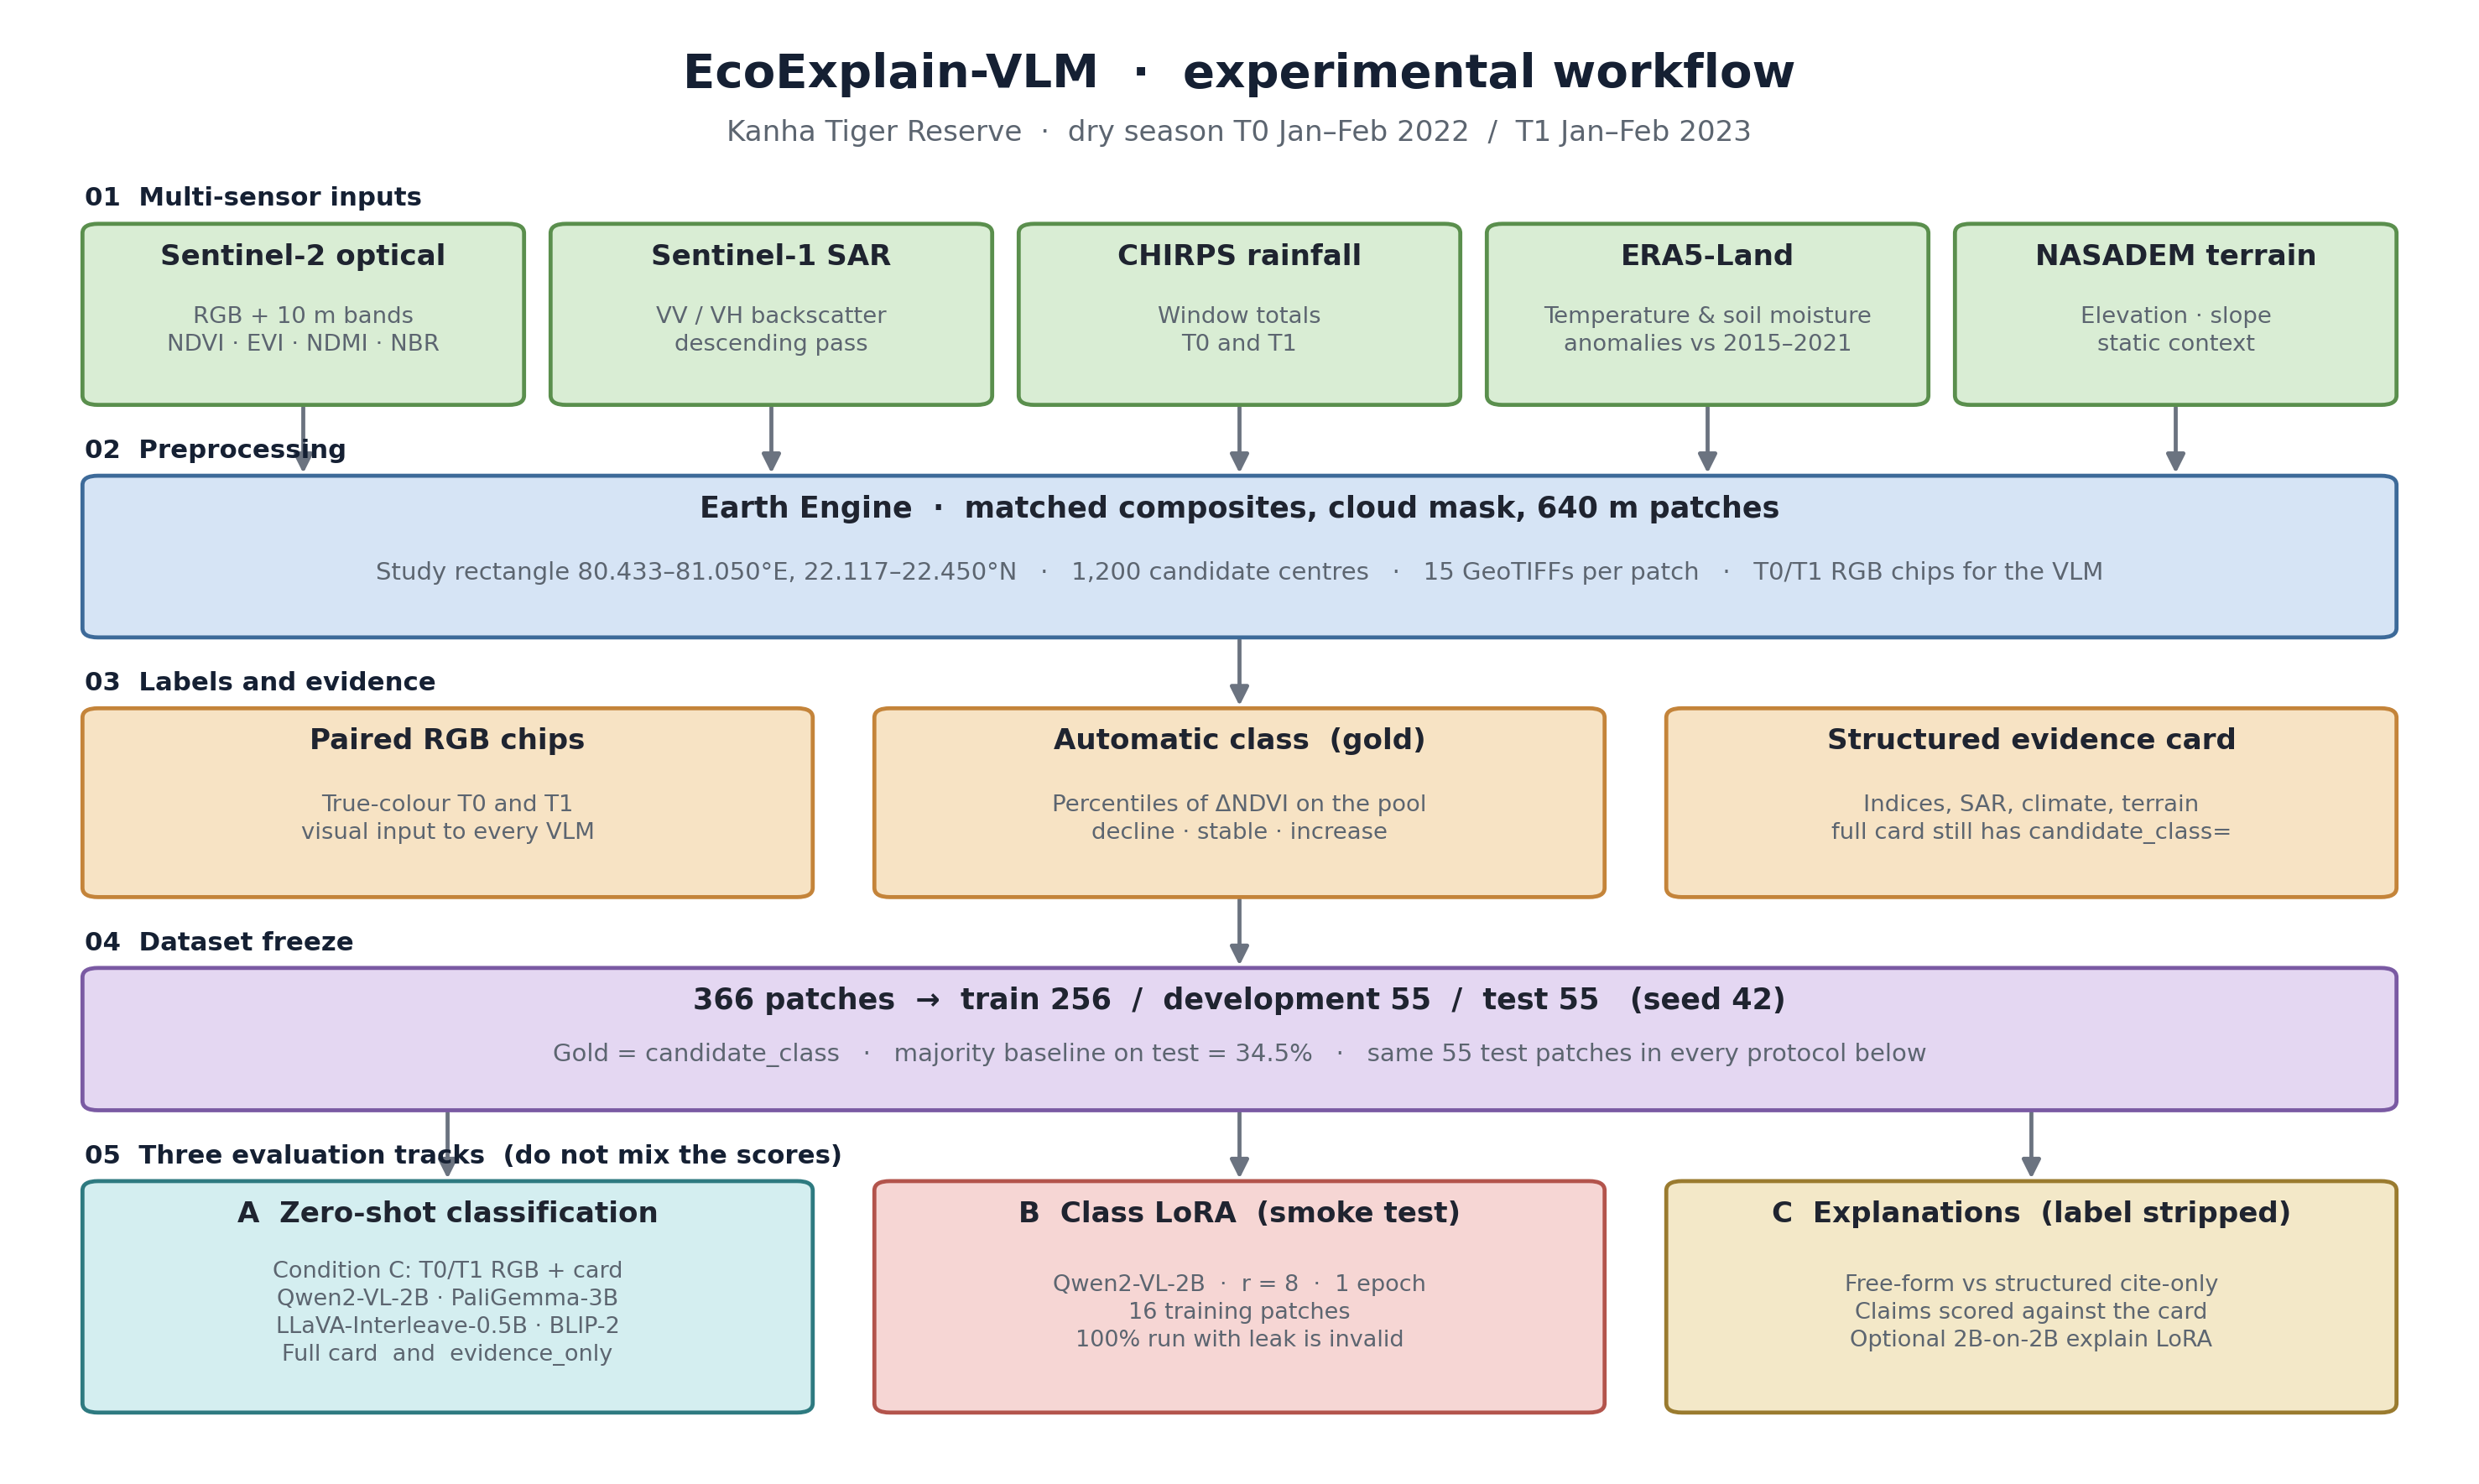
\includegraphics[width=\textwidth]{figures/fig_workflow_yours.png}
\caption{Your workflow figure, as it is now (\file{papers/acl/fig_workflow.png}, made by \file{papers/acl/make_workflow_figure.py}). Two box texts in stage~05 need correcting; Chapter~\ref{ch:figures} explains why and shows a corrected copy.}
\label{fig:workflow-yours}
\end{figure}

\begin{longtable}{L{2.6cm}L{8.2cm}L{3.0cm}}
\caption{What each stage of the workflow means, and where the guide explains it.}\label{tab:stages}\\
\toprule
\textbf{Stage} & \textbf{What happens} & \textbf{Guide} \\
\midrule
\endfirsthead
\toprule
\textbf{Stage} & \textbf{What happens} & \textbf{Guide} \\
\midrule
\endhead
01 Multi-sensor inputs & Five sources describe each place: what the canopy looks like and how green it is (Sentinel-2), its structure and wetness (Sentinel-1), rain (CHIRPS), temperature and soil moisture compared with normal (ERA5-Land), and terrain (NASADEM). & Chapter~\ref{ch:stage01} \\
02 Preprocessing & Google Earth Engine combines all images of each two-month window into one cloud-free picture per year, cuts 640\,m patches around candidate centres, and exports 15 files per patch. Image processing then makes 512\,$\times$\,512 colour chips and arrays. & Chapter~\ref{ch:stage02} \\
03 Labels and evidence & Three things come out for every patch: a pair of colour images (T0, T1), an automatic label from the NDVI change, and a text evidence card listing the measured values. & Chapter~\ref{ch:stage03} \\
04 Dataset freeze & The 366 records are frozen in \file{dataset.jsonl} and split once into 256 training, 55 development and 55 test patches. Always predicting the most common test class scores 34.5\,\%. & Chapter~\ref{ch:stage04} \\
05 Three evaluation tracks & A: four models classify the test patches without training. B: one model is fine-tuned with LoRA and tested again. C: the models are asked to justify their answers, and their claims are checked against the measurements. & Chapters~\ref{ch:trackA}--\ref{ch:trackC} \\
\bottomrule
\end{longtable}

\begin{watchout}
Two things in the figure are not accurate, and both matter because the figure will be one of the first things your professor looks at:
\begin{itemize}
  \item Track~A says every model received ``T0/T1 RGB + card''. Only Qwen2-VL-2B and LLaVA-Interleave-0.5B did. PaliGemma received one NDVI line, and BLIP-2 one stitched image with no evidence text.
  \item Track~A lists ``Full card and evidence\_only'' as if all four models were run both ways. The \texttt{evidence\_only} re-run covered three models on all 55 patches and Qwen on only 3, and it changed the input of LLaVA only.
\end{itemize}
Chapter~\ref{ch:figures} gives the exact lines to change in \file{make_workflow_figure.py} and a corrected copy.
\end{watchout}

\section{The order in which the work happened: four phases}

The work did not happen in the neat order of the figure. It happened in four phases, each prompted by what the previous one showed (Figure~\ref{fig:phases}).

\begin{figure}[H]
\centering
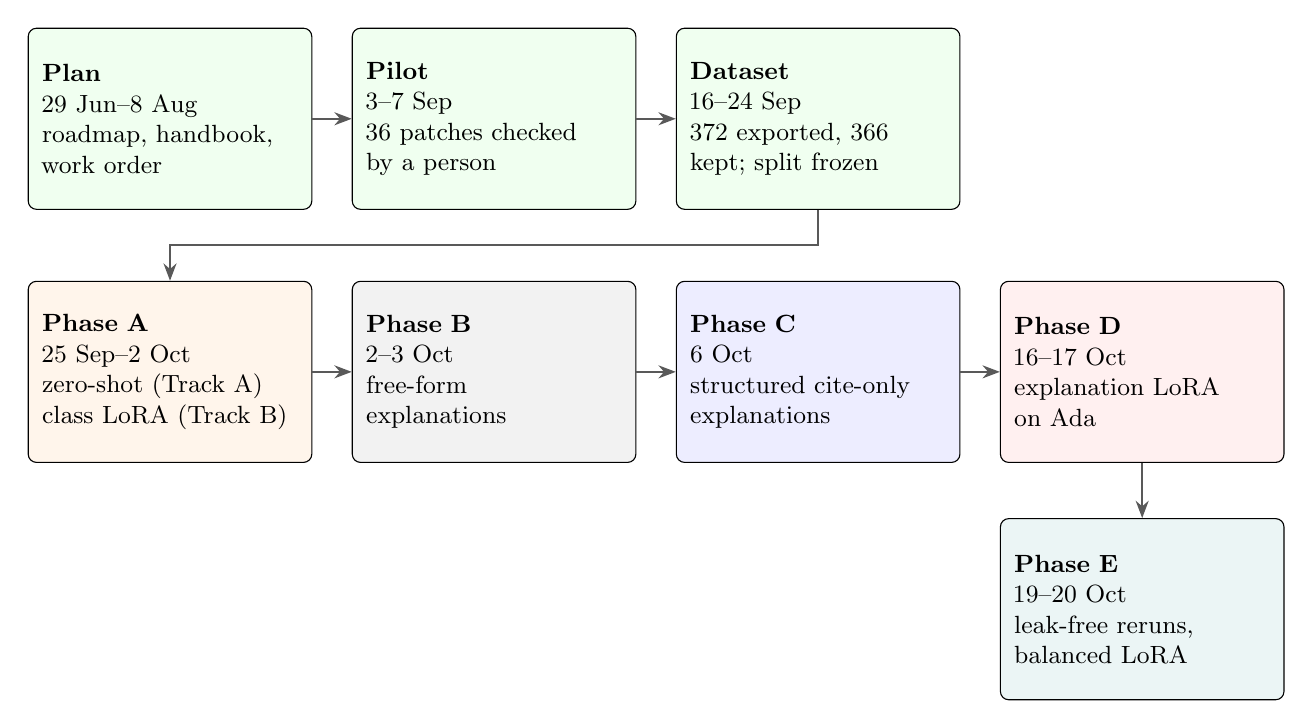
\begin{tikzpicture}[
  box/.style={draw, rounded corners=3pt, align=left, font=\small, inner sep=5pt, text width=3.25cm, minimum height=2.3cm},
  prep/.style={box, fill=green!6},
  pha/.style={box, fill=orange!8},
  phb/.style={box, fill=gray!10},
  phc/.style={box, fill=blue!7},
  phd/.style={box, fill=red!6},
  arr/.style={-{Stealth[length=2.2mm]}, thick, gray!70!black}
]
\node[prep] (plan) {\textbf{Plan}\\ 29 Jun--8 Aug\\ roadmap, handbook,\\ work order};
\node[prep, right=0.5cm of plan] (pilot) {\textbf{Pilot}\\ 3--7 Sep\\ 36 patches checked\\ by a person};
\node[prep, right=0.5cm of pilot] (data) {\textbf{Dataset}\\ 16--24 Sep\\ 372 exported, 366\\ kept; split frozen};
\node[pha, below=0.9cm of plan] (A) {\textbf{Phase A}\\ 25 Sep--2 Oct\\ zero-shot (Track A)\\ class LoRA (Track B)};
\node[phb, right=0.5cm of A] (B) {\textbf{Phase B}\\ 2--3 Oct\\ free-form\\ explanations};
\node[phc, right=0.5cm of B] (C) {\textbf{Phase C}\\ 6 Oct\\ structured cite-only\\ explanations};
\node[phd, right=0.5cm of C] (D) {\textbf{Phase D}\\ 16--17 Oct\\ explanation LoRA\\ on Ada};
\node[box, fill=teal!8, below=0.7cm of D] (E) {\textbf{Phase E}\\ 19--20 Oct\\ leak-free reruns,\\ balanced LoRA};
\draw[arr] (plan) -- (pilot);
\draw[arr] (pilot) -- (data);
\draw[arr] (data.south) -- ++(0,-0.45) -| (A.north);
\draw[arr] (A) -- (B);
\draw[arr] (B) -- (C);
\draw[arr] (C) -- (D);
\draw[arr] (D) -- (E);
\end{tikzpicture}
\caption{The order of the work in 2026. Dates come from file times, notebook outputs, Slurm logs and the git history; the first guide (\file{study_guide/}, Chapter~3) has the day-by-day timeline.}
\label{fig:phases}
\end{figure}

\begin{table}[H]
\centering
\caption{Phases (when the work happened) against tracks (how your workflow figure groups the experiments).}
\label{tab:phasetrack}
\small
\begin{tabularx}{\textwidth}{lYY}
\toprule
Phase & What it did & Track in your figure \\
\midrule
A & Four models classify the 55 test patches; Qwen2-VL-2B fine-tuned with LoRA on 16 patches; supporting runs (label line removed, closed-set probe, threshold baselines) & Track~A (zero-shot) and Track~B (class LoRA) \\
B & Models asked to explain their answer in their own words (``free-form'' or ``legacy'' prompt) & Track~C, first part \\
C & Models asked to copy listed facts and follow a stated rule (``structured cite-only'' prompt) & Track~C, second part \\
D & Qwen2-VL-2B fine-tuned on 16 of its own filtered explanations (``explanation LoRA'') & Track~C, third part \\
E & Protocol fixes and reruns: Qwen and LLaVA without the summary line; balanced, label-free class LoRA; parser fix; spatial split & Track~A (leak-free rows) and Track~B (new run) \\
\bottomrule
\end{tabularx}
\end{table}

\begin{foryourreport}
Pick one naming scheme for the report and keep to it. The tracks of your figure are the clearer choice for a Methods section, because they describe experiments rather than dates. If you keep the letters A/B/C for tracks, do not also call the explanation prompts ``Phase B'' and ``Phase C'' in the same report, or a reader will confuse Track~B (class LoRA) with Phase~B (free-form explanations). Descriptive names avoid the problem: ``zero-shot classification'', ``class LoRA'', ``free-form explanations'', ``structured explanations'', ``explanation LoRA''.
\end{foryourreport}

\section{What was found, in one paragraph per track}

\paragraph{Track A, zero-shot classification.} With the full card, Qwen2-VL-2B was correct on 31 of 55 test patches (56.4\,\%); PaliGemma-3B scored 36.4\,\%, LLaVA-Interleave-0.5B and BLIP-2 OPT-2.7B 32.7\,\% each, the level of always predicting one class (the majority baseline is 34.5\,\%). Removing the summary line dropped Qwen to 32.7\,\% (a significant drop, $p = 0.011$), and with the same label-free table for every model LLaVA reached 43.6\,\% (not significantly above the baseline). A one-number rule on the evidence card's \dndvi{} value, with two cut-offs fitted on the training split, scores 94.5\,\%: the card holds enough information, but the small models do not extract it.

\paragraph{Track B, class LoRA.} The reported run (Ada job 29575) fine-tuned Qwen2-VL-2B on 16 class-balanced training patches with the label-free card, for one epoch: 36.4\,\% (20 of 55), answering ``stable'' for 53 patches. The first run (16 patches chosen by ID, full card) reached 67.3\,\% but read the card's label line and never answered ``stable''; longer full-card runs reached 100\,\%. Both are superseded.

\paragraph{Track C, explanations.} With a free-form prompt, PaliGemma and BLIP-2 gave no checkable reasons and LLaVA's claims were right 56.7\,\% of the time. A structured prompt that lists allowed facts and states an NDVI rule raised claim correctness to 75.8\,\% (Qwen) and 71.1\,\% (LLaVA), but the answers mostly restate the given facts, and Qwen's class simply follows the stated rule. The explanation LoRA reached 61.8\,\% class accuracy with 50.5\,\% correct claims, worse on claims than structured prompting.

\section{The numbers to know by heart}

\begin{longtable}{L{6.0cm}L{3.0cm}L{5.2cm}}
\caption{Twelve numbers that carry the report. Appendix~\ref{app:facts} has the full list.}\label{tab:heart}\\
\toprule
\textbf{Quantity} & \textbf{Value} & \textbf{Source file} \\
\midrule
\endfirsthead
\toprule
\textbf{Quantity} & \textbf{Value} & \textbf{Source file} \\
\midrule
\endhead
Study rectangle & 80.433--81.050\dg E, 22.117--22.450\dg N; 2,350.7\,km$^2$ & \file{configs/pilot_kanha.yaml}; notebook 01 \\
Windows & T0 Jan--Feb 2022; T1 Jan--Feb 2023 & \file{configs/pilot_kanha.yaml} \\
Patches & 1,200 candidates $\rightarrow$ 366 final (120 / 124 / 122) & \file{data/raw_metadata/composite_stats.csv}, \file{dataset.jsonl} \\
Label cut-offs & $q_{15} = -0.0377$, $q_{85} = +0.0031$ & computed from the 1,200-patch pool \\
Split & 256 / 55 / 55, seed 42; test 18 / 18 / 19 & \file{data/splits/split_manifest.json} \\
Majority baseline & 34.5\,\% (19/55) & same \\
Human check & 8 of 19 agree (42\,\%) & \file{results/preflight_report.json} \\
Zero-shot, full card (Track A) & Qwen 56.4\,\%; PaliGemma 36.4\,\%; LLaVA 32.7\,\%; BLIP-2 32.7\,\% & \file{results/vlm_combo_*.json} \\
Zero-shot, leak-free (Track A) & Qwen 32.7\,\% (\texttt{evidence\_only} and \texttt{compact}); LLaVA 43.6\,\% (\texttt{compact}) & \file{results/protocol/} \\
Class LoRA (Track B) & 36.4\,\% (balanced 16, label-free, Ada job 29575); old 67.3\,\% superseded & \file{results/protocol/qwen_balanced_leakfree_lora.json} \\
Threshold baseline & 94.5\,\% (fitted on train); 63.6\,\% ($\pm0.02$) & \file{study_guide_v3/build_results_master.py} \\
Structured explanations & 75.8\,\% (Qwen), 71.1\,\% (LLaVA) correct claims & \file{results/explain/explanation_scores.csv} \\
Explanation LoRA & 61.8\,\% class accuracy; 50.5\,\% correct claims; 28/256 kept, 16 used & \file{results/explain/explanation_scores.json}, \file{target_filter_report.json} \\
\bottomrule
\end{longtable}

\section{Five things the report must say clearly}

These five statements protect the whole report. An examiner who finds any of them missing will doubt the rest.

\begin{enumerate}
  \item \textbf{What the full card contains.} Every evidence card ends with the pipeline's summary line, which includes the trend word and \texttt{candidate\_class}, the same field used as the gold label. Qwen's 56.4\,\% (and the old 67.3\,\%) were obtained with that card (Chapter~\ref{ch:trackA}).
  \item \textbf{What happens without it.} Qwen falls to 32.7\,\%; no model beats the 34.5\,\% baseline without the line. This is now your central classification finding, not a footnote.
  \item \textbf{What each model received.} Qwen and LLaVA: both images and the full card. PaliGemma: both images and one NDVI line. BLIP-2: one stitched image and a short prompt (Table~\ref{tab:inputs}).
  \item \textbf{How small the fine-tunes were.} Every LoRA run reported used 16 training examples for one epoch. Say this every time 36.4\,\% or 61.8\,\% appears.
  \item \textbf{What the labels are.} Relative ranks of NDVI change inside this region and pair of years, checked by one person on 19 patches with 42\,\% agreement. They are not a validated map of forest disturbance.
\end{enumerate}

\begin{whybox}
Stating these does not weaken the report; it fixes what the numbers mean. ``Qwen2-VL-2B reached 56.4\,\% with the full card and 32.7\,\% without its summary line'' is a clear, honest finding about what small VLMs actually use. Reporting 56.4\,\% alone would turn a true number into a misleading one.
\end{whybox}

\begin{selfcheck}
\begin{enumerate}
  \item In one sentence each, what happens in stages 01, 02, 03, 04 and 05 of your workflow?
  \item What is the difference between Phase~B and Track~B?
  \item Why is 34.5\,\%, and not 33.3\,\%, the number to compare models against?
  \item Which two models saw the full evidence card in Track~A?
  \item Name the five things the report must say clearly.
\end{enumerate}
\end{selfcheck}

\chapter{All results in one place}
\label{ch:results}

This chapter holds every score of the project in one table, recomputed from the saved prediction files. Use it as your reference while writing; the chapters after it explain where each number comes from and what it means.

\begin{wherecode}
\file{study_guide_v3/build_results_master.py} reads the result files under \file{ecoexplain_vlm_dataset/results/} and writes three things: \file{RESULTS_MASTER.md} (open it in any editor), \file{RESULTS_MASTER.json}, and \file{chapters/generated_master_table.tex}, the table below. After any new run, execute it again and rebuild this PDF; the table then cannot disagree with the files.
\end{wherecode}

\begin{watchout}
Rows in different sections of Table~\ref{tab:master} used different inputs. Never rank or average them without naming the input. The most common mistake is to put 56.4\,\% (full card, label line present) next to 32.7\,\% (label line removed) as if they were two models.
\end{watchout}

% Generated by build_results_master.py. Do not edit by hand.
\begingroup\small
\begin{longtable}{L{1.9cm}L{3.7cm}L{3.4cm}L{2.7cm}L{1.6cm}}
\caption{Every classification score on the 55 test patches, recomputed from the prediction files (\file{study_guide_v3/build_results_master.py}). Per class: correct decline / stable / increase out of 18 / 18 / 19.}\label{tab:master}\\
\toprule
\textbf{Section} & \textbf{Run} & \textbf{Input} & \textbf{Accuracy (95\,\% CI)} & \textbf{Per class} \\
\midrule\endfirsthead
\toprule
\textbf{Section} & \textbf{Run} & \textbf{Input} & \textbf{Accuracy (95\,\% CI)} & \textbf{Per class} \\
\midrule\endhead
A legacy & Qwen2-VL-2B & images + full card (summary line with label) & 56.4\,\% (31/55)\newline 43.3--68.6 & 18 / 13 / 0 \\
A legacy & PaliGemma-3B & images + one NDVI line & 36.4\,\% (20/55)\newline 24.9--49.6 & 15 / 0 / 5 \\
A legacy & LLaVA-Interleave-0.5B & images + full card & 32.7\,\% (18/55)\newline 21.8--45.9 & 18 / 0 / 0 \\
A legacy & BLIP-2 OPT-2.7B & stitched image, no card (old parser read the echo) & 32.7\,\% (18/55)\newline 21.8--45.9 & 18 / 0 / 0 \\
\midrule
A leak-free & Qwen2-VL-2B & evidence\_only card (label line removed) & 32.7\,\% (18/55)\newline 21.8--45.9 & --- \\
A leak-free & LLaVA-Interleave-0.5B & compact table (same for all models) & 43.6\,\% (24/55)\newline 31.4--56.7 & 16 / 0 / 8 \\
A leak-free & Qwen2-VL-2B & compact table & 32.7\,\% (18/55)\newline 21.8--45.9 & 0 / 18 / 0 \\
A leak-free & PaliGemma-3B & compact table & not loaded & --- \\
A leak-free & BLIP-2 OPT-2.7B & compact table (new anti-echo parser) & 0/55 parsed & --- \\
\midrule
B class LoRA & Qwen2-VL-2B, balanced 16 (Ada 29575) & evidence\_only at train and test & 36.4\,\% (20/55)\newline 24.9--49.6 & 2 / 18 / 0 \\
\midrule
B class LoRA (superseded) & Qwen2-VL-2B, first 16 by ID (Ada 2722446) & full card at train and test & 67.3\,\% (37/55)\newline 54.1--78.2 & 18 / 0 / 19 \\
\midrule
C explanation & Qwen2-VL-2B structured & label-free table + ALLOWED\_FACTS + CLASS\_RULE & 63.6\,\% (35/55)\newline 50.4--75.1 & 17 / 13 / 5 \\
C explanation & LLaVA-0.5B structured & same & 41.8\,\% (23/55); 45.1\,\% of 51 answered\newline 29.7--55.0 & 13 / 10 / 0 \\
C explanation & Qwen2-VL-2B explanation LoRA (Ada 24389) & label-free table, free-form JSON & 61.8\,\% (34/55)\newline 48.6--73.5 & 17 / 0 / 17 \\
\midrule
Baseline & always ``increase'' & --- & 34.5\,\% (19/55) & 0 / 0 / 19 \\
Baseline & $\Delta$NDVI rule $\pm0.02$ & card $\Delta$NDVI & 63.6\,\% (35/55) & --- \\
Baseline & $\Delta$NDVI rule fitted on train & card $\Delta$NDVI & 94.5\,\% (52/55) & --- \\
\bottomrule
\end{longtable}
\endgroup


\begin{table}[H]
\centering
\caption{Explanation quality (Track~C): share of checkable claims whose direction matches the measured change. Phase~C from \file{results/explain/explanation_scores.csv}, Phase~D from \file{explanation_scores.json}.}
\label{tab:masterclaims}
\small
\begin{tabularx}{\textwidth}{Yrr}
\toprule
Run & Correct claims & With $\ge1$ wrong claim \\
\midrule
Qwen2-VL-2B, structured cite-only prompt & 75.8\,\% (119/157) & 36.4\,\% \\
LLaVA-Interleave-0.5B, structured cite-only prompt & 71.1\,\% (91/128) & 34.5\,\% \\
Qwen2-VL-2B, explanation LoRA (16 targets) & 50.5\,\% & 74.5\,\% \\
LLaVA-Interleave-0.5B, free-form prompt & 56.7\,\% (34/60) & 34.5\,\% \\
\bottomrule
\end{tabularx}
\end{table}

\section{Paired tests that matter}

All runs share the same 55 test patches, so McNemar's test (Chapter~\ref{ch:measuring}) compares them patch by patch. Recomputed for this guide:

\begin{table}[H]
\centering
\small
\begin{tabular}{lrrr}
\toprule
Comparison & $b$ & $c$ & $p$ \\
\midrule
Qwen full card vs.\ Qwen compact (label line removed) & 18 & 5 & 0.011 \\
Qwen full card vs.\ always ``increase'' & 31 & 19 & 0.12 \\
LLaVA compact vs.\ always ``increase'' & 16 & 11 & 0.44 \\
Balanced class LoRA vs.\ always ``increase'' & 20 & 19 & 1.0 \\
Balanced class LoRA vs.\ Qwen compact & 2 & 0 & 0.50 \\
Old class LoRA (full card) vs.\ Qwen full card & 19 & 13 & 0.38 \\
Explanation LoRA (explanation mode) vs.\ always ``increase'' & 17 & 2 & $<0.001$ \\
\bottomrule
\end{tabular}
\caption{$b$: patches only the first run got right; $c$: patches only the second got right.}
\label{tab:mastermcnemar}
\end{table}

\section{What the results say, in three sentences}

\begin{plainwords}
\begin{enumerate}
  \item \textbf{With the label line removed, no one-word classifier beats guessing.} Qwen falls from 56.4\,\% to 32.7\,\% (it answers ``stable'' for every patch), LLaVA reaches 43.6\,\% (not significant), and the balanced class LoRA reaches 36.4\,\% (``stable'' for 53 of 55). The one exception is in explanation mode: the explanation LoRA separates decline from increase (61.8\,\%, $p < 0.001$ against the baseline) but never answers ``stable'', and its zero-shot counterpart was never run on all 55 patches (Chapter~\ref{ch:trackC}).
  \item \textbf{The information is on the card.} A threshold on the card's \dndvi{} value reaches 94.5\,\%; the small models do not use it.
  \item \textbf{Explanations stick to the evidence only under a strict prompt.} Structured cite-only prompting gives 71--76\,\% correct claims; the explanation LoRA gives 50.5\,\%.
\end{enumerate}
\end{plainwords}

\section{Which numbers go where in your report}

You have to choose the primary classification table (your status note lists this as open). The reasoning:

\begin{itemize}
  \item The research question asks whether models can classify \emph{from the evidence}. The leak-free runs measure exactly that; the full-card runs measure use of a card that also states the answer's trend and label.
  \item The leak-free runs are incomplete for two models: PaliGemma was not loaded (gated on Hugging Face) and BLIP-2 produced no parsable answer.
\end{itemize}

\begin{foryourreport}
A defensible layout is \textbf{one table with two blocks}: first the leak-free runs (Qwen \texttt{evidence\_only} 32.7\,\%, Qwen and LLaVA \texttt{compact} 32.7\,\% and 43.6\,\%, PaliGemma and BLIP-2 marked ``not available'' with the reason), then the original full-card runs (56.4\,\%, 36.4\,\%, 32.7\,\%, 32.7\,\%) labelled ``full card, includes the pipeline's summary line''. Add the three baselines underneath. For Track~B cite the balanced, leak-free 36.4\,\% and move 67.3\,\% to an appendix as a superseded run. Keep Track~C in its own table.
\end{foryourreport}

\section{Files that can trip you up}

\begin{itemize}
  \item \file{results/protocol/vlm_combo_qwen_vl_custom_mlp_qwen.json} holds Qwen's \emph{compact} run. Its \texttt{evidence\_only} run wrote to the same file first and was overwritten; only its summary survives in \file{vlm_combo_comparison_evidence_only.json} (32.7\,\%, 18/55). If you need Qwen's \texttt{evidence\_only} answers, re-run it with a different \texttt{--results-subdir}.
  \item \file{results/protocol/vlm_combo_qwen_vl_finetuned_ecoexplain.json} (not on GitHub) is a copy of the \emph{old} 67.3\,\% run, despite sitting in the \file{protocol} folder. The balanced run is \file{qwen_balanced_leakfree_lora.json}.
  \item The per-model JSON files still describe LLaVA as ``LLaVA-1.5, CLIP-ViT-L/14, Vicuna''. That is the project's registry name; the checkpoint is LLaVA-Interleave-0.5B with SigLIP and Qwen1.5-0.5B (Chapter~\ref{ch:models}).
  \item \file{explanation_scores.csv} holds Phases B and C; \file{explanation_scores.json} holds Phase~D.
  \item LLaVA's structured run answered 51 of 55 patches: 45.1\,\% of the answered ones, 41.8\,\% of all 55. Say which you report.
  \item Two pairs of cut-offs fit the training data equally well for the \dndvi{} rule; the earlier guides' search keeps the first ($-0.032$, $-0.0011$: 94.5\,\%), the other gives 96.4\,\%. Report 94.5\,\% and the cut-offs.
\end{itemize}


\part{The workflow, stage by stage}
\chapter{Stage 01: study design and the five data sources}
\label{ch:stage01}

Stage~01 of your workflow answers three questions: \emph{where} (Kanha), \emph{when} (two matched dry seasons) and \emph{with what} (five data sources). This chapter explains each, together with the remote-sensing ideas you need to describe them correctly.

\section{Where: Kanha Tiger Reserve and the study rectangle}
\label{sec:studyarea}

\subsection{The reserve}

Kanha Tiger Reserve lies in the Maikal hills of central India, in the Mandla and Balaghat districts of Madhya Pradesh. Its core zone covers 917.44\,km$^2$ and its buffer zone 1,134.36\,km$^2$, 2,051.79\,km$^2$ in total \citep{kanha2026}. The forests are dominated by sal (\emph{Shorea robusta}), with moist peninsular sal forest, southern tropical moist mixed deciduous forest and dry deciduous mixed forest, interspersed with grassland meadows \citep{kanha2026}. Most rain falls in the June--September monsoon; January and February are cool and dry.

\begin{whybox}
The dataset handbook (\file{EcoExplain-VLM_Dataset_Creation_Handbook.docx}, Chapter~3) compared Kanha with Pench and Achanakmar and chose Kanha because it is large enough for 300--500 non-overlapping patches, has varied forest types and a documented disturbance history (fire, encroachment, management), has little cloud in the dry season, and has been studied a lot. The roadmap asked for ``one geographically compact forest area'' so that ecological variation stays limited; one reserve satisfies that.
\end{whybox}

\subsection{The study rectangle}

The code does not use the official reserve boundary. It uses a rectangle (\file{configs/pilot_kanha.yaml}, \file{data/raw_metadata/roi.geojson}):
\[
80.433^\circ\text{E} \le \text{longitude} \le 81.050^\circ\text{E}, \qquad 22.117^\circ\text{N} \le \text{latitude} \le 22.450^\circ\text{N}.
\]
Earth Engine reports its area as 2,350.7\,km$^2$ (notebook 01, cell 4). That is larger than the reserve (2,051.8\,km$^2$), so some patches may lie in the buffer zone or just outside the official boundary.

\begin{watchout}
The config file calls the rectangle ``Kanha official boundary''. It is not the official boundary; it is a box around the reserve. In the report, say ``a rectangle enclosing Kanha Tiger Reserve'' and give its corners.
\end{watchout}

\section{When: matched dry-season windows}

\begin{table}[H]
\centering
\begin{tabular}{lll}
\toprule
Window & Dates & Role \\
\midrule
T0 (before) & 1 January--28 February 2022 & first observation \\
T1 (after) & 1 January--28 February 2023 & second observation, same months \\
Climatology & 2015--2021 & baseline for the ERA5-Land anomalies \\
\bottomrule
\end{tabular}
\end{table}

\emph{Phenology} is the yearly cycle of plant life: leaf flush, full canopy, leaf fall. Kanha's deciduous forests are greenest after the monsoon and lose leaves through the dry season. If the two windows came from different seasons, every patch would show a large NDVI change caused by the season alone. Taking the \emph{same two months} in both years removes most of that effect; the roadmap calls this ``matched seasonal windows''.

\begin{whybox}
January--February is dry and mostly cloud-free in central India and comes before the main leaf fall. The handbook first proposed November--February; the narrower window mixes fewer stages of leaf fall into each composite. One year apart is long enough for clearing or fire to show.
\end{whybox}

\begin{watchout}
Matching the months does not remove differences between years. January--February 2023 was much drier and warmer than 2022 across the whole region (rain fell from about 69 to 25\,mm; Section~\ref{sec:climate}). Leaves dry and fall earlier in such a year, so part of the region-wide NDVI drop may be early seasonal drying, not forest loss. Write ``vegetation decline signal'', not ``degradation'' or ``deforestation''.
\end{watchout}

\section{Remote sensing in five ideas}

You need these five ideas to describe the data sources correctly. Keep them short in the report (one or two sentences with a citation); this section is for your understanding.

\subsection{Passive and active sensors}

Remote sensing means measuring something without touching it; here, satellites record energy coming from the ground. \textbf{Passive} sensors record reflected sunlight: Sentinel-2 is passive, so it sees nothing at night or through cloud. \textbf{Active} sensors send their own signal and record the echo: Sentinel-1 is a radar, so it works at night and through cloud. The project uses both on purpose: optical data say most about leaves and greenness; radar adds structure and moisture \citep{lillesand2015}.

\subsection{Rasters, pixels and bands}

A \textbf{raster} is a grid of numbers laid over the ground. Each cell is a \textbf{pixel} covering a fixed square of land (10\,m\,$\times$\,10\,m for Sentinel-2's sharpest bands). A satellite image is a stack of such grids, one per wavelength range; each grid is a \textbf{band}. A \textbf{GeoTIFF} is an image file that also records where on Earth the grid lies. The position system is the \textbf{coordinate reference system} (CRS); this project's files use EPSG:4326, latitude and longitude in degrees (Chapter~\ref{ch:stage02} explains why that matters).

\subsection{Four kinds of resolution}

\begin{description}
  \item[Spatial] Ground size of a pixel: Sentinel-2 10--20\,m, Sentinel-1 10\,m, NASADEM 30\,m, CHIRPS about 5.5\,km, ERA5-Land about 9--11\,km.
  \item[Spectral] Which wavelengths, and how many bands. Sentinel-2 has 13 bands; the project exports 10.
  \item[Temporal] How often the same place is seen: Sentinel-2 every 5 days with two satellites; Sentinel-1 every 12 days per satellite.
  \item[Radiometric] How finely brightness is recorded: Sentinel-2 uses 12 bits (4,096 levels).
\end{description}

\begin{plainwords}
A 640\,m patch holds about 4,500 Sentinel-2 pixels but sits inside a \emph{single} CHIRPS or ERA5-Land pixel. So rainfall and temperature describe the surrounding region, not the patch itself. This one fact explains several results later on.
\end{plainwords}

\subsection{From digital numbers to surface reflectance}

The satellite records \emph{digital numbers}. Processing turns them into \emph{reflectance}: the fraction of incoming sunlight that is reflected, from 0 to 1. Level-1C products give top-of-atmosphere reflectance, which still includes haze and aerosols. Level-2A products give \textbf{surface reflectance}, with the atmosphere removed by ESA's Sen2Cor processor; the project uses these (\texttt{COPERNICUS/S2\_SR\_HARMONIZED}). Earth Engine stores reflectance multiplied by 10,000:
\begin{equation}
\rho = \frac{\mathrm{DN}}{10\,000}.
\end{equation}

\begin{whybox}
Surface reflectance is the right input for comparing two years, because the atmosphere is different on every date. On 25 January 2022 ESA changed the Sentinel-2 processing baseline and added an offset of 1,000 to the stored values; the T0 window straddles that date. Earth Engine's \texttt{\_HARMONIZED} collection removes the offset so that scenes before and after the change are comparable. One sentence about this in your Methods shows care.
\end{whybox}

\subsection{Composites}

Each window contains many scenes. A \textbf{composite} combines them into one image per window. The project takes the per-pixel \textbf{median}: for every pixel, the middle value over all clear observations. A missed cloud (too bright) or shadow (too dark) on one date is then ignored. The cost is that a composite is not a single moment; it represents typical conditions in January--February.

\section{Source 1: Sentinel-2 optical imagery}

Sentinel-2 is part of the European Copernicus programme \citep{drusch2012}. Two satellites (2A from 2015, 2B from 2017) carry the MultiSpectral Instrument with a 290\,km swath.

\begin{table}[H]
\centering
\caption{The ten Sentinel-2 bands exported for every patch (\texttt{S2\_OPTICAL\_BANDS} in \file{src/gee_utils.py}). Centre wavelengths are approximate.}
\label{tab:s2bands}
\small
\begin{tabular}{llrrl}
\toprule
Band & Name & Centre (nm) & Pixel (m) & Used for \\
\midrule
B2 & Blue & 490 & 10 & colour image, EVI \\
B3 & Green & 560 & 10 & colour image \\
B4 & Red & 665 & 10 & colour image, NDVI, EVI \\
B5, B6, B7 & Red edge 1--3 & 705--783 & 20 & stored only \\
B8 & Near infrared (NIR) & 842 & 10 & NDVI, EVI, NDMI, NBR \\
B8A & Narrow NIR & 865 & 20 & stored only \\
B11 & Short-wave infrared 1 & 1610 & 20 & NDMI \\
B12 & Short-wave infrared 2 & 2190 & 20 & NBR \\
\bottomrule
\end{tabular}
\end{table}

\subsection{Why leaves look the way they do to a satellite}

Chlorophyll absorbs blue and red light for photosynthesis, so healthy leaves reflect little red. The cell structure inside leaves scatters near-infrared strongly, so healthy canopies reflect 30--50\,\% of NIR. Water in leaves absorbs short-wave infrared, so SWIR reflectance rises when leaves dry out or burn. Every vegetation index below uses these contrasts \citep{tucker1979}.

\subsection{Cloud masking}

Two steps remove cloud (\texttt{mask\_s2\_clouds} in \file{src/gee_utils.py}): a scene filter keeps scenes whose \texttt{CLOUDY\_PIXEL\_PERCENTAGE} is below 20\,\%; then a pixel mask removes cloud shadow, medium- and high-probability cloud, thin cirrus and snow using the Scene Classification Layer (SCL) that comes with every Level-2A scene. After masking, the medians use 20 scenes for T0 and 23 for T1 (notebook 01, cell 6).

\subsection{The four vegetation indices}

All four indices are \emph{normalised differences}: a difference divided by a sum, which keeps values between $-1$ and $+1$ and cancels much of the effect of overall brightness.

\begin{align}
\mathrm{NDVI} &= \frac{\rho_{\mathrm{NIR}} - \rho_{\mathrm{Red}}}{\rho_{\mathrm{NIR}} + \rho_{\mathrm{Red}}} = \frac{B8 - B4}{B8 + B4} \label{eq:ndvi}\\[3pt]
\mathrm{EVI} &= 2.5\,\frac{\rho_{\mathrm{NIR}} - \rho_{\mathrm{Red}}}{\rho_{\mathrm{NIR}} + 6\rho_{\mathrm{Red}} - 7.5\rho_{\mathrm{Blue}} + 1} \label{eq:evi}\\[3pt]
\mathrm{NDMI} &= \frac{\rho_{\mathrm{NIR}} - \rho_{\mathrm{SWIR1}}}{\rho_{\mathrm{NIR}} + \rho_{\mathrm{SWIR1}}} = \frac{B8 - B11}{B8 + B11} \label{eq:ndmi}\\[3pt]
\mathrm{NBR} &= \frac{\rho_{\mathrm{NIR}} - \rho_{\mathrm{SWIR2}}}{\rho_{\mathrm{NIR}} + \rho_{\mathrm{SWIR2}}} = \frac{B8 - B12}{B8 + B12} \label{eq:nbr}
\end{align}

\begin{description}
  \item[NDVI] Proposed by \citet{rouse1974} and popularised by \citet{tucker1979}. Dense healthy vegetation gives about 0.6--0.9, bare soil about 0.1, water below 0; in this dataset the 2022 patch means range from 0.44 to 0.80. NDVI \emph{saturates} over dense canopy and also responds to soil brightness, atmosphere and season \citep{huete2002}, so an NDVI drop alone does not prove forest loss.
  \item[EVI] From the MODIS programme \citep{huete2002}. The blue band corrects for aerosols and the constant 1 for soil background; EVI saturates less than NDVI over dense forest. The code divides the bands by 10,000 first because these constants assume reflectance between 0 and 1.
  \item[NDMI] Sensitive to the water content of the canopy \citep{gao1996}; used to detect forest harvest by \citet{wilsonsader2002}.
  \item[NBR] Burned areas lose NIR and gain SWIR2, so NBR drops sharply after fire \citep{keybenson2006}.
\end{description}

The project defines change as later minus earlier:
\begin{equation}
\Delta I = I_{T1} - I_{T0}, \qquad I \in \{\mathrm{NDVI}, \mathrm{EVI}, \mathrm{NDMI}, \mathrm{NBR}\},
\label{eq:delta}
\end{equation}
so a negative \dndvi{} means the patch was less green in 2023.

\begin{watchout}
The fire literature defines dNBR the other way round (before minus after), so a burn has a \emph{positive} dNBR there \citep{keybenson2006} and a \emph{negative} \dnbr{} in this project. If you quote burn-severity thresholds from the literature, flip the sign.
\end{watchout}

\begin{plainwords}
The changes in this dataset are small. Patch-mean \dndvi{} ranges from about $-0.07$ to $+0.08$ with a standard deviation of 0.027, while a clear-cut or a severe burn usually lowers NDVI by 0.2 or more. Most ``decline'' patches show a subtle drop, not visible clearing. That is why a person looking at the colour images often disagrees with the label.
\end{plainwords}

\section{Source 2: Sentinel-1 radar}

\subsection{How radar imaging works}

A radar sends pulses of microwaves to the ground and records the echo; the strength of the echo is the \textbf{backscatter}. A real antenna would need to be kilometres long to see fine detail from orbit. A \emph{synthetic aperture} radar (SAR) records many echoes from the same spot as the satellite moves and combines them, as if it had one very long antenna \citep{woodhouse2006,floresanderson2019}.

\begin{plainwords}
Optical sensors see colour. Radar ``feels'' structure and wetness: how rough the surface is, how many branches scatter the signal, and how much water the soil and leaves hold.
\end{plainwords}

\subsection{What the project used}

\begin{itemize}
  \item C-band (5.405\,GHz, wavelength about 5.5\,cm) \citep{torres2012}. Sentinel-1B failed in December 2021, so \textbf{only Sentinel-1A} imaged both windows, which halves the number of scenes.
  \item Interferometric Wide swath mode, Ground Range Detected product at 10\,m (\file{COPERNICUS/S1_GRD}), already calibrated and terrain-corrected in Earth Engine.
  \item Two polarisations. \textbf{VV} (sent vertical, received vertical) is dominated by surface scattering and responds to soil moisture and roughness. \textbf{VH} (sent vertical, received horizontal) comes mostly from waves bouncing inside a canopy, so it is the more vegetation-sensitive channel.
  \item Values in decibels: $\sigma^0_{\mathrm{dB}} = 10\log_{10}\sigma^0_{\mathrm{lin}}$. A change of $-3$\,dB means the echo halved. Patch means are about $-9$\,dB (VV) and $-16$\,dB (VH), typical for forest.
  \item \textbf{Speckle}, the grainy noise of radar images, is reduced by taking the median of 15 scenes (T0) and 20 scenes (T1) instead of a separate filter such as \citet{lee1980}.
  \item One orbit direction only: \texttt{get\_dominant\_orbit\_pass} chose \textbf{descending}, the direction with most scenes, so that both years are seen from the same side.
\end{itemize}

\begin{whybox}
Mixing ascending and descending scenes would create false ``change'' on slopes, because the two directions look at a hillside from opposite sides. Fixing one direction is standard practice.
\end{whybox}

\begin{watchout}
Across all 366 patches, VV fell by 0.47\,dB and VH by 0.48\,dB on average. Backscatter also falls when soil and leaves dry out, and 2023 was much drier everywhere, so this uniform drop is more likely moisture than canopy loss. Radar-based forest alerts such as RADD \citep{reiche2021} rely on dense time series and much larger drops. The evidence card calls a radar change ``notable'' only when $|\Delta\mathrm{VV}| \ge 0.8$\,dB, which happens for 31 patches.
\end{watchout}

\section{Sources 3 and 4: rainfall and climate}
\label{sec:climate}

\subsection{Four terms}

\begin{description}
  \item[Weather and climate] Weather is the conditions at a time; climate is the long-term typical pattern.
  \item[Climatology] The average for a calendar period over many years; here each month's mean over 2015--2021.
  \item[Anomaly] Observed value minus climatology. A positive temperature anomaly means warmer than usual for that month.
  \item[Reanalysis] A weather model run over the past and continuously corrected with observations, giving complete, consistent maps even where there are no weather stations.
\end{description}

\subsection{CHIRPS rainfall}

CHIRPS combines satellite cloud-top temperatures, a climatology and rain-gauge data into daily rainfall at 0.05\dg{} (about 5.5\,km) \citep{funk2015}. The project sums the daily values over each window (\texttt{get\_chirps\_rainfall}). Earth Engine's \texttt{filterDate} leaves out the end date, so each window has 58 days (1~January--27~February). Both years are treated alike, so this is harmless, but an examiner may notice it.

\subsection{ERA5-Land temperature and soil moisture}

ERA5-Land is ECMWF's land reanalysis at about 9\,km \citep{munozsabater2021}. The project uses monthly values of 2\,m air temperature and top-layer (0--7\,cm) volumetric soil moisture and turns them into \textbf{month-matched anomalies} (\texttt{get\_era5\_month\_matched\_anomaly}):
\begin{equation}
A_m = \overline{X}_{m,\,\text{window}} - \overline{X}_{m,\,2015\text{--}2021},
\qquad
A = \tfrac{1}{2}\left(A_{\text{Jan}} + A_{\text{Feb}}\right).
\label{eq:anomaly}
\end{equation}

\begin{whybox}
January is compared with the January average and February with the February average, so two months with different normal temperatures are not mixed. The baseline ends before the first study window, so the study years do not influence their own baseline.
\end{whybox}

\subsection{What the climate data show}

Averaged over the 366 patches, rainfall fell from 69.1\,mm (2022) to 25.1\,mm (2023), the temperature anomaly rose from $-1.52$\,\degC{} to $+0.88$\,\degC, and the soil-moisture anomaly fell from $+0.024$ to $-0.043$\,m$^3$/m$^3$. Every patch was drier in the second window.

\begin{watchout}
The climate values are almost the same for every patch: in 2023 rainfall varies by only 2.3\,mm (standard deviation) between patches and the temperature anomaly by 0.12\,\degC, and the three classes have the same climate (Figure~\ref{fig:climate}). Climate describes the year, not the patch. A model explanation such as ``this patch declined because rainfall fell'' is therefore not supported: rainfall fell just as much on the patches labelled \texttt{increase}.
\end{watchout}

\begin{figure}[H]
\centering
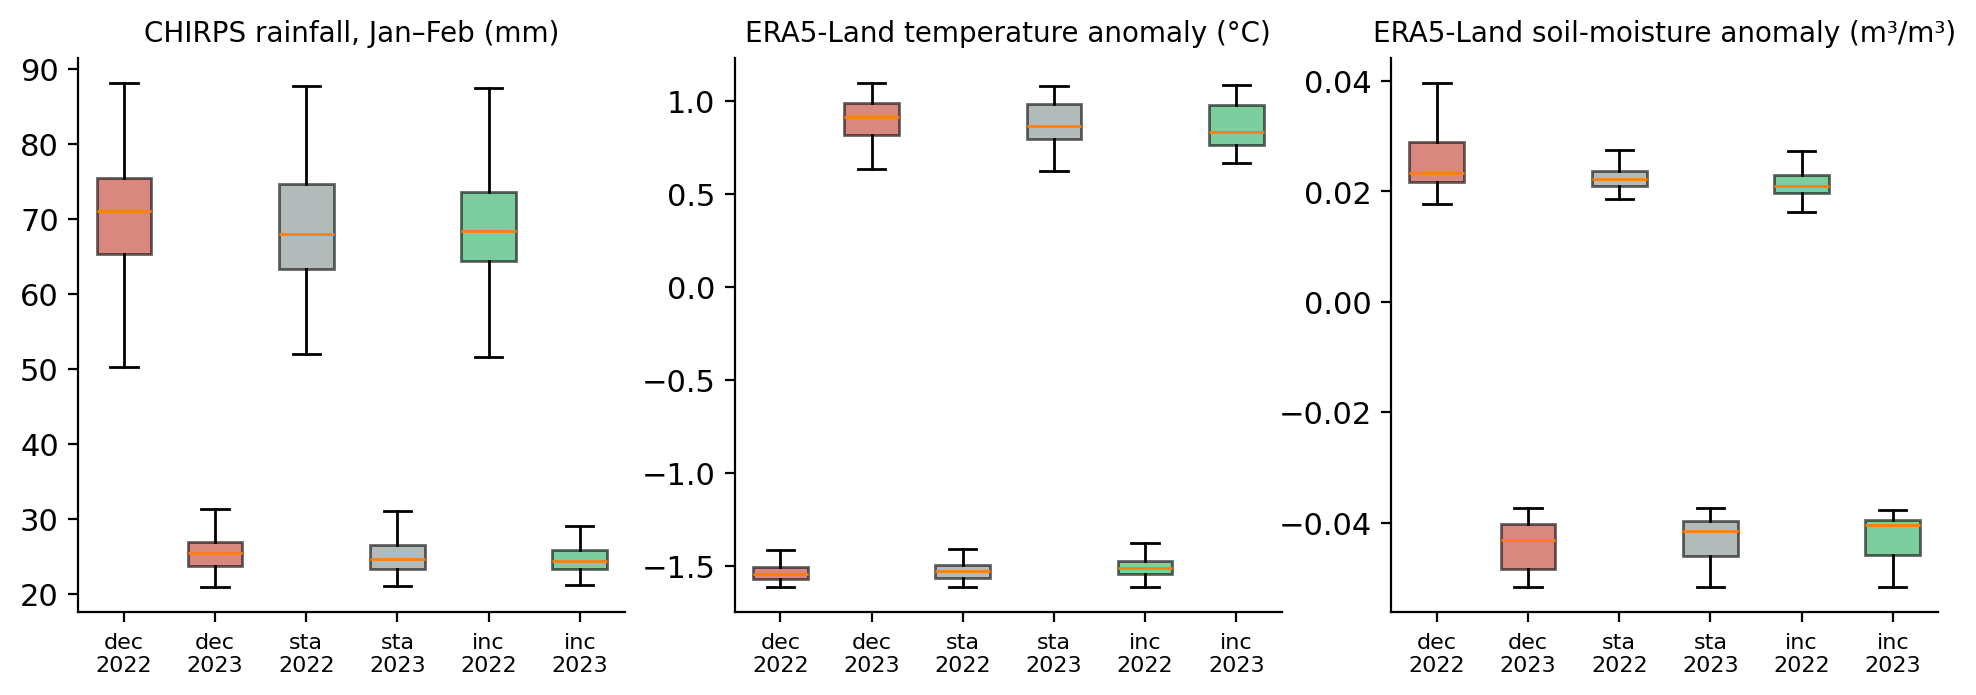
\includegraphics[width=\textwidth]{figures/fig_climate_by_class.png}
\caption{Rainfall, temperature anomaly and soil-moisture anomaly by class and year. The three classes are indistinguishable; only the year differs (\file{data/raw_metadata/selected_patches.csv}).}
\label{fig:climate}
\end{figure}

Climate values are attached to each patch by \texttt{reduce\_coarse}, which averages the coarse grid inside a square the size of one coarse pixel around the patch centre. The exported rainfall and ERA5 GeoTIFFs are therefore 1\,$\times$\,1 pixel.

\section{Source 5: terrain from NASADEM}

NASADEM is a reprocessed version of the elevation data from the Shuttle Radar Topography Mission (February 2000), at about 30\,m \citep{nasadem2020}. Earth Engine's \texttt{ee.Terrain.products} derives \textbf{slope} (steepness, degrees) and \textbf{aspect} (the direction a slope faces, degrees clockwise from north). Patch elevations range from 471 to 923\,m, mean slope is 6.4\dg, and only 19 patches have slopes of 12\dg{} or more.

\begin{whybox}
Terrain helps interpretation: steep slopes create shadows in optical images and distortions in radar images, and aspect affects moisture and therefore leaf fall. Terrain does not change within a year, so it is context, not evidence of change.
\end{whybox}

\section{The five sources at a glance}

\begin{table}[H]
\centering
\caption{The five data sources as used in the project. ``Export scale'' is the \texttt{scale} passed to Earth Engine (\file{src/gee_utils.py}).}
\label{tab:sources}
\small
\begin{tabularx}{\textwidth}{L{2.1cm}YYL{1.3cm}L{2.0cm}}
\toprule
Source & Earth Engine collection & Variables & Scale & Scenes / days \\
\midrule
Sentinel-2 L2A & \file{COPERNICUS/S2_SR_HARMONIZED} & 10 bands; NDVI, EVI, NDMI, NBR & 10\,m & 20 (T0), 23 (T1) \\
Sentinel-1 GRD & \file{COPERNICUS/S1_GRD} (IW, descending) & VV, VH (dB) & 10\,m & 15 (T0), 20 (T1) \\
CHIRPS & \file{UCSB-CHG/CHIRPS/DAILY} & rainfall total (mm) & 5,566\,m & 58 days each \\
ERA5-Land & \file{ECMWF/ERA5_LAND/MONTHLY_AGGR} & temperature and soil-moisture anomalies & 11,132\,m & Jan + Feb \\
NASADEM & \file{NASA/NASADEM_HGT/001} & elevation, slope, aspect & 30\,m & static \\
\bottomrule
\end{tabularx}
\end{table}

\begin{foryourreport}
\textbf{Study area} (about 400 words, with a map):
\begin{itemize}
  \item Location, districts, core/buffer/total area and forest types, citing \citet{kanha2026}.
  \item Why Kanha (handbook reasons) and why January--February.
  \item The rectangle's corners and area, and that it is larger than the reserve.
  \item A map: the whole of India (official boundary, not trimmed at the top), Madhya Pradesh, the reserve and the rectangle with patch points (your professor asks for this; see Chapter~\ref{ch:figures}).
\end{itemize}
\textbf{Data sources} (about 600 words):
\begin{itemize}
  \item Table~\ref{tab:sources} as a real table, with a citation for each source: \citet{drusch2012}, \citet{torres2012}, \citet{funk2015}, \citet{munozsabater2021}, \citet{nasadem2020}, and \citet{gorelick2017} for Earth Engine.
  \item Cloud masking, median composites, the harmonized collection, the descending orbit, only Sentinel-1A available.
  \item The four index equations (Equations~\ref{eq:ndvi}--\ref{eq:nbr}) with their citations, and the change definition (Equation~\ref{eq:delta}).
  \item The month-matched anomaly (Equation~\ref{eq:anomaly}).
\end{itemize}
\end{foryourreport}

\begin{selfcheck}
\begin{enumerate}
  \item Why does the project use the same two months in both years?
  \item Give the NDVI formula and say why a healthy canopy has a high NDVI.
  \item Why was the \emph{harmonized} Sentinel-2 collection needed for this project in particular?
  \item What is the difference between VV and VH, and which is more sensitive to vegetation?
  \item Radar backscatter fell by about 0.5\,dB everywhere. Why is this probably not forest loss?
  \item Why can rainfall not explain why one patch declined and its neighbour increased?
\end{enumerate}
\end{selfcheck}

\chapter{Stage 02: Earth Engine export and image processing}
\label{ch:stage02}

Stage~02 turns five global datasets into a neat package for each patch. It has two halves: \textbf{export} in Google Earth Engine \citep{gorelick2017} (notebook 01) and \textbf{digital image processing}, or DIP, on your computer (notebook 02).

\section{The candidate pool}

\file{data/raw_metadata/composite_stats.csv} holds \textbf{1,200 candidate patches}, each with Earth Engine statistics: index means for both years, radar means, climate values, terrain, masked fraction and the changes (for example \texttt{ndvi\_change}). The pool was made in an earlier (``parent'') repository and copied in. All candidate centres lie inside the study rectangle.

\begin{figure}[H]
\centering
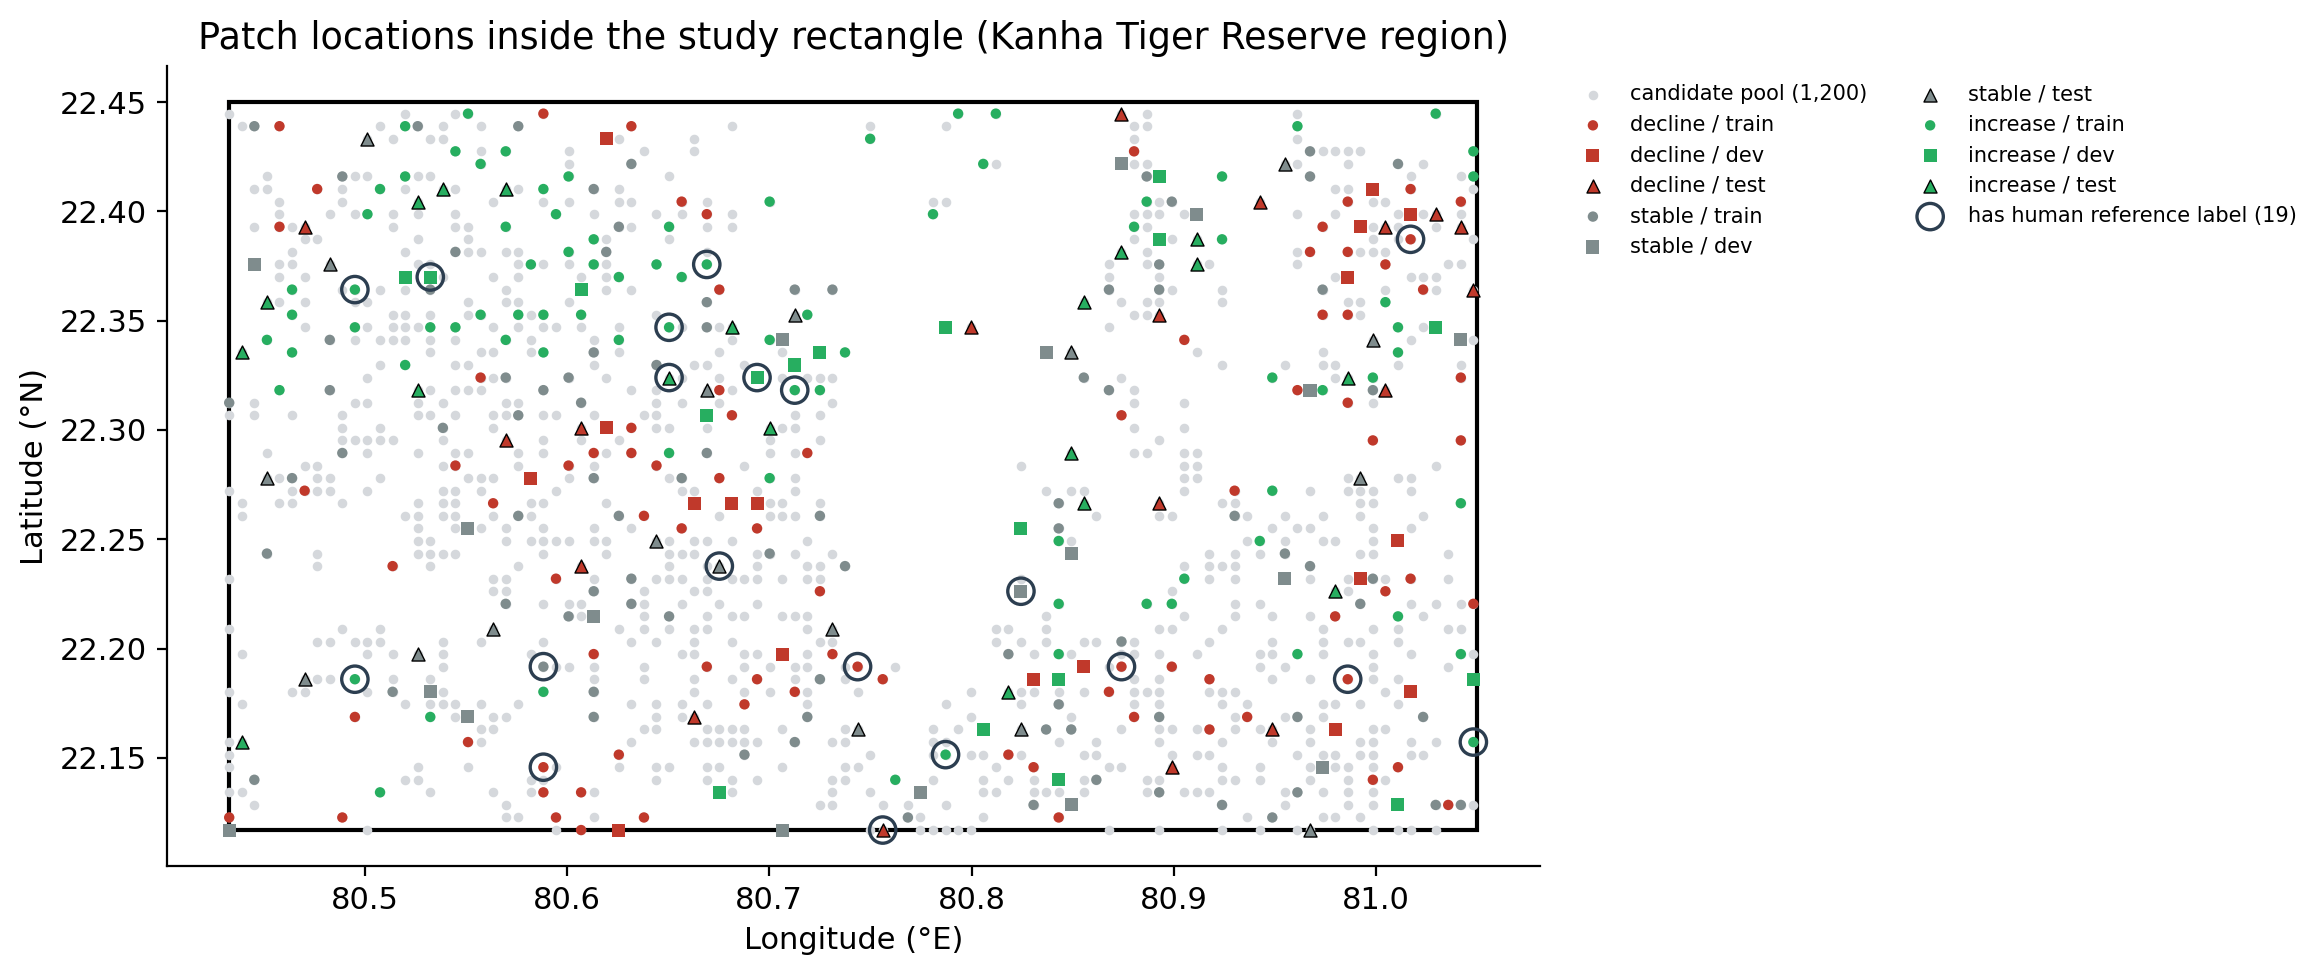
\includegraphics[width=\textwidth]{figures/fig_patch_map.png}
\caption{All 1,200 candidate centres (grey) and the 366 selected patches, coloured by class, with marker shape showing the split. Circles mark the 19 patches with a human label. Made by \file{study_guide/make_figures.py} from \file{data/raw_metadata/}.}
\label{fig:patchmap}
\end{figure}

\begin{watchout}
The pool has an empty vertical strip near 80.75--80.85\dg E (Figure~\ref{fig:patchmap}). The parent repository does not record why. The most likely reason is a forest-cover filter (for example, farmland or a valley without forest), but you do not know this. In the report, describe the strip and say the reason was not recorded; do not invent one.
\end{watchout}

\section{Patch geometry}

Each patch is built around its centre point (\texttt{patch\_geometry}): a circle of radius 320\,m is drawn (half of $64 \times 10$\,m), its bounding square is taken, and the square is intersected with the study rectangle. So a patch is a square of about 640\,m, and patches on the edge of the rectangle are cut short.

\begin{watchout}
The export did not set a projected coordinate system, so Earth Engine used EPSG:4326 (degrees). One pixel is 0.0000898\dg, which is 10.0\,m north--south but only about 9.3\,m east--west at 22\dg N, because lines of longitude converge. The planned 64\,$\times$\,64 patches therefore came out as about 70\,$\times$\,65 pixels (302 of 366 patches; another 50 are 69\,$\times$\,65), and edge patches are smaller (p00052 is 70\,$\times$\,30). Nothing breaks, but if you write ``64\,$\times$\,64 pixels'' add ``about 640\,m, exported in geographic coordinates''.
\end{watchout}

\section{The export}

\begin{wherecode}
Notebook \file{notebooks/01_gee_extraction.ipynb} (the version actually run) and \file{scripts/01_export_gee.py}; helpers in \file{src/gee_utils.py} and \file{src/export_utils.py}.
\end{wherecode}

\begin{enumerate}
  \item Earth Engine builds every composite \emph{once} for the whole rectangle: Sentinel-2 medians for T0 and T1, Sentinel-1 medians (descending), CHIRPS totals, ERA5-Land anomalies, NASADEM terrain, the true-colour images, and \dndvi{} and \dnbr.
  \item For each patch, every layer is clipped to the patch square and downloaded with \texttt{geemap.ee\_export\_image} straight into \file{data/raw_tiffs/}.
  \item Work runs in batches of 100 with a log (\file{data/raw_metadata/local_export_log.txt}) and a state file, so a crash can resume without downloading everything again.
\end{enumerate}

\begin{table}[H]
\centering
\caption{The 15 GeoTIFFs exported per patch (\texttt{PATCH\_SUFFIXES} in \file{src/export_utils.py}); 5,490 files for 366 patches.}
\label{tab:15files}
\small
\begin{tabular}{lll}
\toprule
File suffix & Content & Typical size (pixels) \\
\midrule
\texttt{\_T0\_rgb}, \texttt{\_T1\_rgb} & B4, B3, B2 as reflectance (0--1) & 70\,$\times$\,65 \\
\texttt{\_T0\_s2\_optical}, \texttt{\_T1\_s2\_optical} & the 10 Sentinel-2 bands & 70\,$\times$\,65 \\
\texttt{\_T0\_indices}, \texttt{\_T1\_indices} & NDVI, EVI, NDMI, NBR & 70\,$\times$\,65 \\
\texttt{\_T0\_s1}, \texttt{\_T1\_s1} & VV, VH (dB) & 70\,$\times$\,65 \\
\texttt{\_T0\_rainfall}, \texttt{\_T1\_rainfall} & CHIRPS total (mm) & 1\,$\times$\,1 \\
\texttt{\_T0\_era5}, \texttt{\_T1\_era5} & temperature and soil-moisture anomalies & 1\,$\times$\,1 \\
\texttt{\_dem} & elevation, slope, aspect & about 24\,$\times$\,22 \\
\texttt{\_delta\_ndvi}, \texttt{\_delta\_nbr} & T1 $-$ T0 change & 70\,$\times$\,65 \\
\bottomrule
\end{tabular}
\end{table}

\begin{whybox}
Local download with \texttt{geemap} is faster than Earth Engine's ``export to Google Drive'' for small images; the Drive route stays as a fallback (\texttt{mode: drive} in the config, \file{scripts/02_download_drive.py}). Keeping all 15 layers, not only the colour images, means later experiments need no new download.
\end{whybox}

\subsection{Missing data}

Candidates whose masked fraction was above 0.15 (15\,\%) in either year were labelled ``uncertain'' and never sampled. For the 366 selected patches the masked fraction is between 0.8\,\% and 2.3\,\% (\file{data/raw_metadata/selected_patches.csv}).

\begin{watchout}
\texttt{masked\_frac\_before} and \texttt{masked\_frac\_after} are identical for all 366 patches. Real cloud masks for two different years would differ, so this value probably measures pixels lost at patch edges, not cloud. Describe it as ``very little missing data'', not as a measured cloud fraction.
\end{watchout}

\section{Image processing (DIP)}

Notebook \file{02_dip_auto_classify.ipynb} (``DIP + five-source packaging'') prepares what the models will see.

\subsection{Making the colour images look right}

Reflectance values of forest are small (about 0.02--0.1 in visible light), so they must be \emph{stretched} to the 0--255 display range. The first version stretched each band separately using percentiles. On small, dark forest chips this exaggerated noise and shifted the colours, producing purple images (Figure~\ref{fig:purple}). The fix was a fixed window: divide every band by 0.22 and clip to $[0, 1]$ (\texttt{percentile\_stretch\_rgb} in \file{src/dip_utils.py}, \texttt{vmax=0.22}), the same as the common Earth Engine display setting \texttt{min: 0, max: 2200}. It keeps the relative colours of the three bands, so forest looks green-brown.

\begin{figure}[H]
\centering
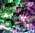
\includegraphics[width=0.22\textwidth]{figures/fig_purple.jpg}\hspace{1cm}
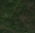
\includegraphics[width=0.22\textwidth]{figures/fig_natural.jpg}
\caption{The same chip with the first per-band stretch (left, purple) and with the fixed reflectance window used in the final pipeline (right). From \file{slides/figures/}.}
\label{fig:purple}
\end{figure}

\subsection{Padding and resizing to a 512\,$\times$\,512 canvas}

Vision--language models expect square images, and one canvas size lets every layer share the same coordinates (\texttt{pad\_and\_resize}):
\begin{enumerate}
  \item \textbf{Pad to a square} with zeros, split between both sides. A 65\,$\times$\,70 chip gets 5 rows of black.
  \item \textbf{Resize} the square to 512\,$\times$\,512: bilinear interpolation for colour images (smooth), nearest-neighbour for single-band arrays (keeps the original values).
  \item \textbf{Move any boxes} with the image: $x' = (x + p_x)\,s$, $y' = (y + p_y)\,s$, with $s = 512/\max(H, W)$ and $p_x, p_y$ the left and top padding.
\end{enumerate}

\begin{watchout}
Two consequences come back later.
\begin{enumerate}
  \item \textbf{No new detail.} Enlarging a 70-pixel chip to 512 pixels (about 7.3 times) only makes each pixel a bigger block. On the laptop the images were then shrunk again (longer side at most 336 pixels).
  \item \textbf{Padding enters the averages.} The arrays of indices and radar values are padded with 0, and the evidence card later averages the whole 512\,$\times$\,512 canvas, zeros included. For a 65-row chip padded to 70 rows, every mean is multiplied by about $65/70 = 0.93$; for the edge patch p00052 (30 rows) by about $30/70 = 0.43$. Chapter~\ref{ch:stage03} shows the effect on the card (the ``padding bias'').
\end{enumerate}
\end{watchout}

\subsection{Otsu thresholding: finding the pixels that dropped most}

\begin{plainwords}
Otsu's method tries every possible threshold and picks the one that splits the pixels into two groups that are as different from each other as possible, each group being as uniform as possible inside.
\end{plainwords}

If $p_i$ is the share of pixels in histogram bin $i$, a threshold $t$ splits them into two groups with weights $\omega_0(t)$, $\omega_1(t)$ and means $\mu_0(t)$, $\mu_1(t)$. Otsu picks the $t$ that maximises the between-group variance \citep{otsu1979}:
\begin{equation}
\sigma_B^2(t) = \omega_0(t)\,\omega_1(t)\,\bigl[\mu_0(t)-\mu_1(t)\bigr]^2 .
\label{eq:otsu}
\end{equation}

The project applies it to change maps (\texttt{process\_tensor\_otsu} in \file{src/dip_utils.py}):
\begin{enumerate}
  \item read the \dndvi{} (or \dnbr) raster and keep only \emph{drops} larger than \texttt{min\_drop} (0.04 in notebook 02);
  \item if fewer than 16 pixels dropped, return an empty mask; otherwise run Otsu on the drop sizes and keep the pixels above the threshold;
  \item clean the mask with \textbf{morphological closing} (a 3\,$\times$\,3 dilation followed by an erosion), which fills small holes;
  \item trace each separate blob, enclose it in the smallest upright \textbf{bounding box}, and drop boxes smaller than 64 pixels.
\end{enumerate}

If an NBR-drop box overlaps an NDVI-drop box with \textbf{intersection over union}
\begin{equation}
\mathrm{IoU}(A,B) = \frac{|A\cap B|}{|A\cup B|} \ge 0.4,
\label{eq:iou}
\end{equation}
the two are merged and called \emph{Fire} (a burn lowers both indices); other NDVI boxes are called \emph{Deforestation}. Each box gets a severity from its mean drop (Deforestation: low below 0.08, high from 0.25; Fire: low below 0.10, high from 0.27, matching the lower bounds of two burn-severity classes in \citet{keybenson2006}). Each box is stored as a \textbf{triplet} \texttt{[[x\_min, y\_min, x\_max, y\_max], type, severity]}.

\begin{watchout}
Otsu run on the drops alone always splits them into ``smaller'' and ``larger'' drops, even in a patch where all drops are tiny noise. The mask is relative to each patch, not proof that disturbance happened.
\end{watchout}

\subsection{Why only three patches have boxes}

After the boxes are made, \texttt{apply\_reference\_class\_policy} (\file{src/dip_utils.py}) removes all boxes when the patch's \emph{human} label is \texttt{stable}, \texttt{increase}, \texttt{uncertain} \textbf{or empty}. Because 347 of the 366 patches have no human label, almost every box disappeared. Only three patches keep boxes (p00052, p01289, p01371; six boxes, all ``Deforestation, Low''), all labelled \texttt{decline} by both the rule and the person.

\begin{figure}[H]
\centering
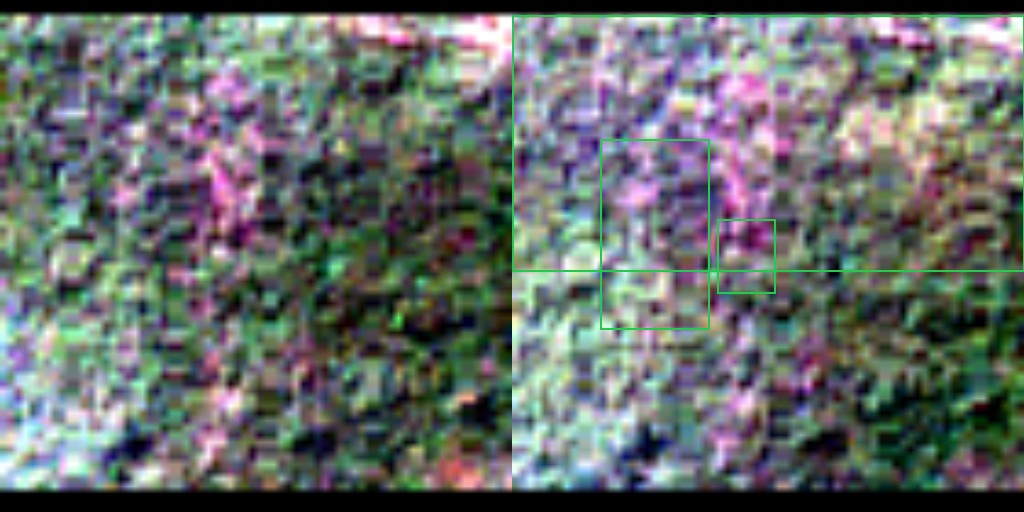
\includegraphics[width=0.72\textwidth]{figures/fig_otsu_p01289.jpg}
\caption{Otsu boxes for p01289 on the T0 (left) and T1 (right) chips, from \file{data/qa_figures/_spotcheck/}. This spot-check was made before the colour fix, so it still shows the purple stretch.}
\label{fig:otsu}
\end{figure}

\begin{watchout}
The September slides describe ``explanations tied to bounding boxes'', but in the final dataset the boxes play almost no role, and the models were never asked about them. The intended rule was probably ``remove boxes when the person says stable or increase''; treating an empty label the same way was a side effect. In the report, mention the boxes briefly as an implemented step that ended up covering three patches, or leave them out.
\end{watchout}

\subsection{What is saved}

\begin{itemize}
  \item Colour canvases as JPEG, quality 95: \file{data/processed_images/pXXXXX_T0.jpg} and \file{_T1.jpg}.
  \item Physical layers as NumPy arrays (\texttt{.npy}), 13 per patch (optical bands, indices, radar, rainfall and ERA5 for both years, terrain, \dndvi, \dnbr), and the Otsu masks in \file{data/evidence_masks/}.
  \item A record of all triplets in \file{data/raw_metadata/triplets.json}.
\end{itemize}

\begin{foryourreport}
In ``Preprocessing and Patch Generation'' (about 450 words):
\begin{itemize}
  \item The candidate pool (1,200), the patch geometry (320\,m circle $\rightarrow$ square $\rightarrow$ clipped to the rectangle), and the export in degrees (about 70\,$\times$\,65 pixels).
  \item The 15 layers per patch (Table~\ref{tab:15files} can go in an appendix).
  \item The masked-fraction filter (0.15) and the very low missing data.
  \item Padding to a square and resizing to 512\,$\times$\,512, saying that this enlarges the chips about seven times and adds no detail.
  \item Otsu, boxes and the policy in two or three sentences at most, since only three patches kept boxes. Equation~\ref{eq:otsu} is optional.
\end{itemize}
Avoid ``the images were downsampled to 512\,$\times$\,512'': they were padded and \emph{enlarged}.
\end{foryourreport}

\begin{selfcheck}
\begin{enumerate}
  \item Why did the ``64\,$\times$\,64'' patches come out as about 70\,$\times$\,65 pixels?
  \item Why is the masked fraction probably not a cloud measurement?
  \item What does padding with zeros do to the averages written into the evidence card?
  \item In one sentence, what does Otsu's method choose?
  \item Why do only three patches have bounding boxes?
\end{enumerate}
\end{selfcheck}

\chapter{Stage 03: labels and evidence cards}
\label{ch:stage03}

Stage~03 produces three things for every patch (the three orange boxes in your workflow figure): the pair of colour images (Chapter~\ref{ch:stage02}), the \textbf{automatic label}, and the \textbf{evidence card}. This chapter explains the last two, because every result in the report depends on them.

\section{The automatic label}
\label{sec:labels}

\subsection{The rule}

Notebook 01, cell 17, assigns \texttt{candidate\_class} from each patch's mean NDVI change $\Delta$ and the 15th and 85th percentiles of $\Delta$ over the 1,200-patch pool, $q_{15} = -0.0377$ and $q_{85} = +0.0031$:
\begin{equation}
\text{class} =
\begin{cases}
\text{uncertain} & \text{masked fraction} > 0.15 \text{ in either year,}\\
\text{decline} & \Delta \le q_{15},\\
\text{increase} & \Delta \ge q_{85},\\
\text{stable} & |\Delta| < 0.05,\\
\text{uncertain} & \text{otherwise.}
\end{cases}
\label{eq:labelrule}
\end{equation}
Uncertain patches were never sampled. Because both percentiles lie inside $\pm0.05$, every unmasked patch between $q_{15}$ and $q_{85}$ is labelled stable, and the last ``uncertain'' case never happens for this pool. In practice the rule is: \emph{bottom 15\,\% of NDVI change is decline, top 15\,\% is increase, the rest is stable}.

\begin{whybox}
The roadmap (Section~6) says to ``begin with region-specific quantiles rather than claiming universal ecological thresholds''. Percentiles guarantee enough examples of each class even in a year with little real change, and they avoid borrowing thresholds from studies of other forests.
\end{whybox}

\begin{figure}[H]
\centering
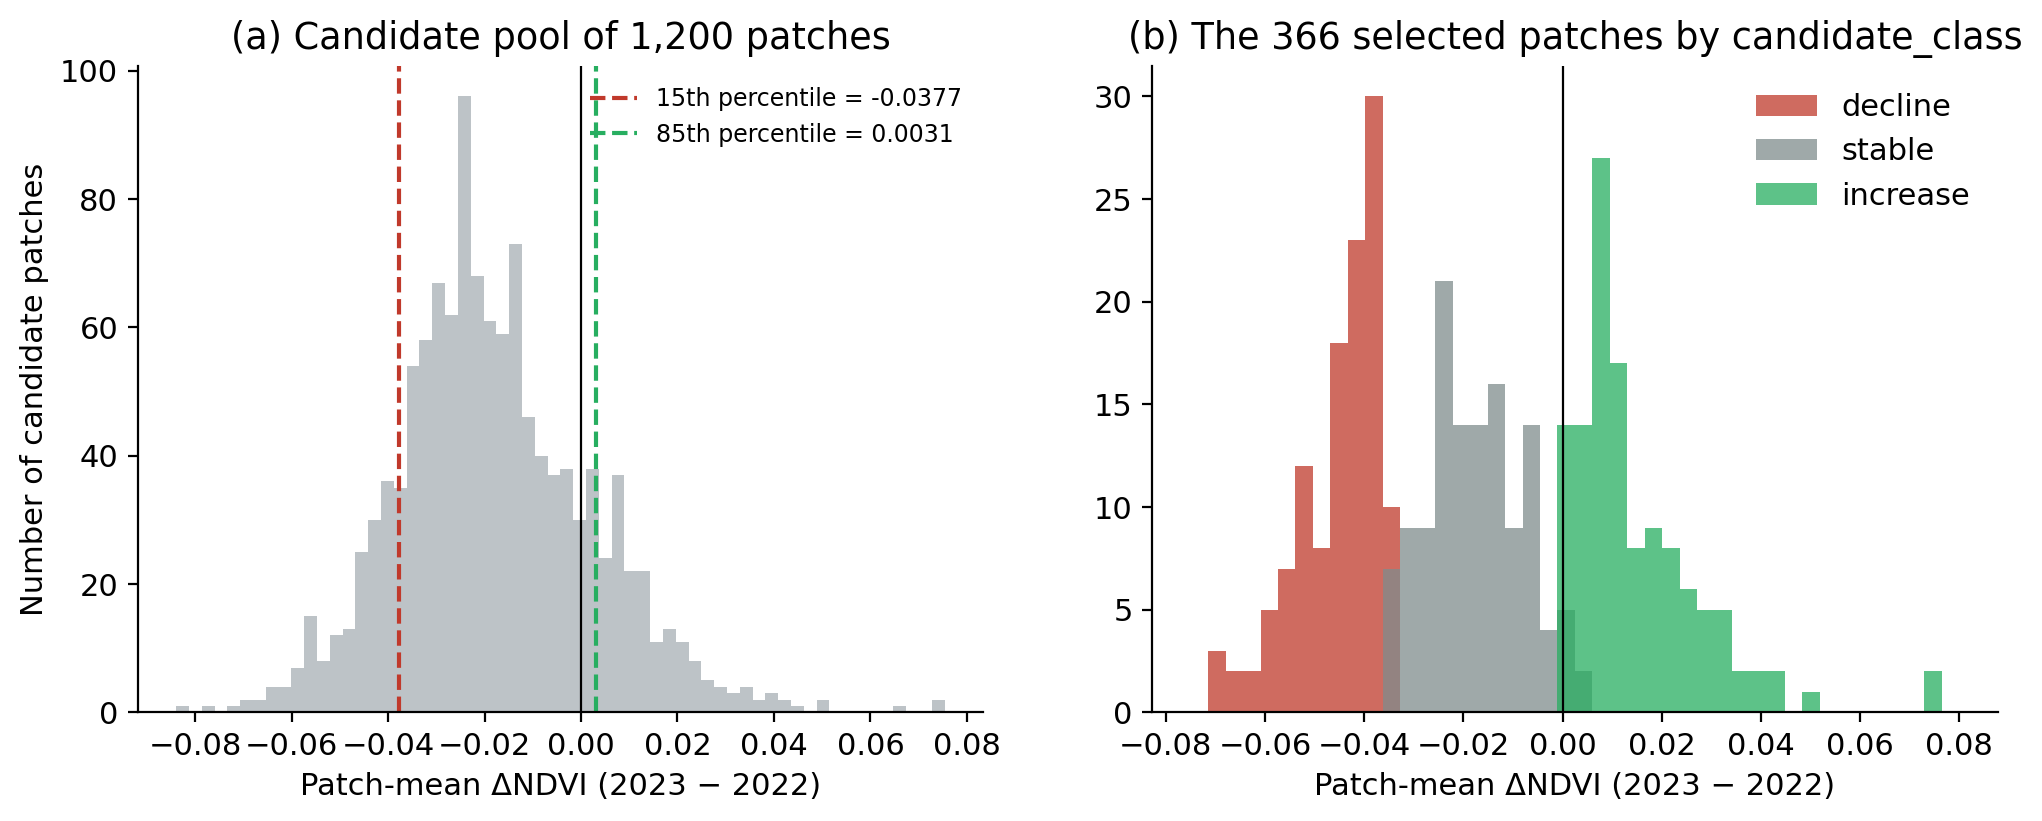
\includegraphics[width=\textwidth]{figures/fig_ndvi_labels.png}
\caption{(a) Patch-mean \dndvi{} over the 1,200-patch pool with the 15th and 85th percentiles; most patches lost a little greenness. (b) \dndvi{} of the 366 selected patches by label. From \file{data/raw_metadata/}.}
\label{fig:ndvilabels}
\end{figure}

\subsection{How the 366 patches were chosen}

The first 300 patches (100 per class) were selected in the parent repository. Notebook 01, cell 17, then added up to 25 per class from the rest of the pool, keeping new centres at least 960\,m (1.5 patch widths) from all existing ones; only 22 decline candidates passed that distance filter. This gave 372 patches. Six had incomplete exports and were moved to \file{data/outcasts/}, leaving \textbf{366: 120 decline, 124 stable, 122 increase}.

\begin{watchout}
For the 72 added patches the percentiles were recomputed on the \emph{remaining} pool, so their cut-offs differ slightly from those of the first 300. The class ranges therefore overlap a little: decline patches reach $\Delta = -0.034$ while stable patches go down to $-0.036$, and increase patches go down to $-0.001$ while stable patches reach $+0.003$ (Figure~\ref{fig:ndvilabels}b). The labels are almost, but not exactly, a function of $\Delta$.
\end{watchout}

\subsection{What the labels really mean}

\begin{plainwords}
The whole region became slightly less green between the two years (mean \dndvi{} $= -0.016$, standard deviation 0.027). So the percentile rule calls ``increase'' anything in the greenest 15\,\%, even if it barely changed: an increase patch has \dndvi{} anywhere from $-0.001$ to $+0.075$, and half of them changed by less than 0.011. ``Decline'' means ``among the 15\,\% that lost the most greenness'', here a drop of about 0.034 to 0.071. ``Stable'' means ``in between''. Only 34 of the 366 patches changed NDVI by 0.05 or more in either direction.
\end{plainwords}

The labels are \textbf{relative ranks within this region and pair of years}, not absolute ecological states. That is acceptable for a benchmark if you say it clearly. It is wrong to call increase patches ``recovering forest'' or decline patches ``degraded'' or ``deforested''.

\section{The human check}
\label{sec:humanlabels}

The roadmap asked for manual validation and an independent audit. What was done:

\begin{itemize}
  \item \textbf{Pilot, early September}: 36 patches reviewed by a person; automatic and human labels agreed on 17 of 36 (47\,\%) (\file{summary.txt}).
  \item \textbf{Final dataset}: 19 patches carry a \texttt{reference\_class} (13 train, 3 development, 3 test). The automatic label agrees on \textbf{8 of 19 (42\,\%; 95\,\% interval 23--64\,\%)} (\file{results/preflight_report.json}). The other pilot patches are kept in \file{data/pilot_reference/}.
  \item No second reviewer and no expert audit.
\end{itemize}

\begin{table}[H]
\centering
\caption{Automatic label against human label for the 19 patches in the final dataset (rows: automatic; columns: human).}
\label{tab:humanagree}
\begin{tabular}{lccc|c}
\toprule
 & human decline & human stable & human increase & total \\
\midrule
auto decline & 3 & 2 & 1 & 6 \\
auto stable & 0 & 2 & 1 & 3 \\
auto increase & 4 & 3 & 3 & 10 \\
\midrule
total & 7 & 7 & 5 & 19 \\
\bottomrule
\end{tabular}
\end{table}

Some disagreements are large: p01350 lost 0.040 NDVI but the person called it ``increase''; p03545 and p04416 gained NDVI but were called ``decline''. The person presumably judged the colour images, where changes this small are hard to see, while the rule reads a number the eye cannot see. Neither is ``truth''. Only 3 of the 10 automatic \texttt{increase} patches that were checked were confirmed, so \texttt{increase} is the least reliable class.

\begin{foryourreport}
The repository does not record how the human labels were made. Write down your actual procedure (who looked, at what images, with which instructions) and report it in Methods. Report the agreement as ``8 of 19 (42\,\%)'' with the interval, and call the automatic labels ``operational reference labels'' or ``automatic labels'', not ``ground truth''.
\end{foryourreport}

\section{The evidence card}
\label{sec:card}

\subsection{Two versions of the text}

\begin{enumerate}
  \item \textbf{Version 1} (\file{scripts/03_build_dataset.py}) tried to have a local language model (through Ollama) write an explanation for each patch. Ollama was not running, so all 366 fell back to a fixed template filled with numbers (\file{results/preflight_report.json}: ``ollama=0, fallback=366''). These texts survive only in \file{dataset_old.jsonl}.
  \item \textbf{Version 2} (\file{scripts/build_extensive_jsonl.py}, \texttt{enrich\_row} in \file{src/extensive_descriptions.py}) replaced them with text \emph{computed from the rasters}. Every record in the final \file{dataset.jsonl} has \texttt{explanation\_source = raster\_analysis\_v2}, and all 366 texts are different.
\end{enumerate}

\begin{newinfo}
Your current draft says that ``all narrative explanations are just templates, because no language model based explanation was obtained''. That sentence came from the rewrite I gave you earlier, and it is wrong for the final dataset: the stored text is a rule-based narrative computed from each patch's rasters. What is true is that \emph{no language model wrote it}. Correct the sentence (Chapter~\ref{ch:draft}).
\end{newinfo}

\subsection{How version 2 is built}

For each patch, \texttt{enrich\_row}:
\begin{enumerate}
  \item reads the colour GeoTIFFs and measures brightness and ``green cover'' (the share of pixels where green is the largest channel);
  \item loads the 512\,$\times$\,512 arrays of indices, radar and \dndvi{} and computes means, percentiles and the share of pixels that fell below $-0.05$ or rose above $+0.05$;
  \item takes rainfall, ERA5-Land and terrain values from the record;
  \item turns numbers into words with simple rules (Table~\ref{tab:inferrules});
  \item assembles a narrative and the model prompt, \texttt{condition\_c\_user\_prompt}.
\end{enumerate}

\begin{table}[H]
\centering
\caption{Rules that convert measurements into the words on the card (\texttt{\_infer\_signals} in \file{src/extensive_descriptions.py}).}
\label{tab:inferrules}
\small
\begin{tabularx}{\textwidth}{lY}
\toprule
Field & Rule \\
\midrule
vegetation\_trend & strong\_decline if \dndvi{} $\le -0.04$ and at least 8\,\% of pixels dropped by more than 0.05; moderate\_decline if \dndvi{} $\le -0.02$; greening if $\ge +0.02$ and at least 8\,\% rose by more than 0.05; slight\_greening if $\ge +0.01$; otherwise stable \\
fire\_burn\_likelihood & elevated\_burn\_signal if the NBR mask exceeds the NDVI mask by 2 points and \dnbr{} $< -0.02$; deforestation\_pattern if the NDVI mask exceeds 2\,\% and boxes exist; otherwise low \\
candidate\_class\_consistency & agrees if the label and the trend point the same way; spatial\_anomaly if the label is stable but boxes exist; otherwise partial\_mismatch \\
sar\_evidence\_strength & notable\_backscatter\_shift if $|\Delta\mathrm{VV}| \ge 0.8$\,dB, otherwise secondary \\
climate\_evidence\_strength & drier\_second\_window if rainfall fell by at least 25\,mm; wetter if it rose by at least 25\,mm; otherwise neutral \\
terrain\_context & steep\_terrain if slope $\ge 12^\circ$, otherwise gentle\_terrain \\
\bottomrule
\end{tabularx}
\end{table}

\subsection{A real card, with the line that matters}

This is the text that Qwen2-VL-2B and LLaVA received in Track~A for test patch p00575 (gold label \texttt{decline}):

\begin{tcolorbox}[colback=gray!4,colframe=gray!50,fontupper=\scriptsize\ttfamily,breakable]
Task: ground\_forest\_disturbance\_in\_spectral\_evidence\\
Condition C evidence (measured on disk, analysis v2):\\
T0 (2022) terrain RGB (65$\times$69 native, stretched for display): brightness=0.169, green-cover=0.74, uniform illumination; canopy-green dominates. T1 (2023) terrain RGB (65$\times$69 native, stretched for display): brightness=0.198, green-cover=0.42, uniform illumination; mixed canopy and non-photosynthetic pixels. Brightness change T1$-$T0=+0.0292 on natural-color chips.\\
On the 512$\times$512 aligned stack, mean NDVI 0.6248$\rightarrow$0.5752 ($\Delta$=-0.0496), NBR 0.3106$\rightarrow$0.3135 ($\Delta$=+0.0029), EVI $\Delta$=-0.0040, NDMI $\Delta$=-0.0070. $\Delta$NDVI raster: mean=-0.04966, 48.9\% pixels below $-$0.05, 0.4\% above +0.05; $\Delta$NBR raster mean=0.0029.\\
SAR (512$\times$512 means): VV -8.624$\rightarrow$-8.839 dB ($\Delta$-0.22), VH -14.322$\rightarrow$-14.734 dB ($\Delta$-0.41); interpreted as secondary.\\
CHIRPS Jan--Feb total 72.5$\rightarrow$25.4 mm ($\Delta$-47.1 mm, drier\_second\_window). ERA5-Land anomalies: temperature -1.50$\rightarrow$+1.08 \textdegree C, soil moisture +0.027$\rightarrow$-0.048 vs 2015--2021 climatology.\\
NASADEM at patch center: 834 m, slope 5.1\textdegree, aspect 160\textdegree{} (gentle\_terrain).\\
No Otsu boxes (NDVI mask active on 21.7\% of pixels, NBR mask on 3.5\%).\\
\colorbox{red!20}{Inference for p00575: vegetation\_trend=strong\_decline,}\\
\colorbox{red!20}{burn/deforestation cue=low, candidate\_class=decline}\\
\colorbox{red!20}{(agrees with spectra/boxes).}\\
Respond with class (stable/decline/increase) and a short grounded explanation.
\end{tcolorbox}

The highlighted line is the \textbf{pipeline's summary line}. \texttt{synthesize\_narrative} in \file{src/extensive_descriptions.py} builds every card from seven pieces, and the last piece, \texttt{conclusion}, is this summary. It was written for a human reader of the card, and it states \texttt{candidate\_class}, the same field that is used as the gold label. Because it is part of \texttt{condition\_c\_user\_prompt}, every full card given to a model contains the answer.

\begin{plainwords}
This is not a scandal; it is a fact about the input that must be stated. A model shown the full card can get a patch right by reading the label, by reading the numbers, by looking at the images, or by a mixture. Track~A's numbers therefore measure ``how well a model uses the complete card''. Chapter~\ref{ch:trackA} explains what the project did to separate these, and what it could not separate.
\end{plainwords}

\section{The card does not always agree with the label}

The card's \texttt{vegetation\_trend} words use a different rule from the label (Table~\ref{tab:inferrules}). Comparing the two over all 366 patches (Figure~\ref{fig:labeltrend}):
\begin{itemize}
  \item 258 patches agree and \textbf{108 disagree} (``partial\_mismatch'').
  \item Every \texttt{decline} patch has a declining trend (54 strong, 66 moderate).
  \item \textbf{61 of 122 \texttt{increase} patches} have the trend ``stable''.
  \item 47 of 124 \texttt{stable} patches have the trend ``moderate\_decline''.
\end{itemize}

\begin{figure}[H]
\centering
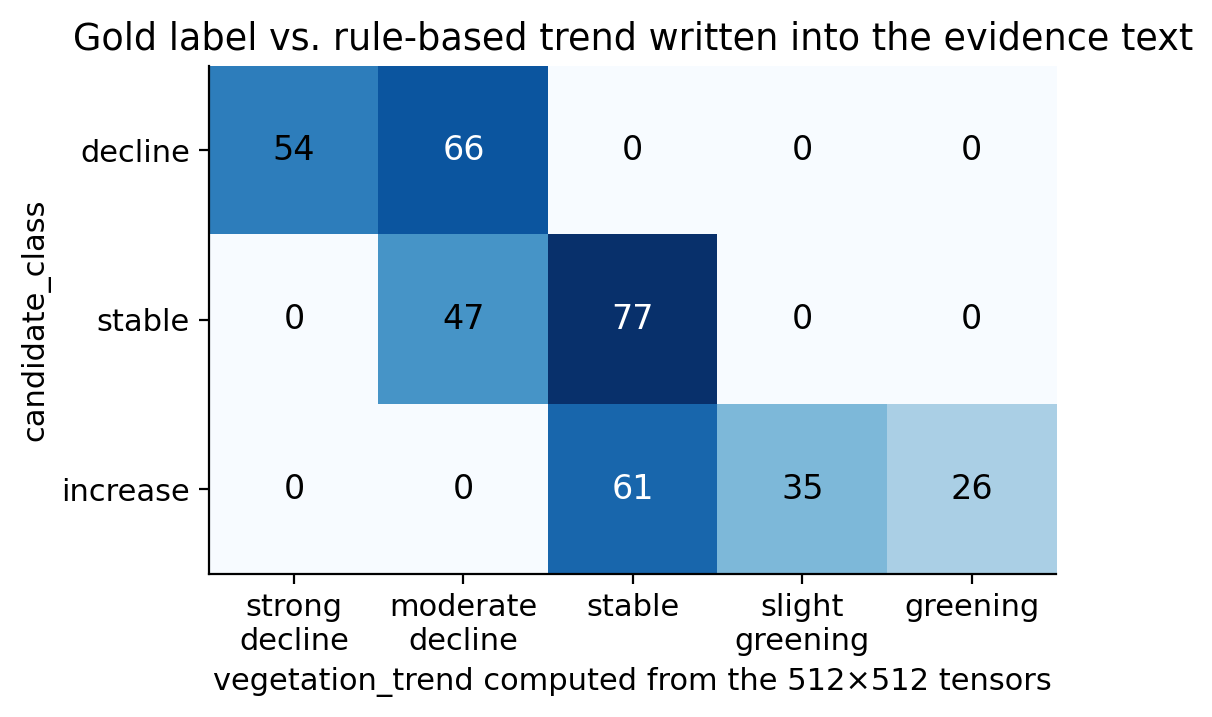
\includegraphics[width=0.78\textwidth]{figures/fig_label_vs_trend.png}
\caption{Gold label against the rule-based trend written into the evidence card (\file{dataset.jsonl}).}
\label{fig:labeltrend}
\end{figure}

The two disagree because they apply different thresholds to different numbers: the label uses the region's percentiles ($-0.038$ and $+0.003$) of the Earth Engine patch mean; the trend uses fixed cut-offs ($\pm0.02$ and $+0.01$) on the padded canvas mean. A model shown the full card can therefore receive two signals that point different ways: the trend word says ``stable'' while the summary line says \texttt{candidate\_class=increase}.

\section{The padding bias in the card's numbers}
\label{sec:padbias}

The means on the card are taken over the whole 512\,$\times$\,512 canvas, padding included (Chapter~\ref{ch:stage02}). If a fraction $f$ of the canvas is zero padding,
\begin{equation}
\bar{x}_{\text{reported}} = (1-f)\,\bar{x}_{\text{true}} + f\cdot 0 = (1-f)\,\bar{x}_{\text{true}} .
\end{equation}
For a normal 65-row chip, $1-f \approx 0.93$, so the NDVI on the card is about 7--8\,\% too low; averaged over all patches, the card's NDVI is 0.92 times the Earth Engine mean. For the clipped edge patch p00052 the factor is about 0.43, and its NDVI appears as 0.31 instead of about 0.7. Radar values (negative decibels) are pulled towards 0\,dB.

\begin{figure}[H]
\centering
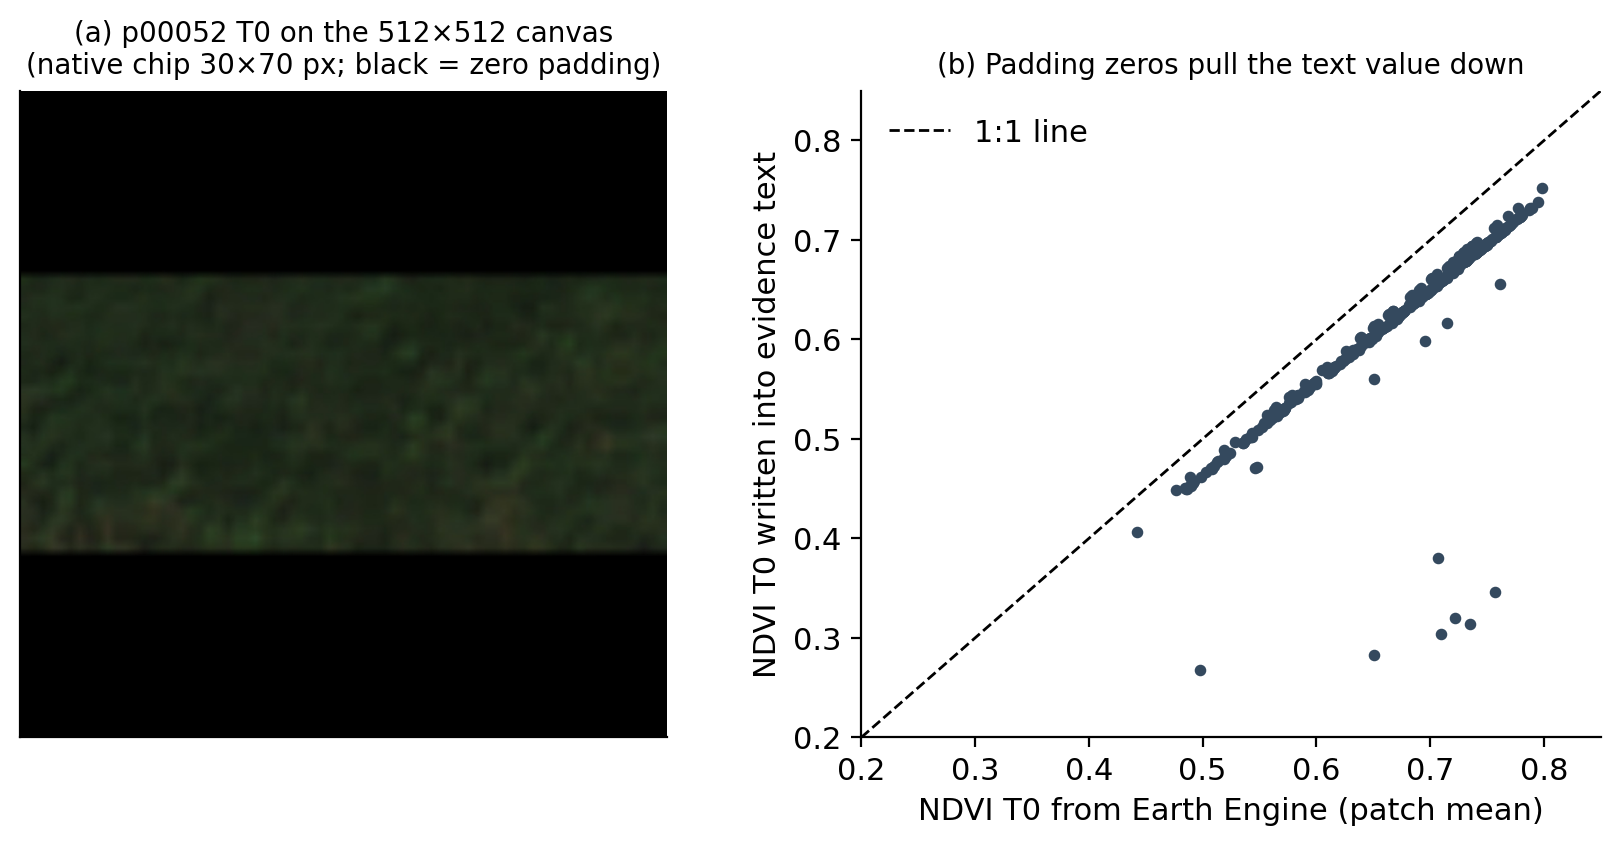
\includegraphics[width=0.9\textwidth]{figures/fig_padding_bias.png}
\caption{(a) An edge patch on the canvas: most of the image is padding. (b) NDVI written on the card against the Earth Engine patch mean; points below the 1:1 line are biased low, and the isolated low points are clipped edge patches.}
\label{fig:padbias}
\end{figure}

The \emph{changes} are scaled by the same factor, so their sign is right and they correlate 0.995 with the Earth Engine values, but their size is understated. The fix is simple for future work: pad the arrays with ``not a number'' instead of 0, or compute statistics on the original chip.

\begin{foryourreport}
In ``Change Evidence and Labelling'' (about 600 words):
\begin{itemize}
  \item The label rule as an equation (Equation~\ref{eq:labelrule}) and the two percentile values; say that the last case never occurs.
  \item The sampling (300 + 72, 960\,m spacing, 6 incomplete, final 120/124/122) and the slight class overlap.
  \item What the classes mean: relative ranks, small changes, 34 patches with $|\Delta| \ge 0.05$.
  \item The human check (8 of 19) and your procedure.
  \item The card: what it lists, that it was computed from the rasters (version 2), that its last line repeats \texttt{candidate\_class}, and that its trend words disagree with the label on 108 patches.
  \item The padding bias in one or two sentences (here or in Limitations).
\end{itemize}
\end{foryourreport}

\begin{selfcheck}
\begin{enumerate}
  \item State the labelling rule in one sentence without the equation.
  \item Why can a patch whose NDVI fell slightly be labelled \texttt{increase}?
  \item What are the two versions of the card text, and which one is in the final dataset?
  \item What is the summary line, and why does it matter for Track~A?
  \item Why do the card's trend words disagree with the label for 108 patches?
  \item Why is the NDVI written on the card about 8\,\% too low?
\end{enumerate}
\end{selfcheck}

\chapter{Stage 04: the frozen dataset and the split}
\label{ch:stage04}

Stage~04 is short in your workflow figure, but it fixes the rules of every experiment that follows: which file is the dataset, which patches may be used for training, and which patches are kept for the final test.

\section{The dataset file}

\file{dataset.jsonl} has one JSON record per line, 366 lines (3.9\,MB). ``JSON Lines'' is used because each record can be read on its own, which suits sending examples to a model one at a time.

\begin{longtable}{L{3.8cm}L{10.4cm}}
\caption{Fields of each record in \file{dataset.jsonl}.}\label{tab:jsonl}\\
\toprule
\textbf{Field} & \textbf{Content} \\
\midrule
\endfirsthead
\toprule
\textbf{Field} & \textbf{Content} \\
\midrule
\endhead
\texttt{id} & patch identifier, e.g.\ \texttt{p00575} \\
\texttt{task} & \texttt{ground\_forest\_disturbance\_in\_spectral\_evidence} \\
\texttt{images} & paths to the T0 and T1 JPEGs (512\,$\times$\,512) \\
\texttt{sentinel2}, \texttt{sentinel1} & band and index names, array and GeoTIFF paths, orbit pass, scene counts \\
\texttt{chirps}, \texttt{era5\_land}, \texttt{dem} & rainfall totals, climate anomalies, terrain values and paths \\
\texttt{evidence} & \dndvi{} and \dnbr{} arrays and Otsu masks \\
\texttt{acquisition} & season, windows, masked fractions \\
\texttt{triplets} & boxes with type and severity (empty for 363 patches) \\
\texttt{file\_analysis} & every computed statistic and the rule-based words of Table~\ref{tab:inferrules} \\
\texttt{text} & visual descriptions, spectral narrative, analyst description, the model prompt (\texttt{condition\_c\_user\_prompt}) and the summary line \\
\texttt{explanation}, \texttt{explanation\_source} & the rule-based narrative; \texttt{raster\_analysis\_v2} for all 366 \\
\texttt{candidate\_class} & the automatic label: the gold label for all scoring \\
\texttt{reference\_class} & the human label, or null (19 patches have one) \\
\texttt{sources\_present} & which of the five sources exist (all true) \\
\bottomrule
\end{longtable}

Latitude and longitude are deliberately removed from every record (\texttt{\_clean} in \file{scripts/03_build_dataset.py}), so a model cannot use location knowledge.

\section{Freezing and splitting}

\file{scripts/05_freeze_jsonl_and_splits.py} (24 September):
\begin{enumerate}
  \item copies the old \file{dataset.jsonl} to \file{dataset_old.jsonl} and the version-2 file over \file{dataset.jsonl}. ``Freezing'' means no further edits;
  \item splits the 366 patches \emph{separately within each class} (``stratified'') with a fixed random seed (42): 70\,\% training, 15\,\% development, 15\,\% test;
  \item writes \file{data/splits/train_patches.csv}, \file{dev_patches.csv}, \file{test_patches.csv} and \file{split_manifest.json}.
\end{enumerate}

\begin{table}[H]
\centering
\caption{Split sizes and class balance (\file{data/splits/split_manifest.json}).}
\label{tab:split}
\begin{tabular}{lrrrr}
\toprule
Split & decline & stable & increase & total \\
\midrule
training & 84 & 87 & 85 & 256 \\
development & 18 & 19 & 18 & 55 \\
test & 18 & 18 & 19 & 55 \\
\bottomrule
\end{tabular}
\end{table}

\subsection{What each part is for}

\begin{description}
  \item[Training set (256)] Used to change a model's weights. Only the two LoRA runs used it.
  \item[Development set (55)] Used to make choices: prompt wording, which training epoch to keep, the bias of the closed-set probe. Looking at it many times is allowed.
  \item[Test set (55)] Used at the end to report performance. Every result in this guide and in your report is on the same 55 test patches. If anything is tuned on the test set, the reported number becomes optimistic.
\end{description}

\subsection{The majority baseline}

The test set has 19 increase patches out of 55, so a ``model'' that always answers \texttt{increase} scores $19/55 = $ \textbf{34.5\,\%}. This is the number to beat, rather than one in three (33.3\,\%), because the test classes are not exactly balanced. Its macro-F1 (Chapter~\ref{ch:measuring}) is 0.171.

\begin{whybox}
A fixed seed makes the split repeatable by anyone. Stratifying keeps the three classes nearly equal in every part, so accuracy is easy to interpret and the baseline stays close to one in three.
\end{whybox}

\section{Leakage: three questions to ask of any input}
\label{sec:leakage}

\begin{plainwords}
\emph{Leakage} means that information which would not be available in real use reaches the model, so the score measures something other than what you intended \citep{kaufman2012}. It is not an accusation; it is a check you apply to every input.
\end{plainwords}

\begin{enumerate}
  \item \textbf{Is the answer in the input?} In this project, yes, for the full card: its summary line states \texttt{candidate\_class} (Chapter~\ref{ch:stage03}). The \texttt{evidence\_only} text mode and \file{scripts/check_no_leak.py} were added on 2 October to remove it for later runs (Chapter~\ref{ch:trackA}).
  \item \textbf{Are test patches next to training patches?} Nearby places are similar (\emph{spatial autocorrelation}). If a test patch touches a training patch, a fine-tuned model can do well by memorising the neighbourhood. \citet{roberts2017} and \citet{ploton2020} show that random splits of spatial data overstate accuracy and recommend splitting by spatial blocks. Here the split is random: the closest pair of patch centres is 639\,m apart (touching squares) and the median nearest-neighbour distance is 1,430\,m (Figure~\ref{fig:patchmap} shows test patches beside training patches). This matters little for zero-shot runs (nothing is trained) and more for the LoRA runs.
  \item \textbf{Could the model know the place?} A large model might know facts about ``Kanha''. Coordinates and place names are removed from every model input, and the preflight check confirms it (\file{results/preflight_report.json}).
\end{enumerate}

\section{Automatic checks}

\file{src/validate_dataset.py} and \file{src/preflight.py} (run by \file{scripts/04_validate.py} and \file{scripts/preflight.py}) wrote \file{results/validation_report.json} and \file{results/preflight_report.json}: 13 passes, 3 warnings, 0 failures.

\begin{itemize}
  \item \textbf{Passed}: all 366 patches have 15 GeoTIFFs; no empty values; no schema errors; no coordinates in model-facing records; all JPEGs and radar arrays present and finite; no stable patch has boxes.
  \item \textbf{Warnings}: patch IDs differ slightly from the parent repository; 0 Ollama explanations and 366 template fallbacks (version~1); 4 decline patches have no boxes.
\end{itemize}

\begin{watchout}
These checks verified files and formats, not content. None of them looked for the gold label inside the prompt text; \file{scripts/check_no_leak.py} (2 October) does that for the \texttt{evidence\_only} and explanation prompts, which are required to pass with zero leaks.
\end{watchout}

\begin{newinfo}
One detail of the frozen files matters later. The records are stored in patch-ID order, and the training code's \texttt{--max-train N} option keeps the \emph{first N} training patches in that order, not a balanced sample. For 16 patches that gives 9 decline, 6 stable and 1 increase; the first 128 hold 56 decline, 51 stable and 21 increase. Chapters~\ref{ch:trackB} and~\ref{ch:trackC} show what this did to the two LoRA runs. Since 20 October, \texttt{--balanced-train} (\file{src/split_utils.py}) draws the training subset evenly across the three classes with seed 42; the balanced 16 used in Ada job 29575 were 6 decline, 5 stable and 5 increase.
\end{newinfo}

\section{A second, spatial split (added 20 October)}
\label{sec:spatialsplit}

\file{scripts/write_spatial_splits.py} (\texttt{write\_spatial\_block\_splits} in \file{src/split_utils.py}) cuts the study rectangle into a grid of 5 longitude by 4 latitude blocks, then holds out \emph{whole blocks} for development and test, so that no test patch has a training neighbour in the same block. The result is in \file{data/splits_spatial/} and does not replace the random split.

\begin{table}[H]
\centering
\caption{The spatial block split (\file{data/splits_spatial/split_manifest.json}; test blocks 0, 15, 17; development blocks 1, 5, 8).}
\label{tab:spatialsplit}
\begin{tabular}{lrrrr}
\toprule
Split & decline & stable & increase & total \\
\midrule
training & 89 & 77 & 100 & 266 \\
development & 18 & 26 & 2 & 46 \\
test & 13 & 21 & 20 & 54 \\
\bottomrule
\end{tabular}
\end{table}

\begin{watchout}
Whole blocks do not keep the classes balanced: the development set has only 2 increase patches, and the test set's majority class is now \texttt{stable} (21 of 54, a baseline of 38.9\,\%, not 34.5\,\%). No model has been evaluated on this split yet. When you run it, report it as a second, leakage-reduced test, with its own baseline.
\end{watchout}

\begin{foryourreport}
In ``Dataset Construction and Data Splits'' (about 300 words):
\begin{itemize}
  \item One record per patch in JSON Lines; what a record holds (one sentence, or Table~\ref{tab:jsonl} in an appendix); coordinates removed.
  \item The stratified 256/55/55 split with seed 42, the test class counts and the 34.5\,\% majority baseline.
  \item That the split is random rather than spatial, with a citation \citep{roberts2017,ploton2020}; the full discussion can wait for Limitations.
\end{itemize}
\end{foryourreport}

\begin{selfcheck}
\begin{enumerate}
  \item What is the difference between the development set and the test set?
  \item Why is 34.5\,\% the majority baseline?
  \item Name the three kinds of leakage and say which ones apply to this project.
  \item Why does a random split matter more for the LoRA runs than for the zero-shot runs?
  \item What did the automatic checks \emph{not} check?
\end{enumerate}
\end{selfcheck}


\part{Models and measurement: what you need for stage 05}
\chapter{Vision--language models: what you need to know}
\label{ch:models}

Stage~05 puts four models through the benchmark. This chapter explains, from the beginning, what these models are, exactly what each one received, how their answers were read, and how one of them was fine-tuned.

\section{Classification in one page}

A \textbf{classifier} takes an input (here two images and some text) and outputs one of a fixed set of \textbf{classes} (here \texttt{stable}, \texttt{decline}, \texttt{increase}). The correct class for each example is its \textbf{label}, also called \emph{gold}. There are three ways to use a pre-trained model:

\begin{description}
  \item[Zero-shot] Use the model as it is, with an instruction only: no examples, no training. Track~A.
  \item[Few-shot] Put a few solved examples in the prompt. Not used here.
  \item[Fine-tuning] Continue training the model on your own labelled examples. Tracks~B and~C (explanation LoRA).
\end{description}

\textbf{Overfitting} means learning the training examples so closely that the model fails on new ones. A training loss that falls to 0.0000, as in two of the Ada jobs (Chapter~\ref{ch:trackB}), is a warning sign of overfitting or of a shortcut.

\section{How a language model writes}

Modern language models are \textbf{transformers} \citep{vaswani2017}. Text is cut into \textbf{tokens} (words or word pieces), and each token becomes a vector. Layers of \textbf{self-attention} let every token look at every other token:
\begin{equation}
\mathrm{Attention}(Q,K,V) = \mathrm{softmax}\!\left(\frac{QK^\top}{\sqrt{d_k}}\right)V ,
\end{equation}
where $Q$, $K$ and $V$ (queries, keys, values) are linear projections of the token vectors and $d_k$ is their size. A language model is trained to predict the next token,
\begin{equation}
p(y_1,\dots,y_T \mid x) = \prod_{t=1}^{T} p(y_t \mid y_{<t}, x),
\end{equation}
and writes an answer by choosing a next token again and again.

\begin{description}
  \item[Greedy decoding] Always pick the most likely next token (\texttt{do\_sample=False}). The same input always gives the same output, so one run per model is enough, but you cannot measure how much answers vary. Every run in this project was greedy.
  \item[max\_new\_tokens] The longest answer allowed: 48 tokens for one-word answers on the laptop; 256 for Qwen and LLaVA explanations; 80 for PaliGemma and BLIP-2 explanations.
\end{description}

\section{How a model sees an image}

A \textbf{vision transformer} (ViT) cuts an image into small squares (for example 14\,$\times$\,14 pixels), turns each into a vector and treats them like word tokens \citep{dosovitskiy2021}. \textbf{CLIP} trains an image encoder and a text encoder together on hundreds of millions of image--caption pairs so that matching pairs get similar vectors \citep{radford2021}; \textbf{SigLIP} does the same with a different loss that scales better \citep{zhai2023}. These encoders learned from photographs on the internet, not from satellite images.

A \textbf{vision--language model} (VLM) joins three parts:
\begin{enumerate}
  \item a \textbf{vision encoder} that turns the image into vectors;
  \item a \textbf{projector} (a linear layer, a small multi-layer network, or BLIP-2's \emph{Q-Former}, a set of learned queries that summarise the image) that maps those vectors into the language model's space;
  \item a \textbf{language model} that reads the image vectors together with the text prompt and writes the answer.
\end{enumerate}
\textbf{Instruction tuning} then trains the whole system on request--answer pairs so that it follows instructions \citep{liu2023llava,liu2024llava15}.

\section{The four models}

\begin{table}[H]
\centering
\caption{The checkpoints that produced the reported results. On the laptop (\texttt{LAPTOP=True}) the small checkpoints in \texttt{laptop\_hf\_model\_id} (\file{src/vlm_combos.py}) replaced the planned 7B models.}
\label{tab:models}
\small
\begin{tabularx}{\textwidth}{L{2.7cm}L{4.1cm}YL{1.1cm}}
\toprule
Name in your report & Hugging Face checkpoint & Parts & Size \\
\midrule
Qwen2-VL-2B & \file{Qwen/Qwen2-VL-2B-Instruct} & 32-layer ViT with 14-pixel patches and dynamic resolution; MLP merger; Qwen2 language model (hidden size 1,536, 28 layers) \citep{wang2024qwen2vl} & 2B \\
PaliGemma-3B & \file{google/paligemma-3b-mix-224} & SigLIP encoder; linear projection; Gemma language model. ``mix-224'': tuned on a mixture of short-answer tasks at 224\,pixels \citep{beyer2024} & 3B \\
LLaVA-Interleave-0.5B & \file{llava-hf/llava-interleave-qwen-0.5b-hf} & SigLIP encoder (384\,pixels, 14-pixel patches); MLP projector; Qwen1.5-0.5B-Chat language model; trained on multi-image inputs \citep{li2024interleave} & 0.5B \\
BLIP-2 OPT-2.7B & \file{Salesforce/blip2-opt-2.7b} & frozen image encoder; Q-Former with 32 learned queries; frozen OPT-2.7B language model \citep{li2023blip2,zhang2022opt} & 3.8B in total \\
\bottomrule
\end{tabularx}
\end{table}

\begin{newinfo}
The project's internal name for the third model is \texttt{llava15\_clip\_mlp\_vicuna}, and older figures (\file{results/result1.png}, \file{result2.png}) call it ``LLaVA-1.5'' with a ``CLIP-ViT-L/14'' encoder. The checkpoint that actually ran is LLaVA-NeXT-Interleave 0.5B, and its configuration file (in the local Hugging Face cache) says \texttt{siglip\_vision\_model} for the image encoder and \texttt{Qwen/Qwen1.5-0.5B-Chat} for the language model. The planned 7B LLaVA-1.5 never ran. Use the real name everywhere. Likewise, ``Qwen2-VL'' in this project always means the 2B version.
\end{newinfo}

\begin{whybox}
Small open checkpoints were used because they run on a 16\,GB laptop, one at a time, and cost nothing. The trade-off is ability: models under 3B parameters follow complex instructions and reason about numbers much less well than 7B or larger models.
\end{whybox}

\section{What each model received}
\label{sec:inputs}

This is the most important table in the chapter. In Track~A (``Condition~C''), the four models did \emph{not} receive the same input, because two of them could not handle it.

\begin{table}[H]
\centering
\caption{Input per model in Track~A (\texttt{eval\_combo} and the model branches in \file{src/vlm_eval.py}).}
\label{tab:inputs}
\small
\begin{tabularx}{\textwidth}{L{2.9cm}L{2.6cm}Y}
\toprule
Model & Images & Text \\
\midrule
Qwen2-VL-2B & T0 and T1 & the full card, including the summary line with \texttt{candidate\_class}, then: ``Reply with exactly one word after the images: decline or increase or stable. Do not copy the evidence text.'' \\
LLaVA-Interleave-0.5B & T0 and T1 & the same as Qwen \\
PaliGemma-3B & T0 and T1 & only the card's NDVI line (any line naming \texttt{candidate\_class} is skipped), then: ``Two forest RGB chips: first image T0, second T1. Vegetation change class --- answer with exactly one word: stable, decline, or increase.'' \\
BLIP-2 OPT-2.7B & T0 and T1 pasted side by side into one image & no evidence text, only: ``Side by side: left forest patch T0, right forest patch T1. One word only --- decline, increase, or stable:'' \\
\bottomrule
\end{tabularx}
\end{table}

\begin{whybox}
Qwen and LLaVA take several images in one chat message, so both chips and the card go in together (the card is cut at 1,800 characters, but every test card is 1,298--1,447 characters long, so nothing was cut). PaliGemma refused long analytical prompts (``not trained to answer''), so only one NDVI line was kept. BLIP-2 accepts a single image, so \texttt{stitch\_t0\_t1} pastes the two chips side by side, and long text made it return nothing.
\end{whybox}

\begin{plainwords}
This means the four Track~A numbers are not a fair race: Qwen and LLaVA were tested on ``images plus the full card'', PaliGemma on ``images plus one number'', BLIP-2 on ``one picture''. The fair comparison is Qwen against LLaVA. The other two show what happens with much less input.
\end{plainwords}

\begin{newinfo}
\textbf{The \texttt{compact} mode (20 October).} \texttt{text\_mode="compact"} (\file{src/vlm_combos.py}) gives every model the same label-free numeric table that the explanation runs use (\texttt{compact\_evidence}). Qwen and LLaVA receive it in full; PaliGemma receives up to 1,200 characters of it before its short instruction, and BLIP-2 up to 900 characters before ``Side by side: left T0, right T1. One word only --- decline, increase, or stable:''. \file{scripts/run_protocol_fair_eval.py} runs this for all four models and writes \file{results/protocol/vlm_combo_comparison_compact.json}. This is the first equal-input comparison in the project. On the laptop PaliGemma could not be loaded (gated model, HTTP 401), so only Qwen, LLaVA and BLIP-2 ran.
\end{newinfo}

\section{Reading the answers: parsing}

A model writes free text, so a \textbf{parser} has to turn it into a class. \texttt{parse\_class} (\file{src/vlm_eval.py}) looks for a JSON field \texttt{"change\_class"}, then for a one-word answer, then for the first class word or synonym in the text (``decrease'' and ``declining'' count as \texttt{decline}, ``unchanged'' as \texttt{stable}, and so on). Every one of the 55 answers was parsed for every model in Track~A.

\begin{watchout}
\textbf{Prompt echo.} BLIP-2 repeated its prompt for all 55 patches: ``Side by side: left forest patch T0, right forest patch T1. One word only --- decline, increase, or stable:''. The parser searched the whole output, found ``decline'' first, and recorded every answer as \texttt{decline}. BLIP-2's 32.7\,\% is therefore just the share of test patches labelled \texttt{decline} (18 of 55), not a prediction. A safer parser would read only the newly generated text and reject answers that copy the instruction.
\end{watchout}

\begin{newinfo}
\textbf{Fixed on 20 October.} \texttt{\_strip\_prompt\_echo} in \file{src/vlm_eval.py} now removes echoed instructions before \texttt{parse\_class} looks for a class; an answer that only repeats the prompt gives no class at all. The old results files were not re-parsed. In the new \texttt{compact} run, BLIP-2 produced \textbf{0 parsable answers out of 55}: without the echo, it had nothing to say. So BLIP-2 has no valid accuracy in any setting, and its earlier 32.7\,\% should be reported as an artefact.
\end{newinfo}

\section{Closed-set scoring}
\label{sec:closedset}

Instead of letting the model write, you can ask how likely it finds each class word as the answer. For class $c$ with tokens $c_1,\dots,c_K$:
\begin{equation}
s(c) = \frac{1}{K}\sum_{k=1}^{K}\log p\bigl(c_k \mid \text{image}, \text{prompt}, c_{<k}\bigr),
\qquad
\hat{y} = \arg\max_{c}\; \bigl[s(c) + b_c\bigr].
\label{eq:closedset}
\end{equation}
The model can no longer refuse or ramble. Models also prefer some answers regardless of the input; \citet{zhao2021calibrate} showed that a per-class correction $b_c$ removes much of this. In \file{src/vlm_closedset.py} the three corrections are chosen by grid search on the development set and then frozen for the test set. Chapter~\ref{ch:trackA} gives the result.

\section{Fine-tuning with LoRA}
\label{sec:lora}

\subsection{Why not train everything?}

A 2B-parameter model has two billion weights. Updating all of them needs far more memory than an 11\,GB GTX 1080 Ti has, and with a few hundred examples it would overfit.

\subsection{Low-rank adaptation}

LoRA freezes each original weight matrix $W_0$ and learns a small correction made of two thin matrices \citep{hu2022lora}:
\begin{equation}
W = W_0 + \frac{\alpha}{r}\,BA, \qquad B\in\mathbb{R}^{d\times r},\; A\in\mathbb{R}^{r\times k},\; r \ll \min(d,k).
\label{eq:lora}
\end{equation}
With rank $r = 8$, a $1536\times1536$ matrix of Qwen2-VL-2B (2.4 million weights) gets a correction of only $2 \times 1536 \times 8 = 24{,}576$ trainable weights. $\alpha$ scales the correction; the project uses $\alpha = 16$, so the scale is $\alpha/r = 2$.

\begin{wherecode}
\file{src/vlm_finetune.py}: \texttt{LoraConfig(r=8, lora\_alpha=16, lora\_dropout=0.1, target\_modules=[q\_proj, k\_proj, v\_proj, o\_proj, gate\_proj, up\_proj, down\_proj])}. All attention projections \emph{and} all feed-forward (MLP) projections of the language model get adapters. The settings were confirmed in \file{ada_review/EcoExplain-VLM-results/checkpoints/qwen2vl_lora_ecoexplain/adapter_config.json}.
\end{wherecode}

\subsection{Four-bit storage (QLoRA)}

To save more memory, the frozen base model is stored in 4-bit precision (``NF4'') while the LoRA weights stay in 16-bit. This is QLoRA \citep{dettmers2023qlora}; the project switches it on whenever a CUDA GPU is present (\texttt{BitsAndBytesConfig(load\_in\_4bit=True, bnb\_4bit\_quant\_type="nf4", bnb\_4bit\_use\_double\_quant=True)}).

\subsection{What is learned and how}

Each training example is a conversation: the user turn (two images, text, instruction) and the assistant turn (the target answer, for example \texttt{\{"change\_class": "decline"\}}). The loss is the cross-entropy of the answer tokens only:
\begin{equation}
\mathcal{L} = -\frac{1}{T}\sum_{t=1}^{T}\log p_\theta\bigl(y_t \mid y_{<t},\,\text{images},\,\text{prompt}\bigr).
\end{equation}
Prompt tokens get the label $-100$, which tells PyTorch to ignore them, so the model does not spend its capacity learning to repeat the prompt.

\begin{description}
  \item[Optimiser] AdamW, an adaptive optimiser with decoupled weight decay \citep{loshchilov2019}: learning rate $5\times10^{-5}$, weight decay 0.05.
  \item[Gradient accumulation] Gradients from 4 examples are added up before each update, imitating a batch of 4 when only one example fits in memory.
  \item[Epoch] One pass over the training data. Both reported LoRA runs used one epoch.
  \item[Model selection] After each epoch, development accuracy is measured and the best adapter is kept; training stops early when it stops improving (patience 1).
  \item[\texttt{--max-train N}] Keeps the first $N$ training patches in ID order (Chapter~\ref{ch:stage04}); the first class LoRA used $N = 16$ and the explanation LoRA $N = 128$. With \texttt{--balanced-train} (added 20 October) the $N$ patches are drawn evenly across the three classes instead; the balanced class LoRA used it with $N = 16$.
  \item[Training text] The current training code refuses the full card (\texttt{train\_text\_mode} must be \texttt{evidence\_only} or \texttt{minimal}), so no new adapter can learn the label line.
\end{description}

\section{Software and hardware}

\begin{itemize}
  \item Hugging Face \texttt{transformers} (models and processors), \texttt{peft} (LoRA), \texttt{bitsandbytes} (4-bit), \texttt{accelerate}. Weights come from the Hugging Face Hub. \emph{Gated} models such as PaliGemma need an access token; without one the Ada jobs failed with HTTP 401.
  \item Track~A and Phase~B ran on your laptop (16\,GB Mac, Python 3.9 environment \file{.venv}). Phase~C ran on the MacBook Air's Apple GPU (\texttt{mps}).
  \item The LoRA runs ran on IIIT's Ada cluster: jobs submitted with the \textbf{Slurm} scheduler (\file{scripts/ada_slurm_*.sh}), Python 3.10, NVIDIA GeForce GTX 1080 Ti GPUs (11\,GB).
\end{itemize}

\begin{foryourreport}
In ``Vision--Language Model Evaluation'' and ``Parameter-Efficient Fine-Tuning'':
\begin{itemize}
  \item Table~\ref{tab:models} (shortened) with a citation for each model.
  \item Table~\ref{tab:inputs}, or the same facts in two sentences. This is required: without it, a reader assumes all four models saw the same input.
  \item Greedy decoding, the parser and its weakness (prompt echo).
  \item The LoRA settings in one compact table (rank 8, $\alpha$ 16, dropout 0.1, attention and MLP projections, 4-bit base model, AdamW $5\times10^{-5}$, weight decay 0.05, accumulation 4, one epoch, GTX 1080 Ti), with \citet{hu2022lora}, \citet{dettmers2023qlora} and \citet{loshchilov2019}. Equation~\ref{eq:lora} is worth including.
\end{itemize}
\end{foryourreport}

\begin{selfcheck}
\begin{enumerate}
  \item What are the three parts of a vision--language model?
  \item Which image encoder and language model does the LLaVA checkpoint you ran actually use?
  \item Which models saw the full card in Track~A, and what did the other two see?
  \item Why is BLIP-2's 32.7\,\% not a real prediction?
  \item In Equation~\ref{eq:lora}, what are $W_0$, $B$, $A$, $r$ and $\alpha$, and how many weights does a rank-8 adapter add to a $1536\times1536$ matrix?
  \item Why are the prompt tokens given the label $-100$ during fine-tuning?
\end{enumerate}
\end{selfcheck}

\chapter{How the results are measured}
\label{ch:measuring}

Every number in Tracks~A--C comes from one of the measures in this chapter. Learn them here once, and the results chapters will read easily.

\section{Scoring a classification}

\subsection{The confusion matrix}

A \textbf{confusion matrix} is a table with the gold classes as rows and the predicted classes as columns. Correct answers lie on the diagonal. A model that gives the same answer to everything fills a single column. Confusion matrices are the quickest way to see \emph{how} a model is right or wrong, so they appear in every results chapter.

\subsection{Accuracy, precision, recall and F1}

For class $c$, let $TP_c$ be the patches of class $c$ predicted as $c$ (true positives), $FP_c$ the patches of other classes predicted as $c$ (false positives) and $FN_c$ the patches of class $c$ predicted as something else (false negatives). Then
\begin{equation}
\mathrm{Acc} = \frac{\#\text{correct}}{N}, \quad
P_c = \frac{TP_c}{TP_c+FP_c}, \quad
R_c = \frac{TP_c}{TP_c+FN_c}, \quad
F1_c = \frac{2P_cR_c}{P_c+R_c},
\label{eq:metrics}
\end{equation}
and
\begin{equation}
\text{macro-F1} = \frac{1}{3}\sum_{c} F1_c .
\label{eq:macrof1}
\end{equation}

\begin{description}
  \item[Accuracy] The share of test patches answered correctly. Easy to read, but it can hide a class the model never gets right.
  \item[Macro-F1] The average of the three per-class F1 scores; the roadmap's primary metric. Every class counts equally, so a model that ignores one class is punished even if its accuracy looks fine.
  \item[Majority baseline] Always answering the most common test class: 34.5\,\% accuracy, macro-F1 0.171.
\end{description}

\begin{plainwords}
With three nearly balanced classes, guessing gives about 33\,\%. On 55 patches, any accuracy between about 30\,\% and 37\,\% is indistinguishable from guessing.
\end{plainwords}

\section{How sure can you be about a score from 55 patches?}

\subsection{The Wilson interval}

An accuracy measured on 55 patches is an estimate of the accuracy the model would have on many more patches. The \textbf{Wilson score interval} \citep{wilson1927} gives a range that contains the true accuracy with 95\,\% confidence. With $\hat p = k/n$ correct answers and $z = 1.96$:
\begin{equation}
\frac{\hat p + \frac{z^2}{2n}}{1+\frac{z^2}{n}} \;\pm\; \frac{z}{1+\frac{z^2}{n}}\sqrt{\frac{\hat p(1-\hat p)}{n} + \frac{z^2}{4n^2}} .
\label{eq:wilson}
\end{equation}

\begin{table}[H]
\centering
\caption{Wilson 95\,\% intervals for the main accuracies on the 55 test patches (recomputed for this guide).}
\label{tab:wilson}
\begin{tabular}{lrr}
\toprule
Run & Accuracy & 95\,\% interval \\
\midrule
Qwen2-VL-2B zero-shot, full card & 56.4\,\% (31/55) & 43.3--68.6\,\% \\
Qwen2-VL-2B zero-shot, label line removed & 32.7\,\% (18/55) & 21.8--45.9\,\% \\
LLaVA-0.5B zero-shot, \texttt{compact} table & 43.6\,\% (24/55) & 31.4--56.7\,\% \\
Qwen2-VL-2B class LoRA, balanced, label-free & 36.4\,\% (20/55) & 24.9--49.6\,\% \\
Qwen2-VL-2B class LoRA, first run (superseded) & 67.3\,\% (37/55) & 54.1--78.2\,\% \\
Qwen2-VL-2B explanation LoRA & 61.8\,\% (34/55) & 48.6--73.5\,\% \\
LLaVA, BLIP-2 zero-shot & 32.7\,\% (18/55) & 21.8--45.9\,\% \\
Majority class & 34.5\,\% (19/55) & 23.4--47.7\,\% \\
$\Delta$NDVI rule fitted on training data & 94.5\,\% (52/55) & 85.1--98.1\,\% \\
\bottomrule
\end{tabular}
\end{table}

The intervals are about $\pm13$ percentage points wide. Differences of a few points between models mean nothing at this sample size.

\subsection{Comparing two models on the same patches: McNemar's test}

Because every model sees the same 55 patches, two models should be compared \emph{patch by patch}. \textbf{McNemar's test} \citep{mcnemar1947} uses only the patches where they disagree: $b$ patches only model~1 got right, $c$ patches only model~2 got right. If the two were equally good, $b$ would follow a binomial distribution with $b+c$ trials and probability 0.5, and the exact two-sided p-value is
\begin{equation}
p = \min\!\Bigl(1,\; 2\sum_{i=0}^{\min(b,c)}\binom{b+c}{i}\,0.5^{\,b+c}\Bigr).
\label{eq:mcnemar}
\end{equation}

\begin{table}[H]
\centering
\caption{Paired comparisons on the 55 test patches (recomputed for this guide).}
\label{tab:mcnemar}
\begin{tabular}{lrrr}
\toprule
Comparison & $b$ & $c$ & $p$ \\
\midrule
Qwen zero-shot (full card) vs.\ always ``increase'' & 31 & 19 & 0.12 \\
Qwen full card vs.\ Qwen without the label line (\texttt{compact}) & 18 & 5 & 0.011 \\
LLaVA \texttt{compact} vs.\ always ``increase'' & 16 & 11 & 0.44 \\
Balanced class LoRA vs.\ always ``increase'' & 20 & 19 & 1.0 \\
First class LoRA (superseded) vs.\ Qwen zero-shot & 19 & 13 & 0.38 \\
\bottomrule
\end{tabular}
\end{table}

\begin{plainwords}
Even Qwen's 56.4\,\% with the full card is not significantly better than always answering ``increase'' ($p = 0.12$), because Qwen never answered ``increase''. The one clearly significant difference is between Qwen with and without the card's summary line ($p = 0.011$). Without the line, neither LLaVA nor the balanced LoRA is distinguishable from the baseline. These facts are honest and worth a sentence each in the report.
\end{plainwords}

\section{Calibration (planned, not done)}

If a model states a confidence $q_i$ and is right ($o_i = 1$) or wrong ($o_i = 0$), its calibration can be scored with the Brier score $\frac{1}{N}\sum_i (q_i - o_i)^2$ or the expected calibration error \citep{brier1950,guo2017}. The roadmap planned this, but no model gave usable confidences: Qwen returned \texttt{"confidence": 0.0} in its free-form explanations, and the structured prompt's template value 0.5 was often copied unchanged. Calibration belongs in future work.

\section{The vocabulary of explanations}

\begin{longtable}{L{3.3cm}L{11.0cm}}
\caption{Terms from the roadmap (Section~3), with examples from this project.}\label{tab:xaiterms}\\
\toprule
\textbf{Term} & \textbf{Meaning and example} \\
\midrule
\endfirsthead
\toprule
\textbf{Term} & \textbf{Meaning and example} \\
\midrule
\endhead
Explanation & A human-readable account of the evidence for a conclusion, such as ``NDVI dropped from 0.625 to 0.575, indicating a decrease in green cover''. \\
Local and global & Local: why \emph{this} patch got \emph{this} answer. Global: how the model behaves over the whole test set (``always says decline''). \\
Post-hoc & Produced alongside or after a prediction. Every VLM justification here is post-hoc. \\
Plausibility & Whether an explanation \emph{sounds} reasonable. LLaVA's free-form text sounds plausible but contradicts the numbers. \\
Groundedness & Whether the claims are supported by the input. Checkable here, because the true changes are known. \\
Faithfulness & Whether the explanation reflects the process that actually produced the answer. Very hard to check for a black-box model. \\
Hallucination & A claim not supported by the input, such as ``rainfall increased'' when it fell. \\
Causal restraint & Not claiming causes the evidence cannot establish (``declined because of drought''). \\
\bottomrule
\end{longtable}

\subsection{Faithfulness is not groundedness}

\citet{jacovi2020} argue that a faithful explanation must reflect the model's real reasoning, and that a plausible text is not evidence of that. \citet{turpin2023} showed that language models write convincing step-by-step explanations that hide the real reason for an answer. Hallucination is a known weakness of VLMs: \citet{li2023pope} found that they often claim objects that are not in the image; here the equivalent is claiming changes that are not in the data.

\begin{plainwords}
When a model writes ``I chose decline because NDVI fell'', you cannot know whether NDVI really drove its answer. You can only check whether the sentence agrees with the data. That is groundedness (or evidence consistency), not faithfulness.
\end{plainwords}

\begin{foryourreport}
The project's code calls its score \texttt{faithfulness} (\file{src/explain_metrics.py}), but it measures \emph{evidence consistency}: the share of directional claims that agree with the measured changes. In the report, call it ``claim correctness'' or ``evidence consistency'' and say in one sentence why it is not faithfulness, citing \citet{jacovi2020}. This one sentence shows the examiner that you understand the difference.
\end{foryourreport}

\section{How an explanation is scored}
\label{sec:scorer}

The scorer is in \file{src/explain_metrics.py} and \file{scripts/score_explanations.py}.

\subsection{Step 1: find the claims}

The justification (and, for JSON answers, the supporting evidence, conflicting evidence, visual change and possible driver fields) is searched for \emph{indicator} words, each paired with the nearest \emph{direction} word:
\begin{itemize}
  \item indicators: NDVI, EVI, NDMI, NBR, ``green cover / greenness / canopy'', VV, ``VH / backscatter'', ``rainfall / precipitation / drier / wetter'', ``soil moisture'', ``temperature / warmer / cooler'';
  \item directions: increase-type (increase, rise, higher, gain, \dots), decrease-type (decrease, drop, decline, lower, loss, \dots), stable-type (stable, unchanged, little change, similar, \dots);
  \item the first direction word within 40 characters after the indicator is used; failing that, the closest one within 30 characters before it.
\end{itemize}

\subsection{Step 2: check each claim against the data}

The measured change for each indicator is turned into a direction using a dead-band $\tau$, below which a change counts as stable:
\begin{equation}
\mathrm{dir}(\Delta) =
\begin{cases}
\text{stable} & |\Delta| < \tau\\
\text{increase} & \Delta \ge \tau\\
\text{decrease} & \Delta \le -\tau
\end{cases}
\label{eq:deadband}
\end{equation}

\begin{table}[H]
\centering
\caption{Dead-band thresholds (\texttt{DIRECTION\_THRESHOLDS} in \file{src/explain_metrics.py}).}
\label{tab:deadband}
\begin{tabular}{lr|lr}
\toprule
Indicator & $\tau$ & Indicator & $\tau$ \\
\midrule
NDVI, EVI, NDMI, NBR & 0.02 & Rainfall & 5\,mm \\
Green cover (colour image) & 0.05 & Soil moisture & 0.01 \\
VV, VH & 0.3\,dB & Temperature & 0.3\,\degC \\
\bottomrule
\end{tabular}
\end{table}

A claim is \textbf{correct} when its direction equals the measured direction.

\subsection{Step 3: summary scores per model}

\begin{description}
  \item[Checkable claims per explanation] The mean number of claims that could be checked.
  \item[Correct claims] $\dfrac{\#\text{correct claims}}{\#\text{checkable claims}}$, pooled over all patches. The main explanation score.
  \item[Explanations with at least one wrong claim] Called \texttt{hallucination\_rate} in the code. It is strict: one wrong claim among five marks the whole explanation.
  \item[Self-consistency] Whether the most frequent claimed direction matches the model's own class (decline with decrease, increase with increase, stable with stable). Ties count as having no dominant direction and are left out (the original code broke ties at random, so the score changed between runs; this was fixed on 6 October).
  \item[ROUGE-L] Word overlap between the justification and a reference, from the longest common subsequence of words \citep{lin2004rouge}; computed against the evidence table and against the dataset's own narrative. High overlap means copying.
  \item[Distinct-2 and near-duplicate share] How varied a model's explanations are: unique word pairs divided by all word pairs, and the share of explanations that are almost identical (ROUGE-L above 0.9) to another one from the same model.
\end{description}

\begin{watchout}
Limits of this scorer that you should state:
\begin{itemize}
  \item It does not understand negation: ``NDVI did not decrease'' is read as a ``decrease'' claim.
  \item The nearest direction word may belong to a different indicator in the same sentence.
  \item The dead-band marks some true statements as wrong: ``EVI $\Delta$ $-0.006$, a decrease'' is wrong for the scorer because $0.006 < 0.02$.
  \item It cannot catch an invented number that falls inside the dead-band (for example, writing $+0.002$ when the change was $-0.005$).
  \item Self-consistency also counts climate claims; because rainfall fell everywhere, mentioning rainfall adds a ``decrease'' vote.
  \item A correct direction is not a good explanation: a model can list true numbers and still choose the wrong class.
\end{itemize}
\end{watchout}

\begin{foryourreport}
In ``Evaluation Metrics'' (about 450 words):
\begin{itemize}
  \item Accuracy, macro-F1 and the majority baseline, with Equations~\ref{eq:metrics}--\ref{eq:macrof1}.
  \item Wilson intervals (Equation~\ref{eq:wilson}) and McNemar's test for paired comparisons, with \citet{wilson1927} and \citet{mcnemar1947}.
  \item The three steps of the claim scorer, the dead-band table, and the four explanation scores (checkable claims, correct claims, at least one wrong claim, self-consistency).
  \item That the score measures evidence consistency, not faithfulness \citep{jacovi2020}; that ROUGE-L is reported only as a copying measure \citep{lin2004rouge}.
\end{itemize}
\end{foryourreport}

\begin{selfcheck}
\begin{enumerate}
  \item Why can a model with good accuracy still have a poor macro-F1?
  \item What does a Wilson interval of 43.3--68.6\,\% for Qwen's 56.4\,\% tell you?
  \item In McNemar's test, which patches are used, and why is Qwen's 56.4\,\% not significantly better than 34.5\,\%?
  \item What is the difference between groundedness and faithfulness? Which one does the project measure?
  \item Give two ways the claim scorer can mark a true statement as wrong.
\end{enumerate}
\end{selfcheck}


\part{Stage 05: the three evaluation tracks and their results}
\chapter{Track A: zero-shot classification}
\label{ch:trackA}

Track~A asks the first half of the research question: \emph{without any training, can a small open VLM tell decline, stable and increase apart from the before/after images and the evidence?} It was run twice: first with the full evidence card (Phase~A, 25--26 September), then without the card's summary line and with equal inputs (Phase~E, 19--20 October). The second run changes how the first must be read.

\section{What was run}

\begin{wherecode}
\textbf{Full card (Phase~A).} Notebooks \file{05_vlm_llava15.ipynb}--\file{08_vlm_blip2.ipynb}, calling \texttt{collate} and \texttt{eval\_combo} in \file{src/vlm_eval.py}. Results: \file{results/vlm_combo_*.json} and \file{results/vlm_combo_comparison.json}.\\
\textbf{Leak-free reruns (Phase~E).} \file{scripts/run_protocol_fair_eval.py} (phases \texttt{qwen-leakfree} and \texttt{fair-four}) on the laptop. Results: \file{results/protocol/}. Commands: \file{docs/PROTOCOL_RERUN.md}.
\end{wherecode}

\begin{itemize}
  \item The same 55 test patches, in the same order, for every run; greedy decoding; one run per model; the small laptop checkpoints of Table~\ref{tab:models}.
  \item \textbf{Full card} (``Condition~C''): Qwen and LLaVA received both images and the full card; PaliGemma both images and one NDVI line; BLIP-2 one stitched image and a short prompt (Table~\ref{tab:inputs}). Run times for 55 patches: LLaVA 403\,s, Qwen 818\,s, BLIP-2 1,879\,s, PaliGemma 3,226\,s.
  \item \textbf{\texttt{evidence\_only}}: the full card with the summary line and label words removed (Qwen only).
  \item \textbf{\texttt{compact}}: the same label-free numeric table for all four models (Chapter~\ref{ch:models}).
\end{itemize}

\section{Results with the full card}

\begin{table}[H]
\centering
\caption{Track~A with the full card, on the 55 test patches (\file{results/vlm_combo_*.json}).}
\label{tab:trackA}
\small
\begin{tabularx}{\textwidth}{L{2.9cm}L{2.5cm}rcrY}
\toprule
Model & Input & Acc. & 95\,\% CI & Macro-F1 & What it answered \\
\midrule
Qwen2-VL-2B & images + full card & 56.4\,\% & 43.3--68.6 & 0.466 & 23 decline, 32 stable, never increase \\
PaliGemma-3B & images + NDVI line & 36.4\,\% & 24.9--49.6 & 0.271 & 42 decline, 13 increase, never stable \\
LLaVA-Interleave-0.5B & images + full card & 32.7\,\% & 21.8--45.9 & 0.164 & ``decrease'' for all 55 \\
BLIP-2 OPT-2.7B & stitched image only & 32.7\,\% & 21.8--45.9 & 0.164 & repeated its prompt (read as decline) \\
\midrule
Always ``increase'' & --- & 34.5\,\% & 23.4--47.7 & 0.171 & baseline \\
\bottomrule
\end{tabularx}
\end{table}

Read on its own, this table says: Qwen2-VL-2B is the only model above the baseline, though not significantly ($p = 0.12$, Table~\ref{tab:mcnemar}); it was right on all 18 decline patches and 13 of 18 stable patches but never answered ``increase''. LLaVA received the same input and answered ``decrease'' every time. PaliGemma and BLIP-2 received far less, and BLIP-2's score is a parsing artefact (Chapter~\ref{ch:models}).

\section{The summary line, and what happens without it}
\label{sec:summaryline}

\subsection{What the line contains}

Every full card ends with the pipeline's summary line (Chapter~\ref{ch:stage03}), for example:

\begin{center}
\small\texttt{Inference for p00575: vegetation\_trend=strong\_decline, burn/deforestation cue=low, candidate\_class=decline}
\end{center}

It carries two things: the card's \textbf{trend word} (\texttt{strong\_decline}, \texttt{moderate\_decline}, \texttt{stable}, \texttt{slight\_greening}, \texttt{greening}) and the \textbf{gold label}. Checked on all 55 test cards, the trend words appear \emph{nowhere else} on the card.

\begin{newinfo}
\textbf{A correction of version~2.} Version~2 of this guide noticed that Qwen's answers agree with the card's trend words on 45 of 55 patches, and that Qwen answered ``stable'' on all 19 increase patches although the line said \texttt{candidate\_class=increase}. It concluded that Qwen ``did not copy the label'' and that this supported a positive reading of 56.4\,\%. The first half is true: Qwen did not copy the label token. The second half was wrong, because the trend words it followed sit in the same line. Qwen depended on the summary line, and the leak-free reruns below confirm it.
\end{newinfo}

\subsection{Results without the line}

\begin{table}[H]
\centering
\caption{Leak-free reruns on the same 55 test patches (\file{results/protocol/}, 19--20 October). Recomputed from the prediction files.}
\label{tab:leakfree}
\small
\begin{tabularx}{\textwidth}{L{2.9cm}L{2.8cm}rcY}
\toprule
Model & Input & Acc. & 95\,\% CI & What it answered \\
\midrule
Qwen2-VL-2B & \texttt{evidence\_only} card & 32.7\,\% (18/55) & 21.8--45.9 & per-patch answers overwritten (see Chapter~\ref{ch:results}) \\
Qwen2-VL-2B & \texttt{compact} table & 32.7\,\% (18/55) & 21.8--45.9 & ``stable'' for all 55 \\
LLaVA-Interleave-0.5B & \texttt{compact} table & 43.6\,\% (24/55) & 31.4--56.7 & 43 decline, 12 increase, never stable; right on 16/18 decline and 8/19 increase \\
PaliGemma-3B & \texttt{compact} table & --- & --- & not loaded (gated model, HTTP 401) \\
BLIP-2 OPT-2.7B & \texttt{compact} table & --- & --- & 0 of 55 answers parsable after the echo fix \\
\bottomrule
\end{tabularx}
\end{table}

\begin{figure}[H]
\centering
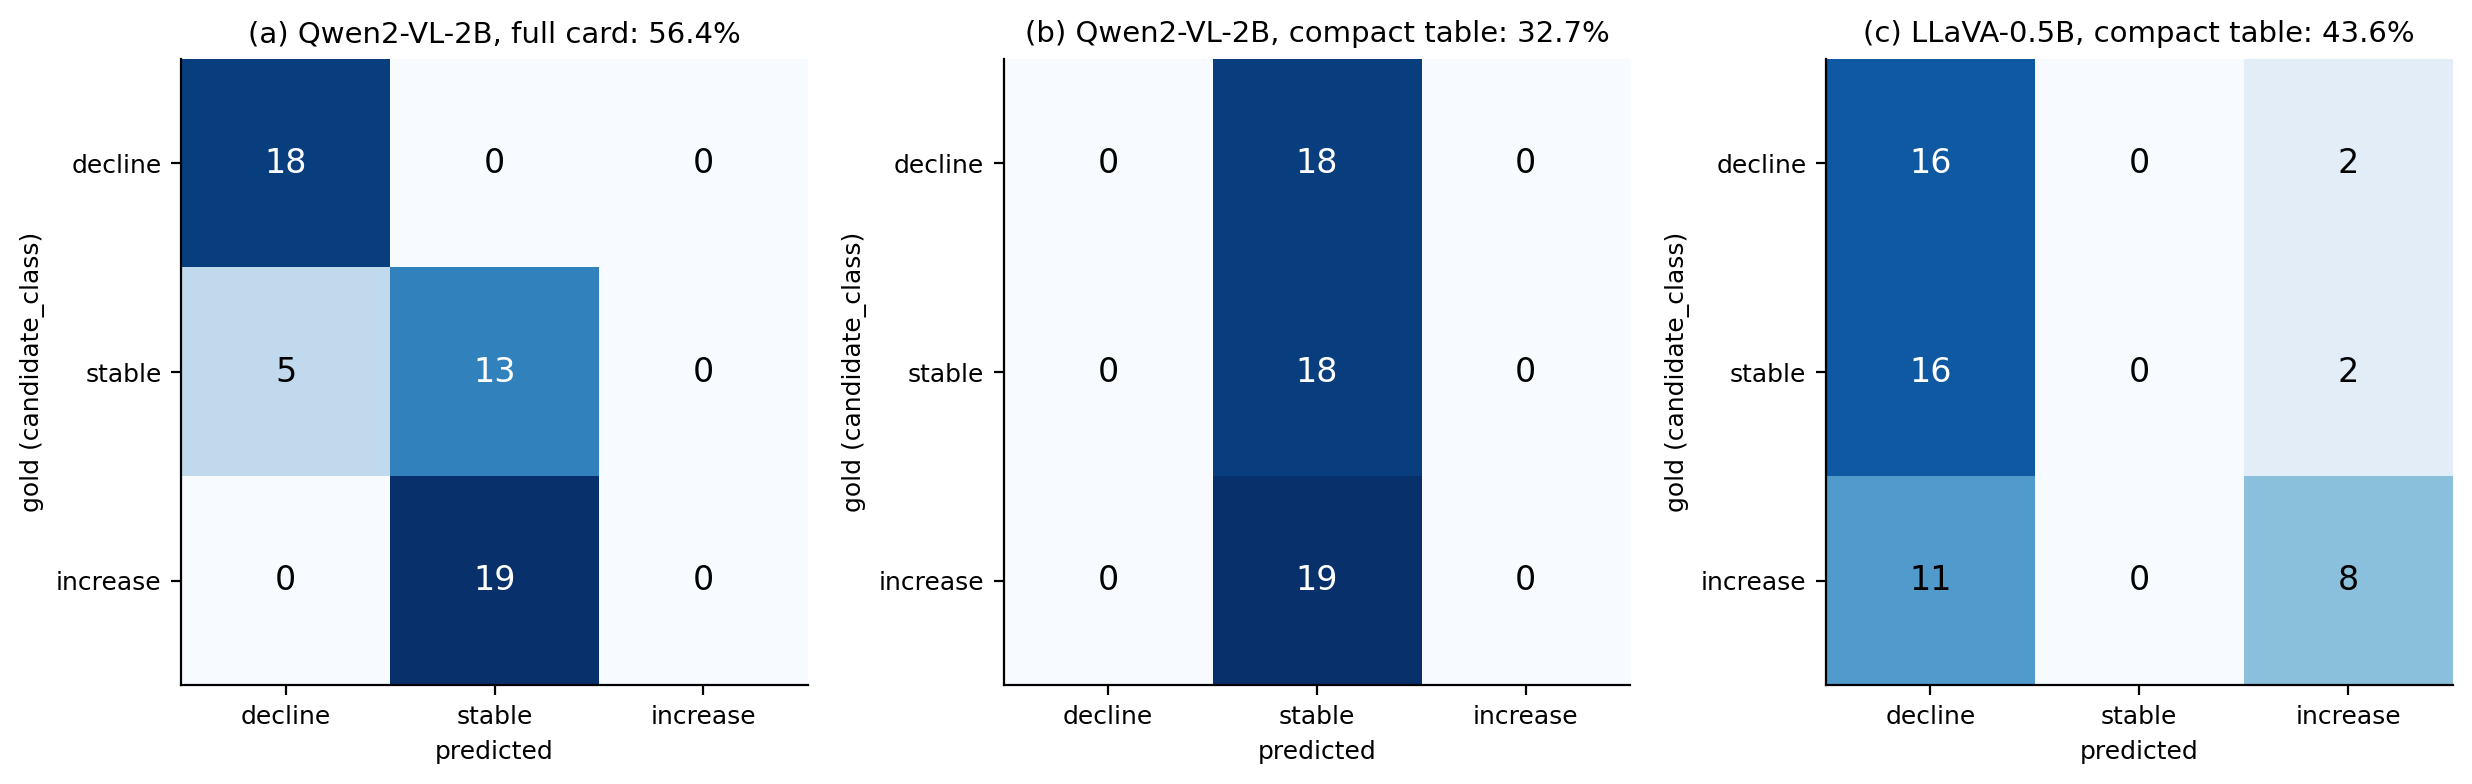
\includegraphics[width=\textwidth]{figures/fig_leakfree_confusion.png}
\caption{Confusion matrices (rows: gold; columns: predicted). (a) Qwen with the full card. (b) Qwen with the label-free compact table: ``stable'' for everything. (c) LLaVA with the compact table. Made by \file{study_guide_v3/make_figures_v3.py}.}
\label{fig:leakfreecm}
\end{figure}

\subsection{How to read them}

\begin{itemize}
  \item \textbf{Qwen's 56.4\,\% came from the summary line.} Without it Qwen falls to 32.7\,\%, the share of stable patches, because it answers ``stable'' for everything. On the patches where the two Qwen runs disagree, the full card wins 18 to 5 ($p = 0.011$): the only significant difference in Track~A.
  \item \textbf{LLaVA does better with a clean table than with the full card} (43.6\,\% against 32.7\,\%; 8 patches gained, 2 lost, $p = 0.11$), and its answers now follow the evidence somewhat: it catches most declines and some increases. But 43.6\,\% is not significantly above the 34.5\,\% baseline ($p = 0.44$), and it never answers ``stable''.
  \item \textbf{No model classifies from the evidence alone} better than guessing. This is now the central classification finding.
  \item The \texttt{compact} table and the \texttt{evidence\_only} card are different inputs (numbers only, versus the descriptive card without its last line), and Qwen scored 32.7\,\% on both.
\end{itemize}

\begin{plainwords}
With the full card, Qwen looked like the one model that could do the task. Without the card's last line it answers ``stable'' to everything. What looked like skill was the model reading a word the pipeline had already written for it. Finding this out, and saying so, is a real result of your project.
\end{plainwords}

\section{The card contains enough information}

A rule that reads one number from the card, the \dndvi{} value, and compares it with two cut-offs fitted on the training split ($-0.032$ and $-0.0011$; 96.1\,\% training accuracy) gets \textbf{52 of 55} test patches right (\textbf{94.5\,\%}, interval 85.1--98.1\,\%). With the fixed $\pm0.02$ cut-offs it gets 63.6\,\%. The rule is not a forest-change detector, since it reproduces how the labels were made, but it shows that every model in Table~\ref{tab:leakfree} had the answer in front of it as a number and did not use it.

\begin{watchout}
Another pair of cut-offs ties with this one on the training data and scores 96.4\,\% on test. Report 94.5\,\% with its cut-offs, and say how they were chosen (the first pair with the highest training accuracy).
\end{watchout}

\section{Earlier supporting analyses}

\begin{figure}[H]
\centering
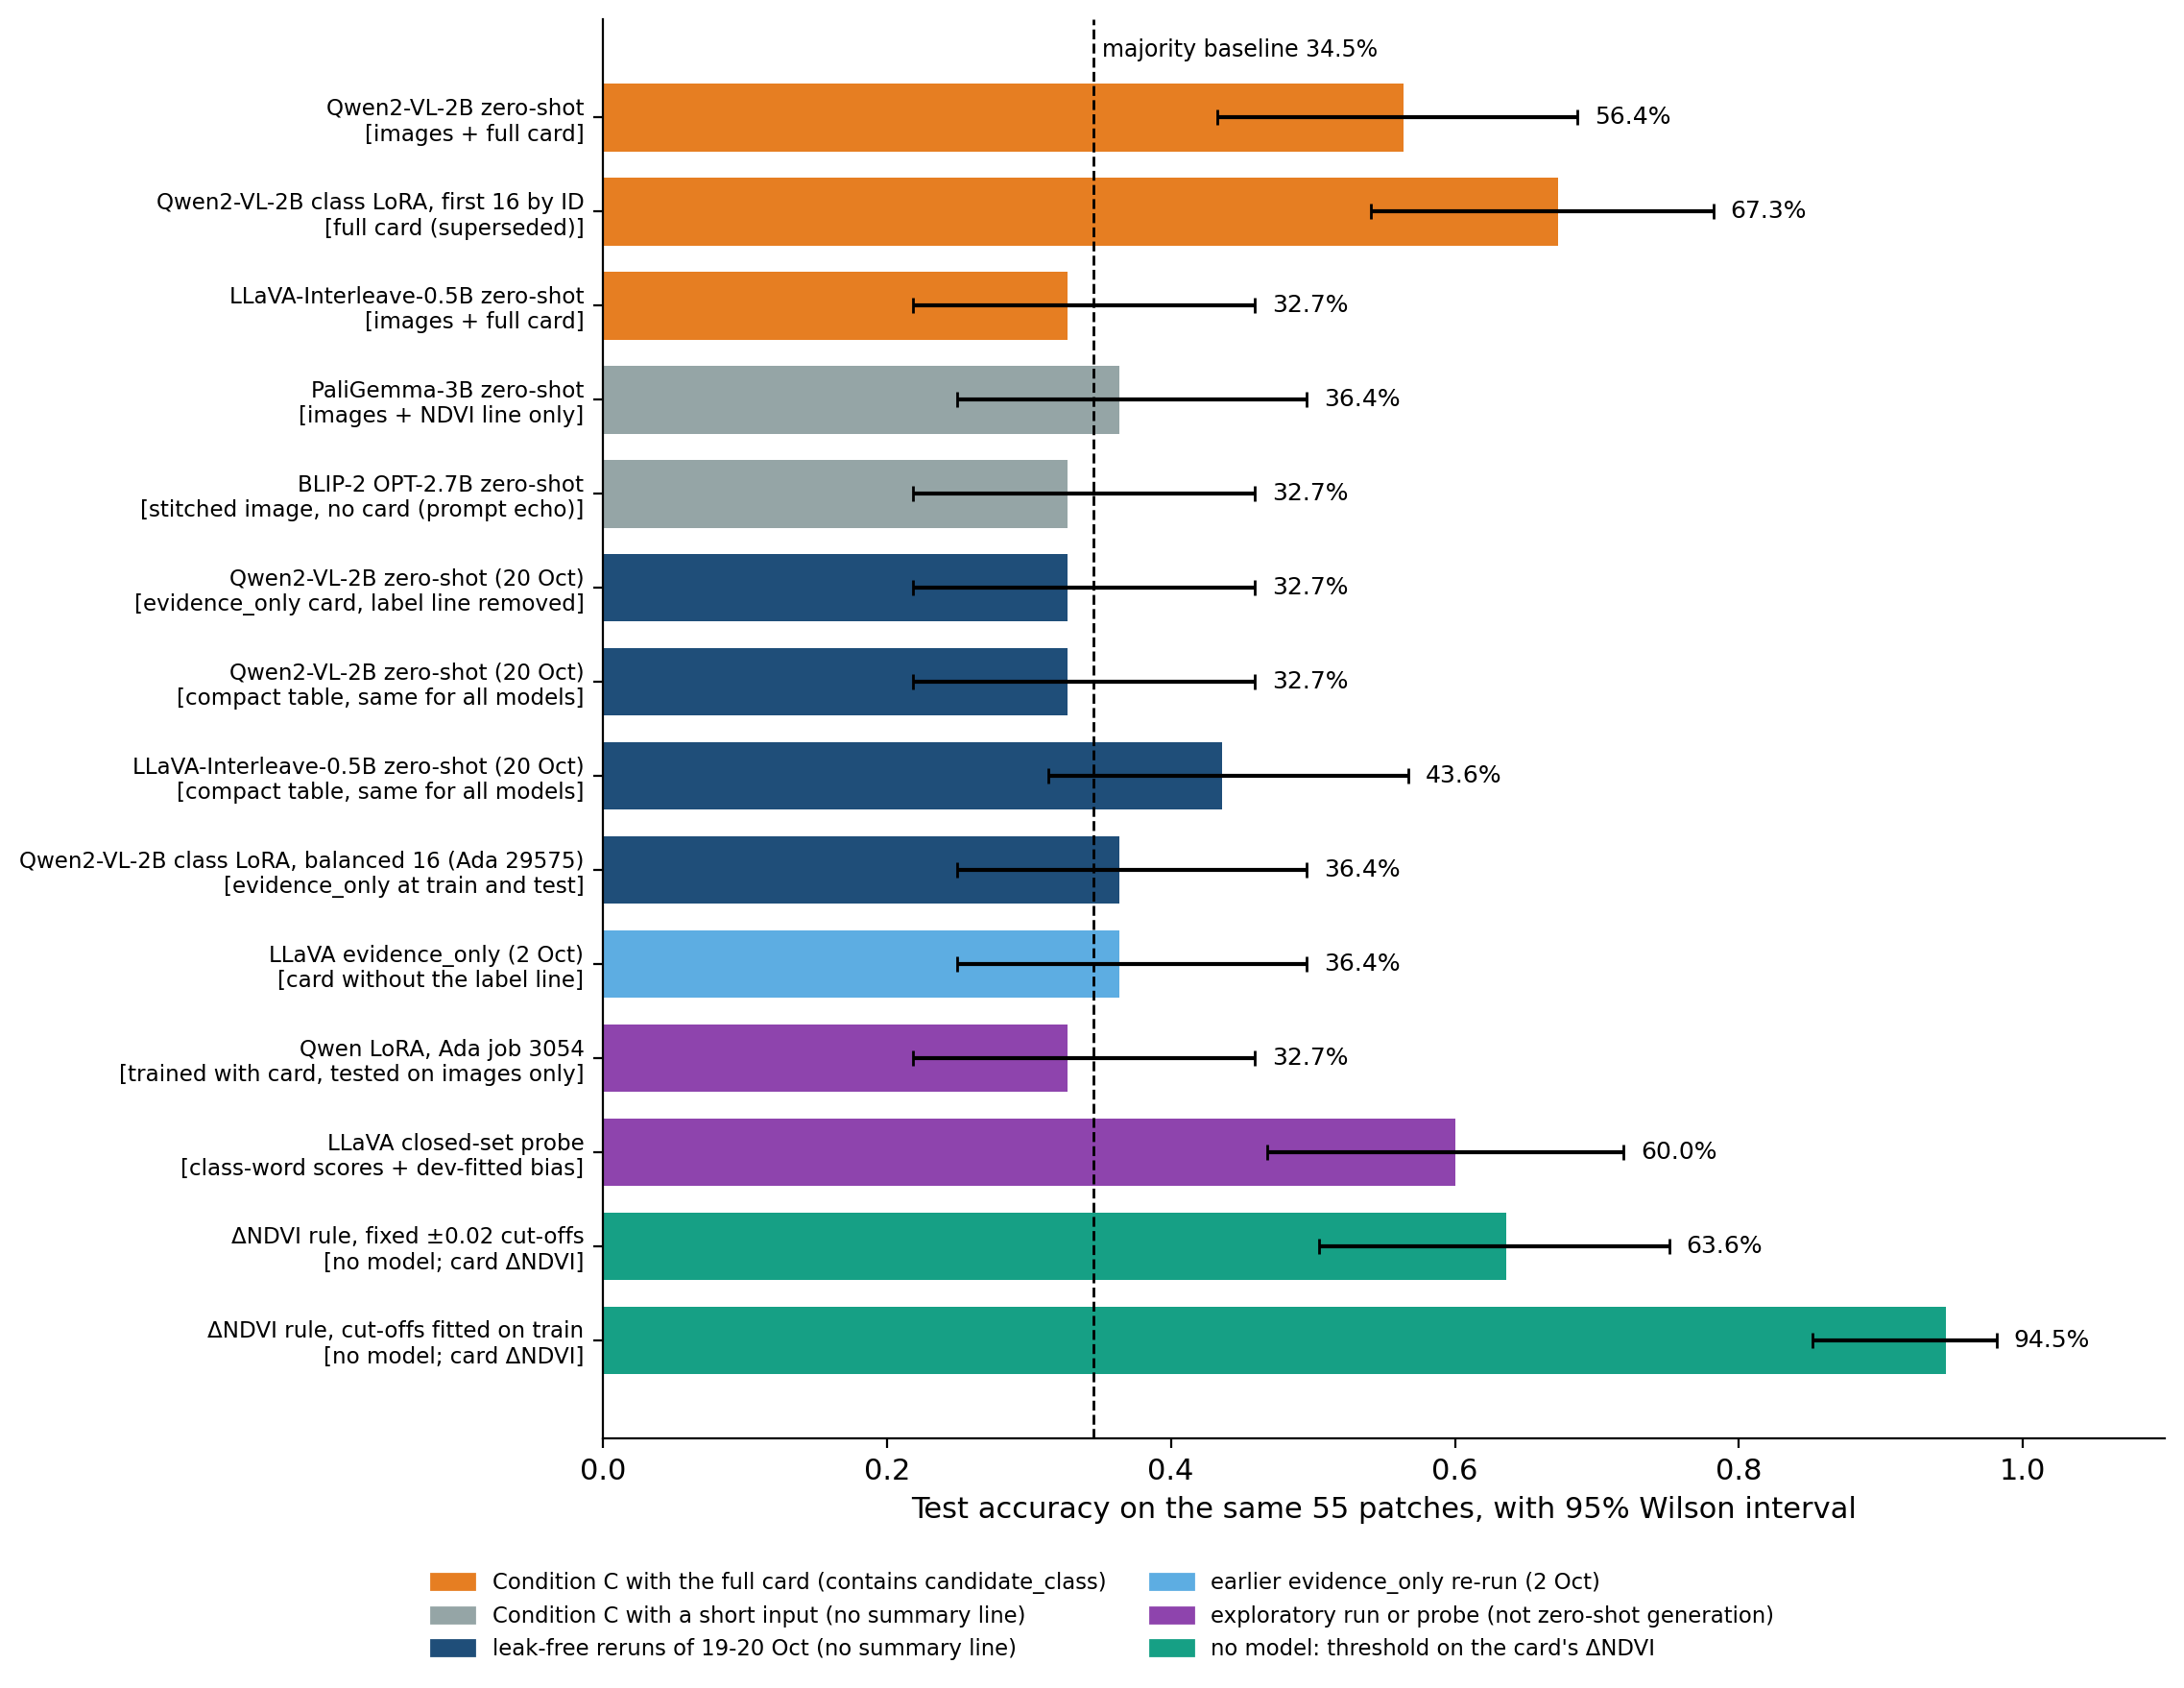
\includegraphics[width=\textwidth]{figures/fig_accuracy_v3.png}
\caption{Every classification run on the same 55 test patches, labelled by what the model was given, with 95\,\% Wilson intervals. Dark blue: the leak-free reruns of 19--20 October. Made by \file{study_guide_v3/make_figures_v3.py}.}
\label{fig:accv2}
\end{figure}

\paragraph{The 2 October \texttt{evidence\_only} re-run.} LLaVA 36.4\,\%, PaliGemma 36.4\,\% and BLIP-2 32.7\,\% (\file{results/explain/oneword_*.json}). Only LLaVA's input changed; PaliGemma and BLIP-2 never had the line. This run is now superseded by the Phase~E reruns, which also cover Qwen.

\paragraph{The closed-set probe.} \file{src/vlm_closedset.py} (Ada, 2 October) scores each class word's likelihood with a four-panel image, a prompt stating the $\pm0.02$ rule, and three biases fitted on the development set. LLaVA reached 60.0\,\% (33/55) but never answered ``stable'' and matched the stated rule on only 25 patches; PaliGemma and BLIP-2 answered ``stable'' for everything (32.7\,\%). It is a probe with a tuned bias, not a zero-shot result.

\paragraph{The exploratory Ada fine-tune tested on images only} (job 3054, 32.7\,\%) belongs to Track~B (Chapter~\ref{ch:trackB}).

\begin{figure}[H]
\centering
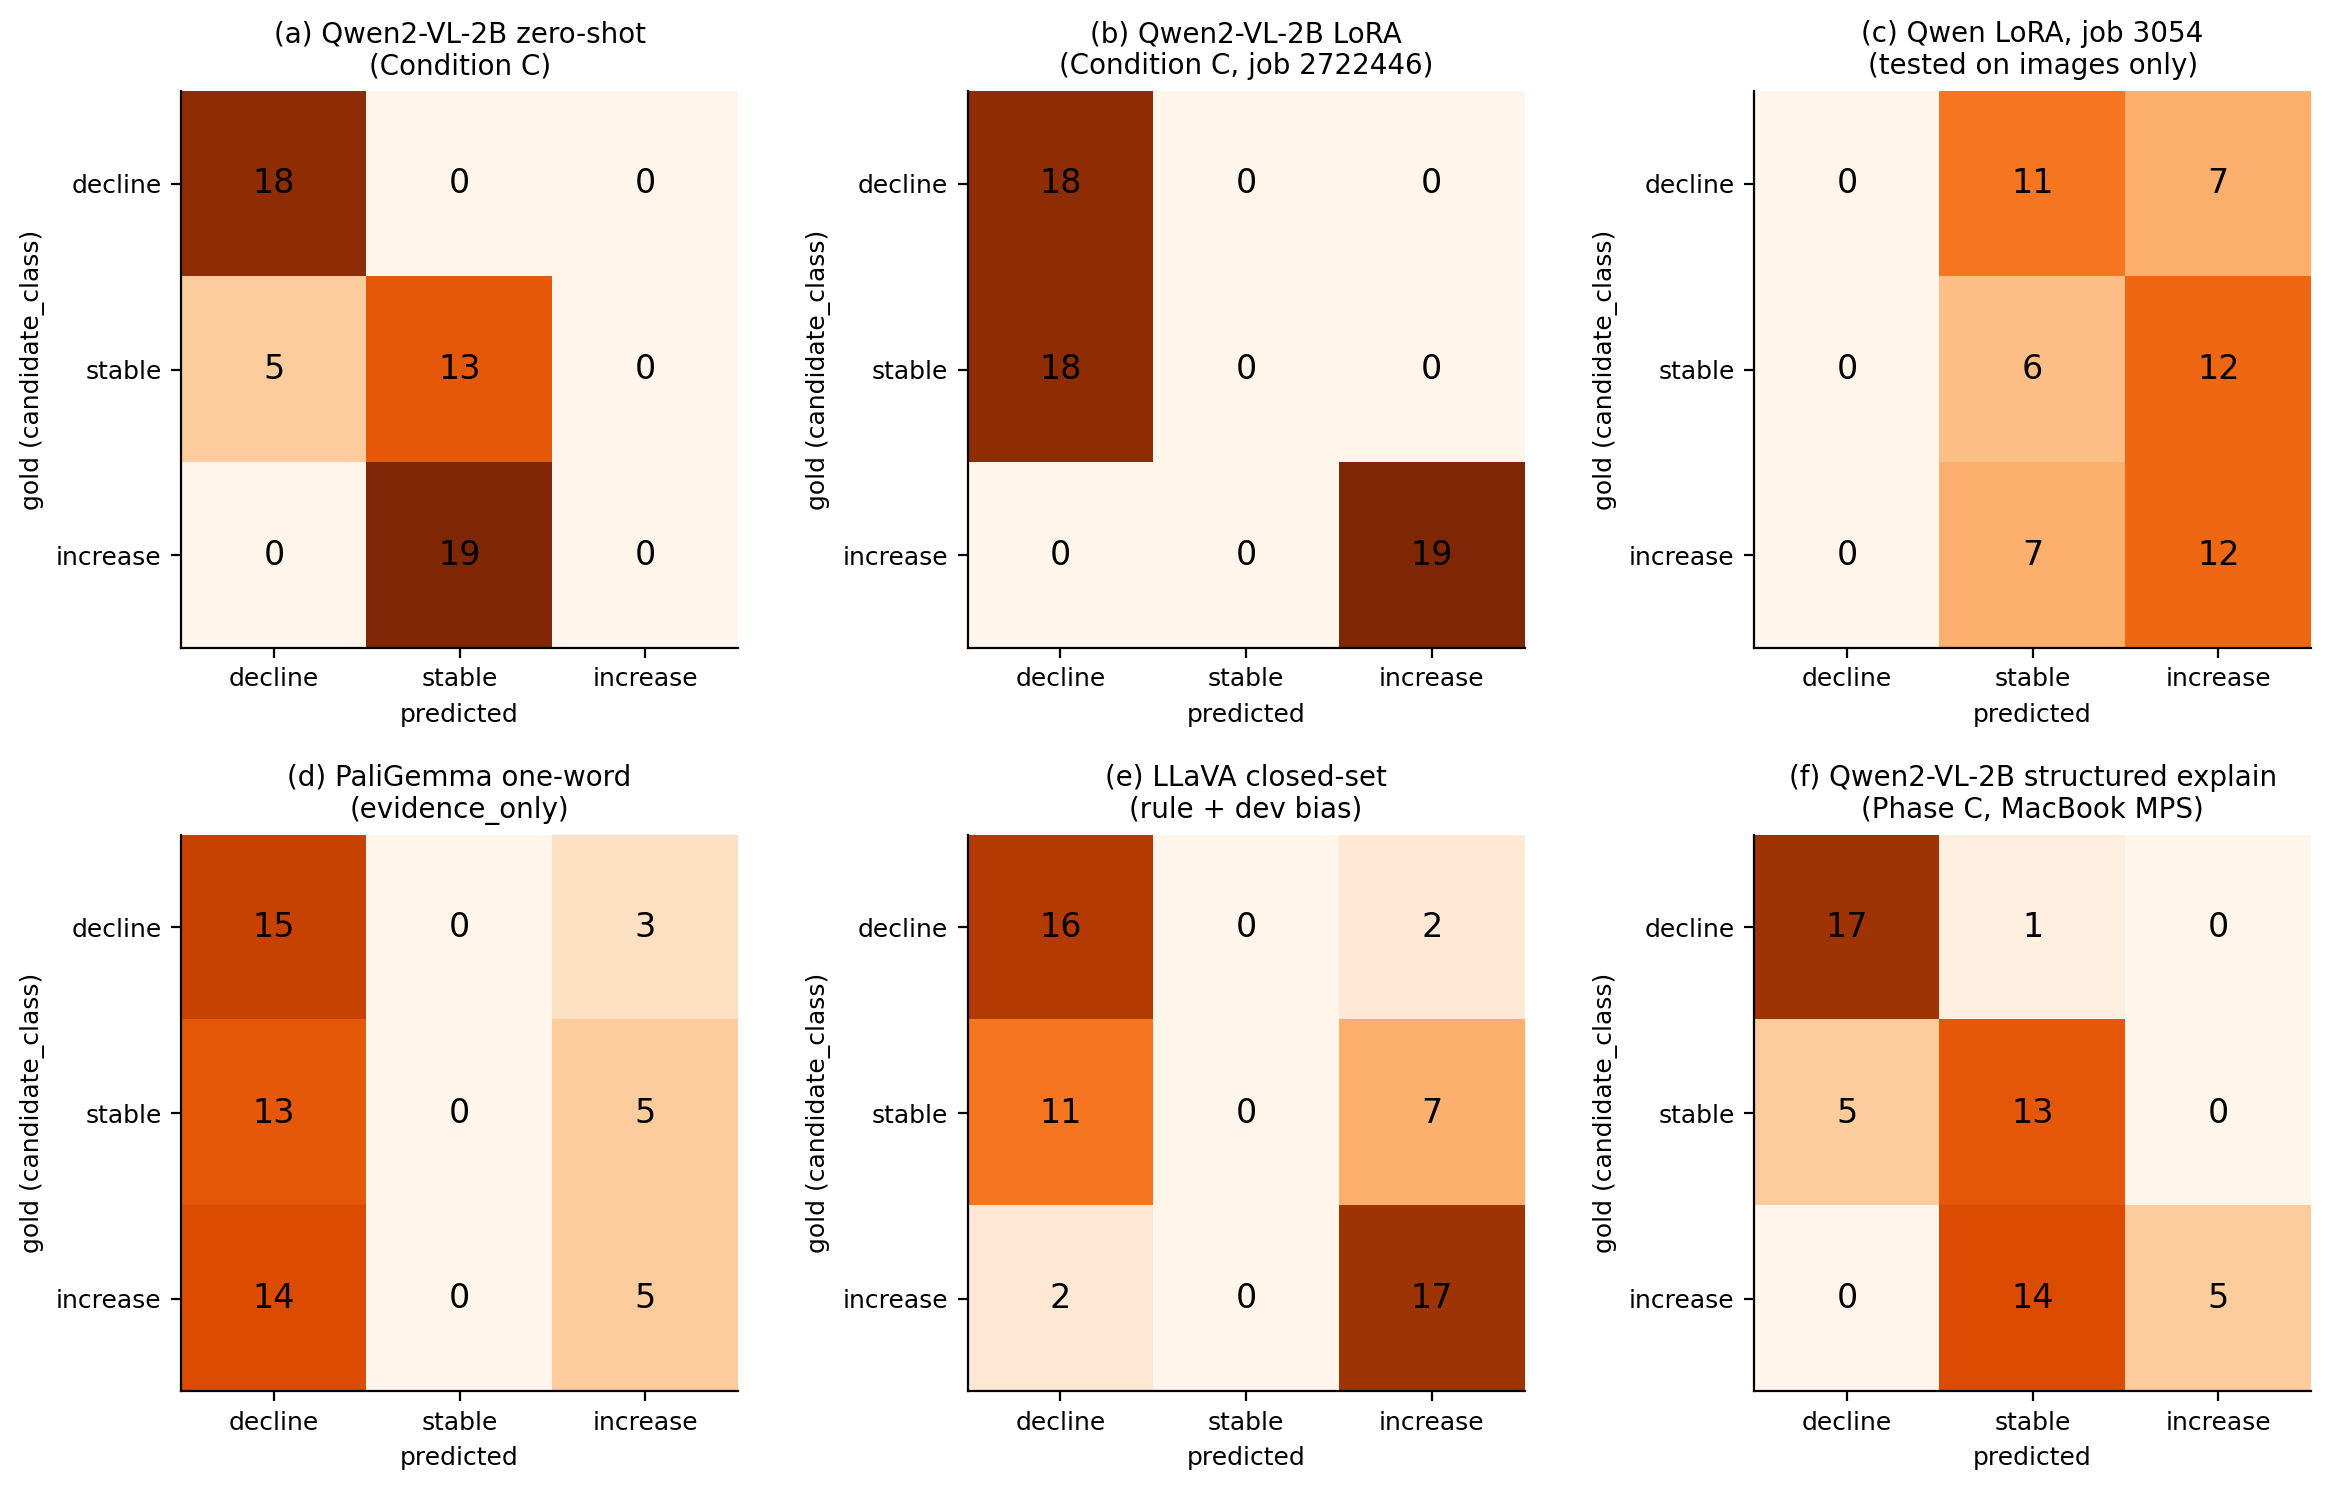
\includegraphics[width=\textwidth]{figures/fig_confusion.png}
\caption{Confusion matrices from the first two phases. (a) Qwen zero-shot and (b) the old Qwen class LoRA, both with the full card; (c) an exploratory fine-tune tested on images only; (d) PaliGemma with the summary line removed (its input was in fact unchanged); (e) the closed-set LLaVA probe; (f) Qwen with the structured explanation prompt.}
\label{fig:confusionA}
\end{figure}

\section{How this compares with other work}

\begin{itemize}
  \item Established forest-change methods work directly on spectral numbers and time series: global forest-loss maps \citep{hansen2013}, LandTrendr \citep{kennedy2010}, CCDC \citep{zhu2014}, radar alerts \citep{reiche2021}, and change-detection networks trained on image pairs \citep{daudt2018}. The threshold baseline is a minimal version of that approach, and it wins easily.
  \item Remote-sensing VLMs and datasets, such as GeoChat \citep{kuckreja2024}, remote-sensing question answering \citep{lobry2020} and change captioning \citep{liu2022levircc}, depend on large remote-sensing training sets. The models here were trained mainly on everyday photographs, and the forest chips are dark and nearly identical between years (Figure~\ref{fig:examples}).
\end{itemize}

\begin{figure}[H]
\centering
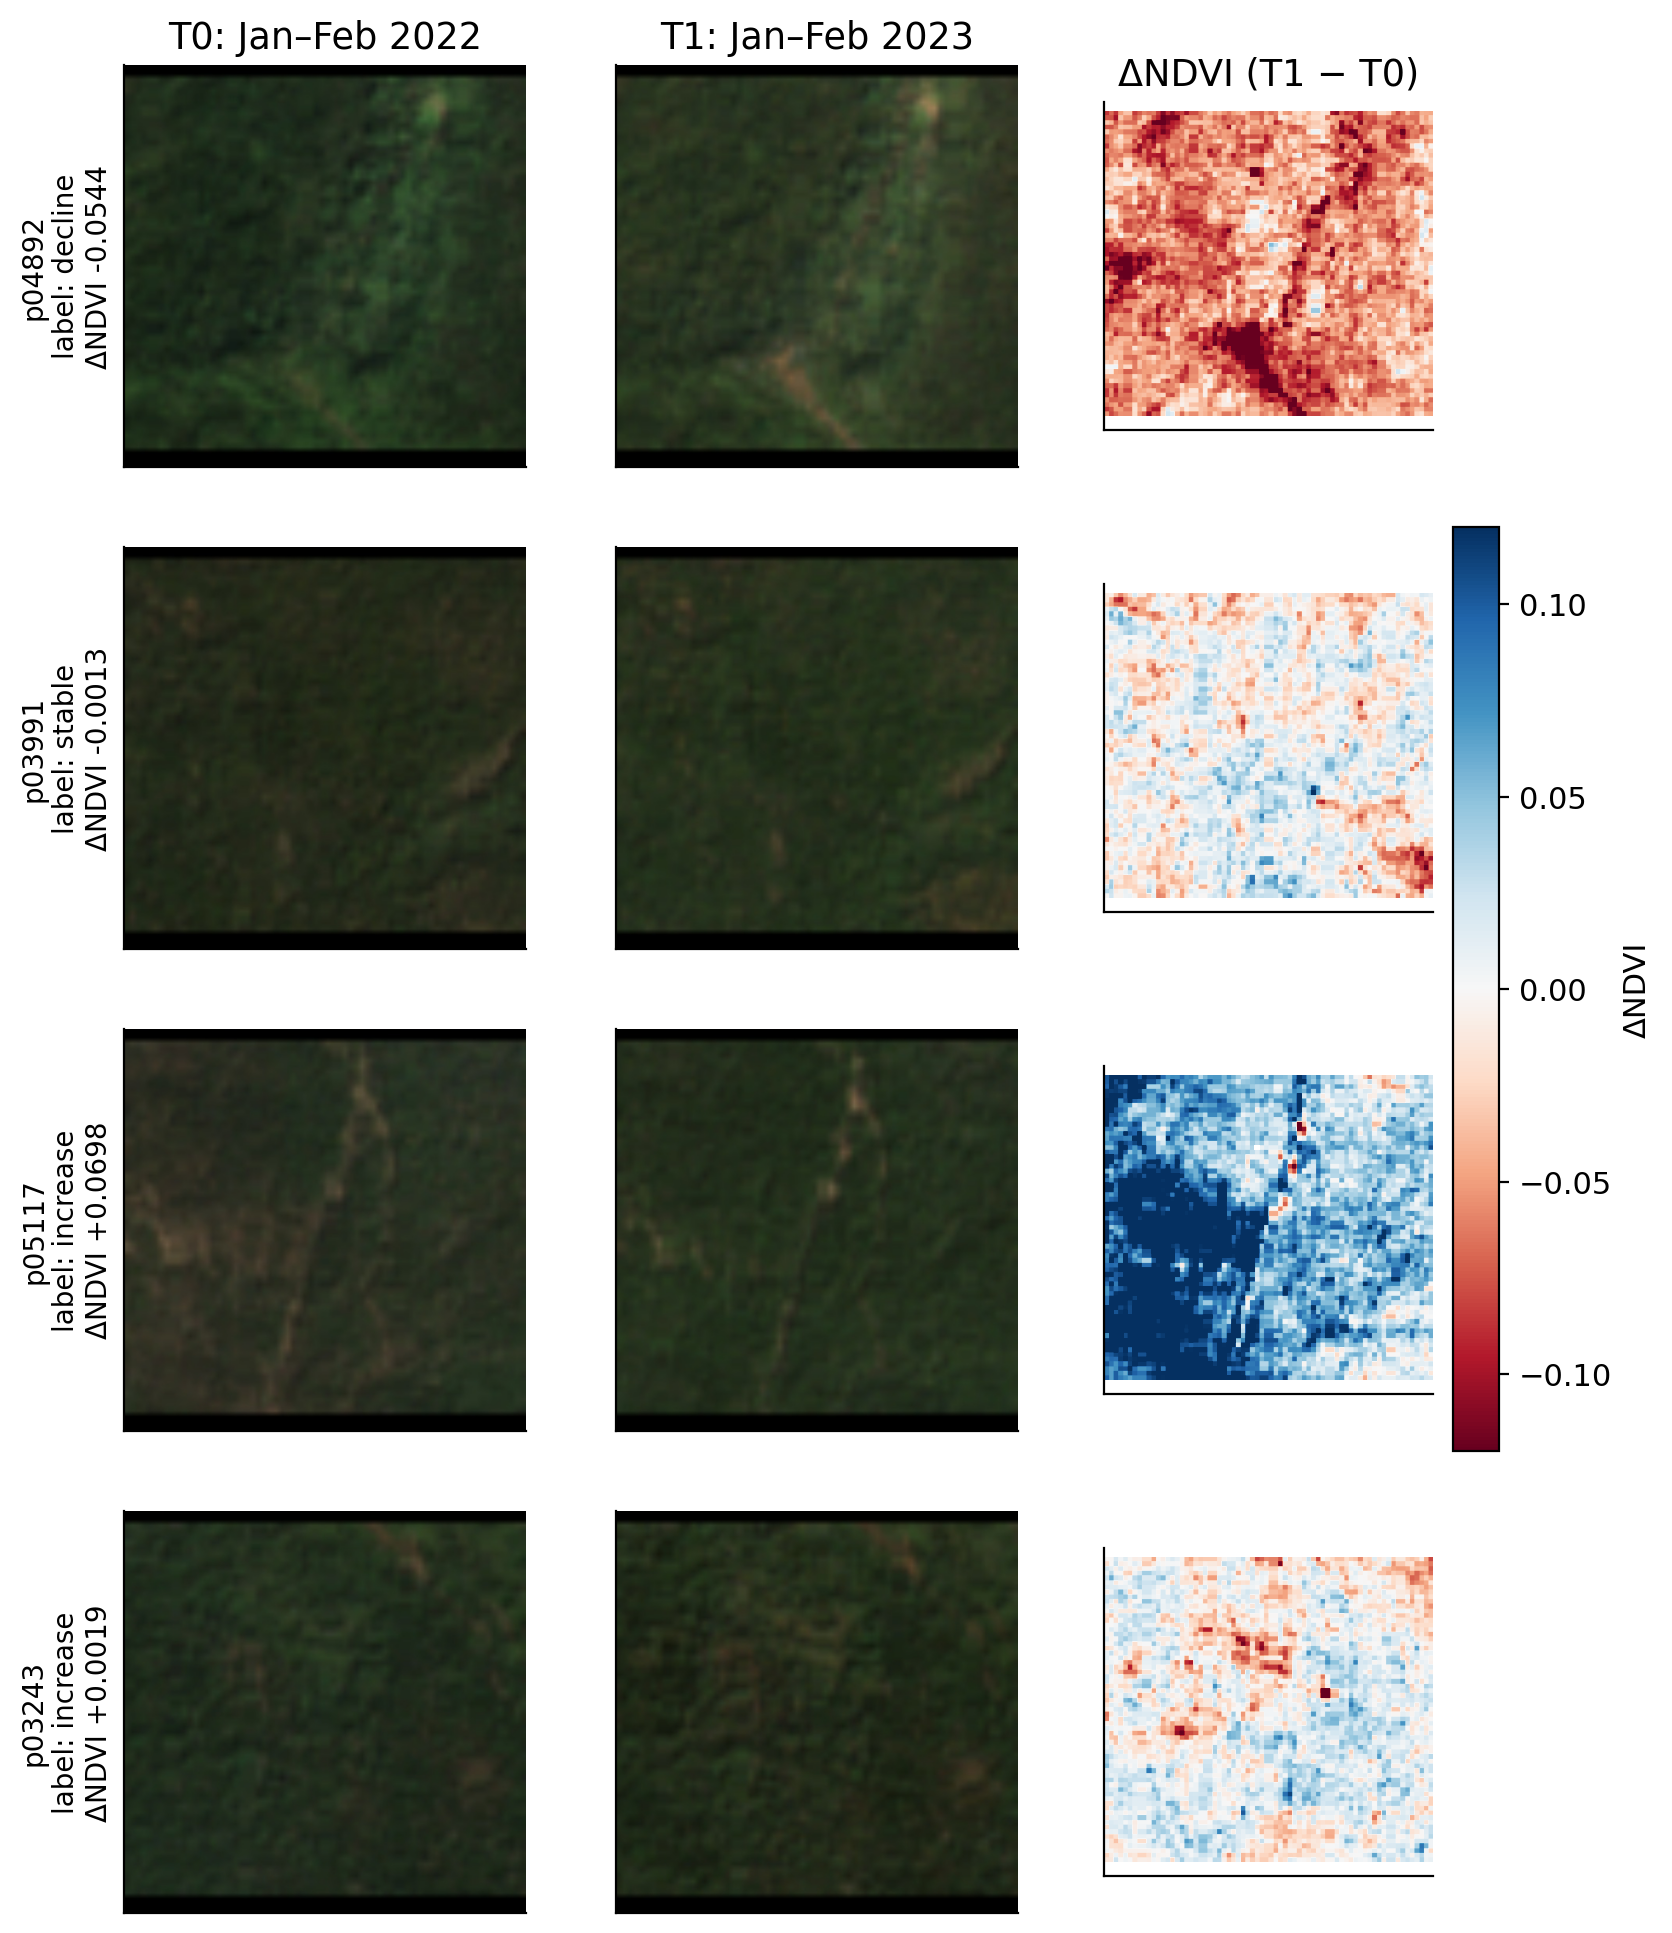
\includegraphics[width=0.78\textwidth]{figures/fig_examples.png}
\caption{Four test patches: the largest NDVI drop among test decline patches (p04892), a typical stable patch (p03991), the largest gain among test increase patches (p05117), and the smallest gain labelled increase (p03243). The \dndvi{} maps show the change clearly; the colour pairs mostly do not. Black bands are padding.}
\label{fig:examples}
\end{figure}

\begin{foryourreport}
In ``Zero-Shot Model Performance'' (about 700 words):
\begin{itemize}
  \item One table in two blocks (Chapter~\ref{ch:results}): the leak-free runs first (Table~\ref{tab:leakfree}), then the full-card runs (Table~\ref{tab:trackA}), each with an \emph{Input} column, intervals and the baselines.
  \item The summary line: what it contains (trend word and label) and what removing it does to Qwen (56.4\,\% $\rightarrow$ 32.7\,\%, $p = 0.011$). Figure~\ref{fig:leakfreecm} shows it at a glance.
  \item LLaVA's 43.6\,\% with the equal-input table, and why it is not significant.
  \item Why PaliGemma and BLIP-2 have no leak-free score (gated model; no parsable answers), and that BLIP-2's earlier 32.7\,\% was an echo.
  \item The 94.5\,\% threshold baseline: the information was on the card.
  \item Do \emph{not} write that Qwen ``did not copy the label'' as evidence for its skill (Section~\ref{sec:summaryline}).
\end{itemize}
\end{foryourreport}

\begin{selfcheck}
\begin{enumerate}
  \item What two pieces of information does the summary line carry?
  \item Why was version~2's claim that Qwen's 56.4\,\% ``did not come from copying'' misleading?
  \item What did Qwen answer once the summary line was removed, and what accuracy does that give?
  \item Is LLaVA's 43.6\,\% evidence that it can classify? Give two reasons for your answer.
  \item Why do PaliGemma and BLIP-2 have no leak-free result?
  \item What does the 94.5\,\% threshold rule show about the models?
\end{enumerate}
\end{selfcheck}

\chapter{Track B: the class LoRA}
\label{ch:trackB}

Track~B asks: \emph{does a small amount of task-specific training change what Qwen2-VL-2B can do?} It was first run on 29 September with the full card (67.3\,\%), and re-run properly on 20 October with balanced training patches and the label-free card (36.4\,\%). The second run is the one to report.

\section{The reported run: balanced and leak-free (Ada job 29575)}

\begin{wherecode}
\file{scripts/ada_slurm_qwen_balanced_smoke.sh} on Ada (job 29575, finished 20 October 03:34), using \file{scripts/run_finetune_qwen.py} with \texttt{--balanced-train} and \texttt{--eval-prompt evidence\_only}. Log: \file{results/slurm-qwen-balanced-smoke-29575.log}. Result: \file{results/protocol/qwen_balanced_leakfree_lora.json} (copied from Ada).
\end{wherecode}

\begin{table}[H]
\centering
\caption{The reported class-LoRA run.}
\label{tab:classlora}
\small
\begin{tabularx}{\textwidth}{lY}
\toprule
Base model & \texttt{Qwen/Qwen2-VL-2B-Instruct}, stored in 4 bits (NF4) \\
Adapter & LoRA, $r = 8$, $\alpha = 16$, dropout 0.1, attention and MLP projections \\
Optimiser & AdamW, learning rate $5\times10^{-5}$, weight decay 0.05 \\
Effective batch & 1 example $\times$ 4 accumulation steps \\
Training data & 16 training patches drawn evenly by class (seed 42): \textbf{6 decline, 5 stable, 5 increase} \\
Input at training and test & both images and the \texttt{evidence\_only} card (summary line removed) \\
Target & \texttt{\{"change\_class": "<label>"\}}; loss on the answer tokens only \\
Epochs & 1 (mean training loss 2.73); development accuracy 34.5\,\% \\
Test & the same 55 test patches, one-word answer \\
\bottomrule
\end{tabularx}
\end{table}

\subsection{The result}

\textbf{36.4\,\%} (20 of 55; 95\,\% interval 24.9--49.6\,\%; macro-F1 0.236). The adapter answered ``stable'' for 53 of the 55 patches: all 18 stable patches right, 2 of 18 decline patches right, 0 of 19 increase patches right (Figure~\ref{fig:loraclasses}c).

\begin{plainwords}
Once the label line is gone, a 16-example, one-epoch LoRA does not teach the model the task. It learns to say ``stable'' almost every time, which scores about the same as always saying ``increase'' (McNemar $p = 1.0$) and barely differs from zero-shot Qwen without the label line, which in its \texttt{compact} run said ``stable'' to everything ($p = 0.50$; the inputs differ slightly, card versus table).
\end{plainwords}

\begin{figure}[H]
\centering
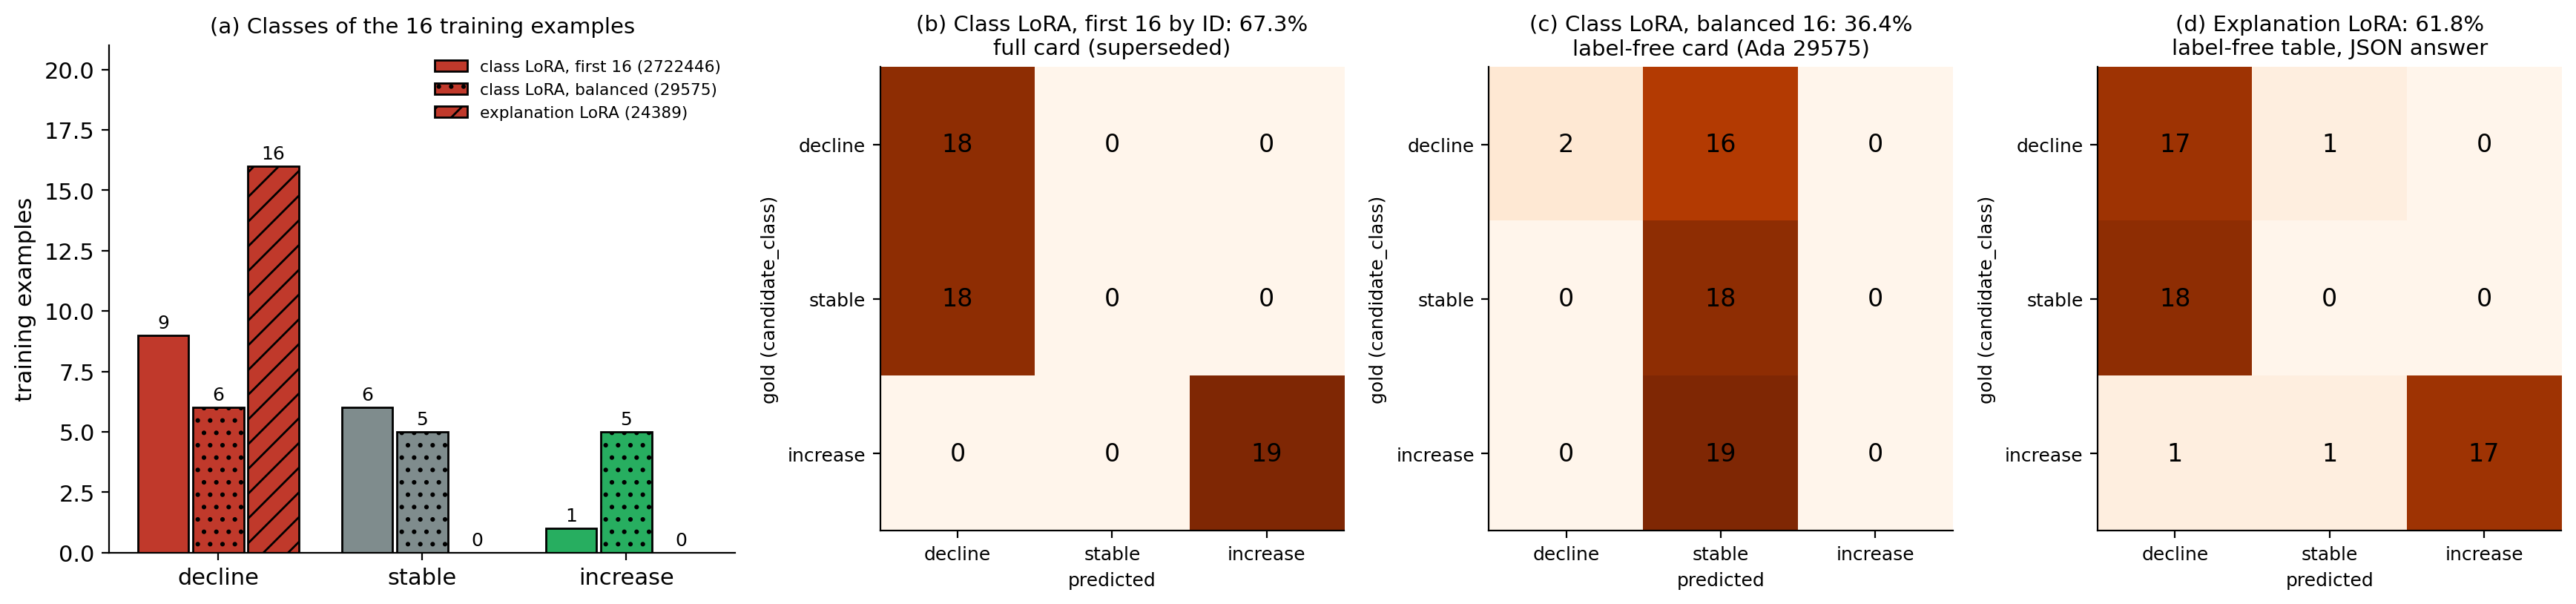
\includegraphics[width=\textwidth]{figures/fig_lora_v3.png}
\caption{All three LoRA runs. (a) Classes of the 16 training examples. (b) The first class LoRA (first 16 patches by ID, full card): 67.3\,\%, superseded. (c) The balanced, leak-free class LoRA: 36.4\,\%. (d) The explanation LoRA (Chapter~\ref{ch:trackC}). Made by \file{study_guide_v3/make_figures_v3.py}.}
\label{fig:loraclasses}
\end{figure}

\section{The first run, now superseded (Ada job 2722446)}

The first class LoRA (29 September, \texttt{--max-train 16 --epochs 1}) used the full card at training and test, and its 16 patches were simply the first 16 training patches by ID: 9 decline, 6 stable and 1 increase. It reached \textbf{67.3\,\%} (37/55): all decline and all increase patches right, every stable patch called ``decline'' (Figure~\ref{fig:loraclasses}b). It recognised all 19 increase patches from a single increase example, including 10 whose card trend word says ``stable'': on those cards only the \dndvi{} numbers and the summary line's \texttt{candidate\_class=increase} say ``increase''. Set beside job 29575, the likeliest reading is that it learned to use the label line.

\begin{newinfo}
Cite 36.4\,\% as your class-LoRA result. Keep 67.3\,\% only in an appendix or a single sentence, described as ``an earlier run on 16 unbalanced patches with the full card, which contains the label line''. Do not call it a leak-free or balanced result.
\end{newinfo}

\section{All fine-tuning jobs}

\begin{table}[H]
\centering
\caption{Every class-LoRA job whose log was copied back (\file{ada_review/EcoExplain-VLM-results/slurm-qwen09-*.log}, \file{results/slurm-qwen-balanced-smoke-29575.log}). Job 2722478 planned 3 epochs and its log ends after the first (loss 0.13); job 2792 stopped early after 2 epochs; jobs 2984 and 3054 had development accuracy 34.5\,\%. Job 2856 left an empty log. An earlier balanced job (29571) also finished; your notes name 29575 as the final artifact, and only its log is in the project.}
\label{tab:ftruns}
\small
\begin{tabular}{llrrlrr}
\toprule
Job & Date & Train & Epochs & Input (train / test) & Final loss & Test acc. \\
\midrule
\textbf{29575 (reported)} & 20 Oct & 16 bal. & 1 & label-free / label-free & 2.73 & \textbf{36.4\,\%} \\
2722446 (superseded) & 29 Sep & 16 by ID & 1 & full card / full card & 1.84 & 67.3\,\% \\
2722478 & 29 Sep & 256 & 1 of 3 & full card / --- & 0.13 & log ends \\
2690 & 2 Oct & 256 & 3 & full card / full card & 0.0000 & 100\,\% \\
2792 & 2 Oct & 256 & 2 & full card / full card & 0.0001 & 100\,\% \\
2984 & 2 Oct & 128 & 1 & full card / images only & 0.87 & 32.7\,\% \\
3054 & 2 Oct & 128 & 1 & full card / images only & 0.91 & 32.7\,\% \\
\bottomrule
\end{tabular}
\end{table}

\begin{itemize}
  \item \textbf{Jobs 2690 and 2792 reached 100\,\%} with almost zero training loss: with 256 examples and the full card, the model learned that the answer is written in the card's last line. Excluded.
  \item \textbf{Jobs 2984 and 3054} were trained with the card and tested on images alone: 32.7\,\%. Training and test inputs differ, so this is not a clean measurement.
  \item \textbf{Job 29575} is the first run in which training and test both lack the label line and the training classes are balanced. It is the only class-LoRA number that measures what the research question asks.
\end{itemize}

\begin{whybox}
Why still only 16 patches and one epoch? Job 29575 repeats the size of the first run so that the two differ only in balance and input, and it fits Ada's quota and queue. The natural next step is the configuration already scripted in \file{docs/PROTOCOL_RERUN.md}: 48 balanced patches (16 per class), or all 256, with the label-free card and early stopping on the development set.
\end{whybox}

\section{What you can and cannot claim}

\begin{table}[H]
\centering
\small
\begin{tabularx}{\textwidth}{YY}
\toprule
\textbf{You can say} & \textbf{You should not say} \\
\midrule
A LoRA on 16 balanced patches for one epoch, without the label line, reached 36.4\,\%, answering ``stable'' for 53 of 55 patches. & ``Fine-tuning improved the model to 67.3\,\%.'' \\
This is not better than always guessing one class ($p = 1.0$). & ``LoRA fixed the model's weaknesses.'' \\
An earlier unbalanced run with the full card reached 67.3\,\%, and longer full-card runs 100\,\%, because the card states the label. & ``The model reached 100\,\% after more training.'' \\
Larger, balanced, label-free fine-tuning remains untested. & ``Fine-tuning does not work for this task'' (16 examples cannot show that). \\
\bottomrule
\end{tabularx}
\end{table}

\begin{foryourreport}
In ``Effect of Fine-Tuning'' (about 400 words):
\begin{itemize}
  \item The configuration (Table~\ref{tab:classlora}), including the 6/5/5 balanced sample and the label-free card.
  \item 36.4\,\% with its interval, the per-class pattern (``stable'' for 53 of 55) and the McNemar tests.
  \item The earlier 67.3\,\% and 100\,\% runs in two sentences, as the reason the protocol was changed; Table~\ref{tab:ftruns} in an appendix.
  \item What would be needed next (more balanced patches, early stopping).
\end{itemize}
\end{foryourreport}

\begin{selfcheck}
\begin{enumerate}
  \item How did the training data and the input of job 29575 differ from those of job 2722446?
  \item What did the balanced, leak-free adapter answer, and why is 36.4\,\% not evidence of learning?
  \item Why is 67.3\,\% no longer the result to cite?
  \item What do jobs 2690 and 2792 show, and why are they excluded?
  \item What experiment would test fine-tuning properly?
\end{enumerate}
\end{selfcheck}

\chapter{Track C: explanations}
\label{ch:trackC}

Track~C asks the second half of the research question: \emph{when a model gives a class, is its justification supported by the evidence?} It was tried three ways, in three phases:

\begin{enumerate}
  \item \textbf{Phase B, free-form prompt} (2--3 October, laptop): ``explain in your own words''.
  \item \textbf{Phase C, structured cite-only prompt} (6 October, MacBook Air GPU): ``copy listed facts and follow a stated rule''.
  \item \textbf{Phase D, explanation LoRA} (16--17 October, Ada): fine-tune Qwen2-VL-2B on 16 of its own filtered justifications.
\end{enumerate}

In all three the label is \emph{removed} from the input, and every claim is checked automatically against the measured changes (Section~\ref{sec:scorer}).

\section{What the models receive in explanation mode}

Instead of the long card, each model gets a compact table of numbers with no class words and no interpretive words (\texttt{compact\_evidence} in \file{src/vlm_evidence.py}). For p00575:

\begin{tcolorbox}[colback=gray!4,colframe=gray!50,fontupper=\scriptsize\ttfamily]
Evidence (T0 2022 -> T1 2023, patch means):\\
NDVI 0.625 -> 0.575 ($\Delta$ -0.050); 48.9\% of pixels dropped by more than 0.05\\
EVI $\Delta$ -0.004 | NDMI $\Delta$ -0.007 | NBR $\Delta$ +0.003\\
Green cover in RGB 0.74 -> 0.42\\
SAR VV $\Delta$ -0.22 dB, VH $\Delta$ -0.41 dB\\
Rainfall Jan--Feb 72.5 -> 25.4 mm\\
Soil moisture anomaly +0.027 -> -0.048 | Temperature anomaly -1.5 -> +1.1 \textdegree C\\
Elevation 834 m, slope 5\textdegree
\end{tcolorbox}

\file{scripts/check_no_leak.py} confirms that no explanation prompt contains \texttt{candidate\_class}. The numbers come from the card, so they carry the padding bias of Chapter~\ref{ch:stage03}.

\section{Phase B: the free-form prompt}

\subsection{The instruction}

Qwen and LLaVA received (\texttt{EXPLAIN\_JSON\_ASK} in \file{src/vlm_eval.py}):

\begin{tcolorbox}[colback=gray!4,colframe=gray!50,fontupper=\scriptsize]
Image 1 is a forest patch in Jan--Feb 2022, image 2 is the same patch in Jan--Feb 2023. First describe in one sentence what visibly changed between the two images. Then decide whether vegetation is stable, declined, or increased. Justify your decision in 2--3 sentences in your own words, citing the specific numbers that support it, and mention any evidence that contradicts it. If climate (rainfall, soil moisture, temperature) could explain the change, say so as a possibility, not a certainty. Do not repeat the table. Answer as JSON: \{"visual\_change", "change\_class", "justification", "supporting\_evidence", "conflicting\_evidence", "possible\_driver", "confidence"\}
\end{tcolorbox}

PaliGemma and BLIP-2 cannot follow long JSON instructions, so they received only the NDVI line and ``Left image is 2022, right image is 2023. class: stable or decline or increase. reason: one sentence.''

\begin{whybox}
The table holds no class words and the prompt asks for reasoning ``in your own words'', so a model cannot score well by copying the dataset's narrative. Asking for supporting \emph{and} contradicting evidence follows the roadmap's structured-explanation condition; asking for drivers ``as a possibility'' tests causal restraint.
\end{whybox}

\subsection{What happened}

\begin{table}[H]
\centering
\caption{Phase~B scores (\texttt{scripts/score\_explanations.py --include-legacy}; files \file{results/explain/explain_*.json}). Qwen was run on 3 patches only.}
\label{tab:phaseB}
\small
\begin{tabular}{lrrrr}
\toprule
 & Qwen2-VL-2B & LLaVA-0.5B & PaliGemma-3B & BLIP-2 \\
\midrule
Patches explained & 3 & 55 & 55 & 55 \\
Class accuracy & 3 of 3 & 29.1\,\% & 33.3\,\% of 36 & 32.7\,\% \\
Checkable claims per explanation & 5.33 & 1.09 & 0 & 0 \\
Correct claims & 7/16 (43.8\,\%) & 34/60 (56.7\,\%) & --- & --- \\
With $\ge 1$ wrong claim & 3/3 & 19/55 (34.5\,\%) & --- & --- \\
Self-consistency & 66.7\,\% & 10.3\,\% & --- & --- \\
Distinct-2 & 0.685 & 0.069 & 0.000 & 0.018 \\
Near-duplicate share & 0 & 34.5\,\% & 100\,\% & 100\,\% \\
\bottomrule
\end{tabular}
\end{table}

\begin{description}
  \item[PaliGemma] answered ``decline'' 36 times and ``unanswerable'' 19 times, never with a reason.
  \item[BLIP-2] returned its prompt for all 55 patches; the echo contained ``class: stable or decline or increase'', so every answer was parsed as ``stable''. No explanation exists.
  \item[LLaVA] wrote fluent paragraphs, often in loops (``The first image has a green color with no visible changes \dots'' repeated, alternating ``increase'' and ``decrease''). Just over half of its checkable claims were right, and its claims rarely pointed the same way as its own class (10.3\,\%).
  \item[Qwen] gave readable JSON that cited numbers, but only 3 patches were run (a dry-run setting). Its ``visual change'' field copied numbers instead of describing the images, it reported \texttt{"confidence": 0.0} every time, and for p00086 it attributed the change to ``the increase in rainfall'' when rainfall fell from 62.5 to 22.4\,mm: a factual error and an unsupported causal claim in one.
\end{description}

\begin{figure}[H]
\centering
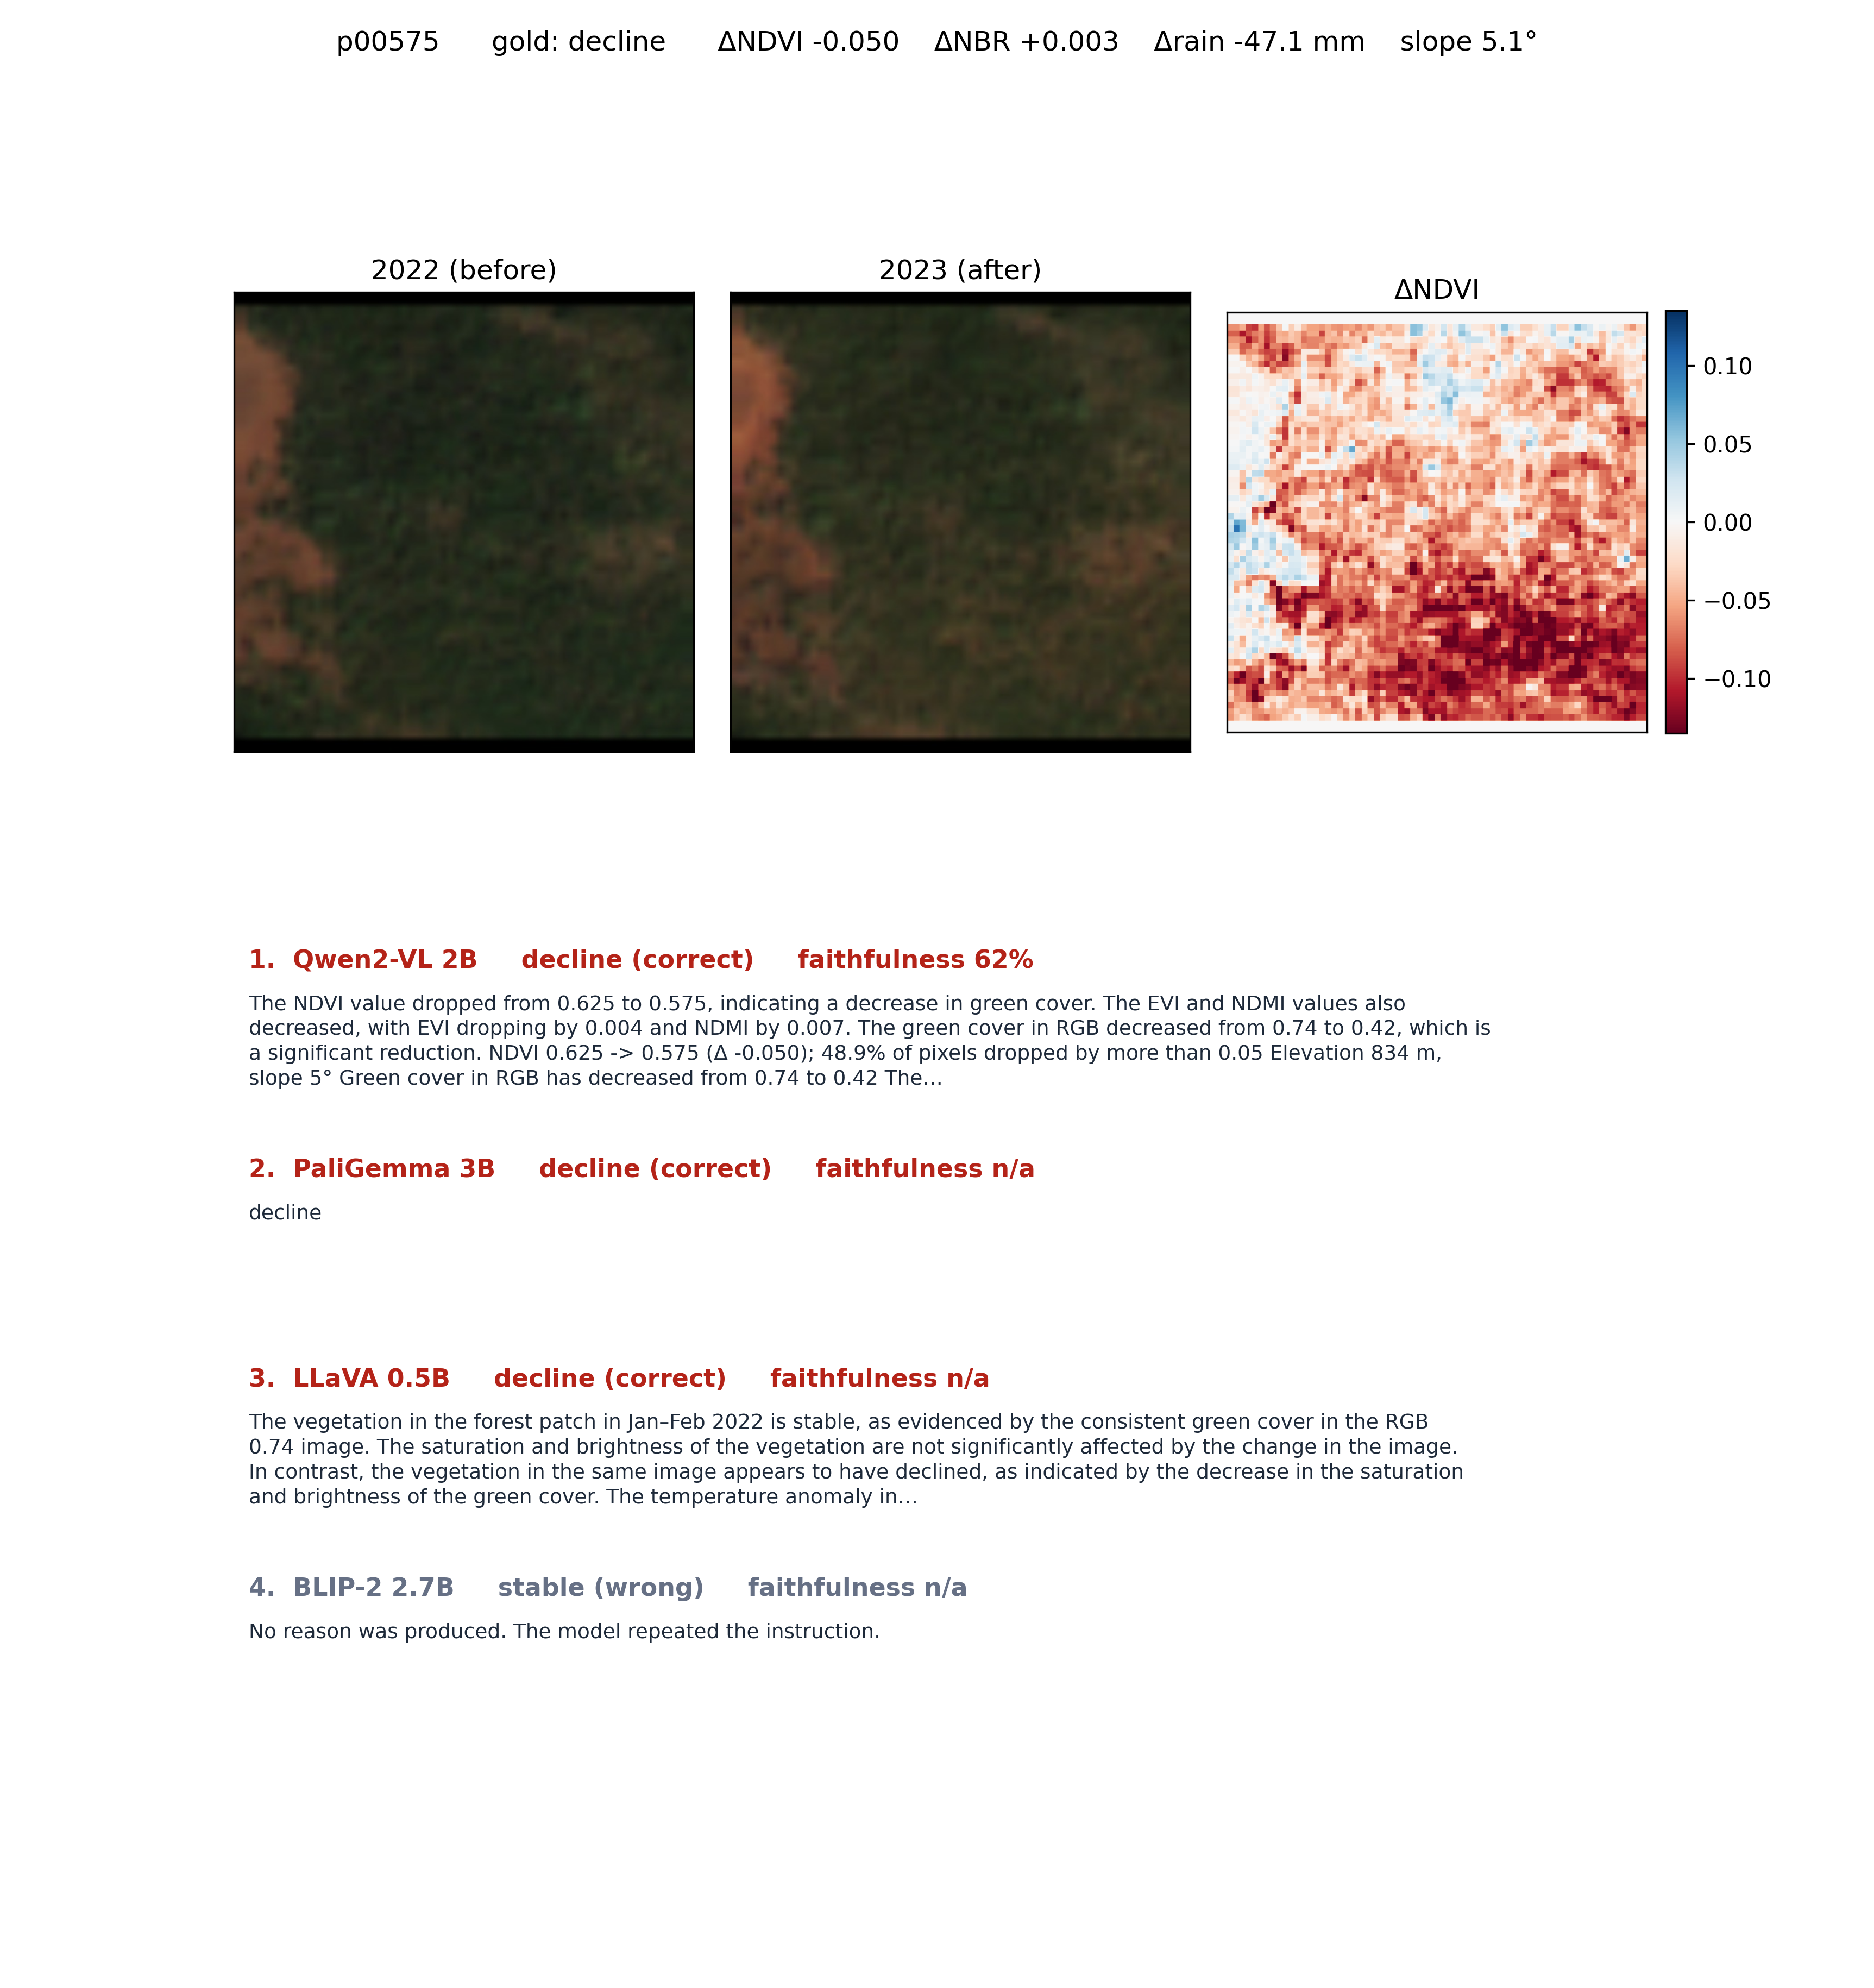
\includegraphics[width=0.74\textwidth]{figures/fig_panel_p00575.png}
\caption{Phase~B explanations for p00575 (gold \texttt{decline}, \dndvi{} $-0.050$), from \file{scripts/make_explanation_report.py}. Three models gave the right class; only Qwen gave a reason grounded in the numbers. The ``faithfulness'' heading in the panel is the project's name for claim correctness.}
\label{fig:panel}
\end{figure}

\section{Phase C: the structured cite-only prompt}
\label{sec:structured}

\subsection{Why it was added}

The free-form prompt gave models room to describe, interpret and speculate, and they used it badly: loops (LLaVA), invented climate causes (Qwen), echoed instructions (BLIP-2). The structured prompt removes that room. It asks the model to copy verified facts, apply a stated rule, and write one sentence about NDVI.

\subsection{What the model receives}

\begin{wherecode}
\file{src/vlm_evidence.py}: \texttt{evidence\_bullets}, \texttt{ndvi\_class\_hint}, \texttt{compact\_evidence\_structured}. \file{src/vlm_eval.py}: \texttt{EXPLAIN\_JSON\_ASK\_STRUCTURED}. \file{scripts/run_explain.py --prompt-style structured} writes \file{results/explain/explain_structured_<model>.json}.
\end{wherecode}

Under the compact table come two new blocks:
\begin{enumerate}
  \item \textbf{\texttt{ALLOWED\_FACTS}}: up to six numbered sentences built from the record, for example ``Patch mean NDVI was 0.625 in 2022 and 0.575 in 2023 ($\Delta$ $-0.050$).'', plus the EVI and NDMI changes, the rainfall totals, the temperature anomalies and the VV change. No class names.
  \item \textbf{\texttt{CLASS\_RULE}}: one line computed from that patch's NDVI change with $\pm0.02$ cut-offs, for example ``NDVI $\Delta \le -0.02 \rightarrow$ decline.'' It is not the \texttt{candidate\_class} field, but it does state a class for the patch.
\end{enumerate}

\begin{tcolorbox}[colback=gray!4,colframe=gray!50,fontupper=\scriptsize]
Images: 2022 (left/first) vs 2023 (right/second). Follow steps in order.\\
Step 1 --- Copy exactly 3 strings from ALLOWED\_FACTS (verbatim) into supporting\_evidence.\\
Step 2 --- Set change\_class using CLASS\_RULE and NDVI $\Delta$ only (stable, decline, or increase).\\
Step 3 --- Write justification as ONE sentence that mentions NDVI only; do not mention rainfall, temperature, or soil unless those lines were copied in Step 1.\\
Set conflicting\_evidence to [] and possible\_driver to "" (empty). Do not state causes or climate drivers.\\
Reply with JSON only: \{"visual\_change": "one short phrase", "change\_class": "stable|decline|increase", "justification": "...", "supporting\_evidence": ["...", "...", "..."], "conflicting\_evidence": [], "possible\_driver": "", "confidence": 0.5\}
\end{tcolorbox}

Only Qwen and LLaVA were run on all 55 test patches, on the MacBook Air's Apple GPU (\texttt{mps}) on 6 October: Qwen in 1,009\,s (18.3\,s per patch), LLaVA in 414\,s (7.5\,s per patch), up to 256 new tokens, greedy decoding.

\subsection{Results}

\begin{table}[H]
\centering
\caption{Phase~C on the 55 test patches (\file{results/explain/explanation_scores.csv}, 6 October; detailed counts recomputed from \file{explain_structured_*.json}).}
\label{tab:phaseC}
\small
\begin{tabular}{lrr}
\toprule
 & Qwen2-VL-2B & LLaVA-Interleave-0.5B \\
\midrule
Class accuracy (explanation mode) & 63.6\,\% (35/55) & 45.1\,\% (23 of 51 answered) \\
Class agrees with \texttt{CLASS\_RULE} & 53/55 & 42/55 \\
Output was complete JSON & 13/55 & 10/55 \\
\texttt{change\_class} left as the template text & 22/55 & 27/55 \\
Checkable claims per explanation & 2.85 & 2.33 \\
Correct claims & \textbf{75.8\,\%} (119/157) & \textbf{71.1\,\%} (91/128) \\
Explanations with $\ge 1$ claim flagged wrong & 36.4\,\% & 34.5\,\% \\
\quad of the flagged claims: change below the dead-band & 35 of 38 & 35 of 37 \\
\quad understatements / sign contradictions & 2 / 1 & 0 / 2 \\
Self-consistency & 100\,\% & 90.7\,\% \\
ROUGE-L against the evidence table & 0.566 & 0.250 \\
Distinct-2 / near-duplicate share & 0.21 / 9.1\,\% & 0.20 / 34.5\,\% \\
\bottomrule
\end{tabular}
\end{table}

\subsection{How to read them}

\paragraph{Claim correctness improved.} Qwen's correct claims rose from 43.8\,\% (3 patches) to 75.8\,\% (55 patches), LLaVA's from 56.7\,\% to 71.1\,\% (both on 55). LLaVA's self-consistency rose from 10\,\% to 91\,\%: its claims now point the same way as its class.

\paragraph{Most remaining ``errors'' are about tiny changes.} Of Qwen's 38 flagged claims, 35 describe a copied change smaller than the scorer's dead-band as a decrease or increase (for example ``EVI $\Delta$ $-0.006$'' or ``green cover 1.00 $\rightarrow$ 0.99''). These numbers are true; the scorer counts any change below 0.02 (0.05 for green cover) as stable. Only 1 Qwen claim and 2 LLaVA claims state the wrong sign. So the 36.4\,\% and 34.5\,\% of explanations ``with a wrong claim'' mostly reflect the strictness of the scorer, not invented facts.

\paragraph{The class comes from the stated rule.} Qwen's class matched \texttt{CLASS\_RULE} on 53 of 55 patches, and in 22 outputs the \texttt{change\_class} field was left as the template text, so the parser took the class from the copied rule. The rule alone scores 63.6\,\% against the labels, exactly Qwen's accuracy in this mode (Figure~\ref{fig:confusionA}f). This is instruction-following, not a new ability to classify.

\paragraph{Explanations became restatements.} ROUGE-L against the evidence table is 0.566 for Qwen, and many outputs repeat one fact: for p00701 all three ``supporting evidence'' items are ``NDVI 0.581 $\rightarrow$ 0.585 ($\Delta$ +0.004)''. LLaVA sometimes invents numbers in the allowed format: for p04508 it wrote ``NDVI $\Delta$ was +0.002'' when the change was $-0.005$. The direction check cannot catch this, because both values fall inside the ``stable'' dead-band.

\paragraph{Formatting.} Only 13 (Qwen) and 10 (LLaVA) outputs were complete JSON; the rest ran past the 256-token limit, mostly because the models copied the whole table. The parser still recovered a class for all Qwen outputs and 51 LLaVA outputs.

\begin{watchout}
\file{results/explain/explanation_scores.json} also contains ``structured'' rows for PaliGemma and BLIP-2 with 40\,\% accuracy. They come from a 5-patch test run on Ada (\texttt{n\_eval = 5}, zero checkable claims), and their source files are not on your laptop. Do not report them.
\end{watchout}

\section{Phase D: the explanation LoRA}
\label{sec:explora}

\subsection{The idea}

If a model sometimes writes good justifications, keep only the good ones and fine-tune the model on them, so that it writes good ones more often. This is a simple form of \emph{distillation}: a ``teacher'' model produces training targets for a ``student''. Here teacher and student are the same model, Qwen2-VL-2B (``2B-on-2B''), because the planned 7B teacher could not be downloaded: job 24225 failed in the download tool and job 24237 hit the disk quota of the Ada home directory.

\subsection{Step 1: building the targets (Ada job 24298)}

\begin{wherecode}
\file{scripts/build_explain_targets.py} and \file{scripts/ada_slurm_explain_targets.sh}. Output: \file{data/explain_targets/train_targets.jsonl} and \file{results/explain/target_filter_report.json}; log \file{results/slurm-explain-targets-24298.log}.
\end{wherecode}

For each of the 256 training patches, the teacher received the label-free compact table and the free-form JSON prompt of Phase~B (up to 256 new tokens). A justification was kept only if (i) its class equalled the label, (ii) it contained at least two checkable claims, and (iii) \emph{all} its claims agreed with the measured changes. \textbf{28 of 256} passed.

\begin{newinfo}
Looking inside \file{train_targets.jsonl} (recomputed for this guide):
\begin{itemize}
  \item The 28 kept targets are \textbf{26 decline, 2 increase and 0 stable}. A filter that requires the class to be right keeps the cases the teacher already handled, and the 2B teacher was mostly right about declines.
  \item In \textbf{12 of the 28}, the \texttt{justification} field holds the teacher's raw output, starting with a code fence (\verb|```json|) and cut off mid-sentence, because the parser could not read the truncated JSON and fell back to the raw text. The student was trained to reproduce these nested, unfinished outputs.
\end{itemize}
\end{newinfo}

\subsection{Step 2: training (Ada job 24389)}

\texttt{python scripts/run\_finetune\_qwen.py --train --eval --target explain --max-train 128 --epochs 1}, with the same LoRA settings as Track~B and the label-free table as input. Because \texttt{--max-train 128} keeps the first 128 training patches by ID, only \textbf{16 of the 28 targets} were used (the log prints ``explain targets kept 16 / 128''). Those 16 are \textbf{all labelled decline}, and 9 of them are the raw, cut-off kind. The single epoch was kept by development accuracy measured in one-word \texttt{evidence\_only} mode (34.5\,\%, the majority level), so the selection step chose nothing in practice.

\subsection{Step 3: testing}

The adapter was tested on the 55 test patches in explanation mode, with the label-free table and the free-form JSON prompt (935\,s). Results (\file{results/explain/explain_qwen_vl_finetuned_ecoexplain.json}, \file{explanation_scores.json}):

\begin{table}[H]
\centering
\caption{Phase~D on the 55 test patches. Interval, macro-F1, confusion and rule agreement recomputed for this guide.}
\label{tab:phaseD}
\small
\begin{tabular}{L{6.0cm}L{8.2cm}}
\toprule
Targets kept by the filter / used in training & 28 of 256 / 16 (all decline) \\
Class accuracy (explanation mode) & \textbf{61.8\,\%} (34/55; 95\,\% interval 48.6--73.5\,\%) \\
Macro-F1 & 0.525 \\
Per class & decline 17/18, stable 0/18 (all called decline), increase 17/19 \\
Answers that match the $\pm0.02$ NDVI rule & 28/55 \\
Checkable claims per explanation & 6.84 \\
Correct claims & 50.5\,\% \\
Explanations with $\ge 1$ wrong claim & 74.5\,\% \\
Self-consistency & 96.4\,\% \\
ROUGE-L against the evidence table & 0.205 \\
\bottomrule
\end{tabular}
\end{table}

\subsection{How to read it}

\begin{itemize}
  \item \textbf{It is not a better explainer.} Claim correctness (50.5\,\%) is lower than structured zero-shot Qwen (75.8\,\%), and three explanations in four contain at least one wrong claim. The student writes many more claims (6.84 per explanation, because its targets included long evidence lists), and more of them are wrong.
  \item \textbf{Its class answers are not comparable with Track~A.} 61.8\,\% comes from a JSON explanation written from the label-free table, after training on 16 justifications; Track~A scores one-word answers. Like the first class LoRA, it calls every stable patch ``decline'' (Figure~\ref{fig:loraclasses}d), and with 16 decline-only targets it could hardly learn otherwise.
  \item \textbf{But it does separate decline from increase.} It was right on 17 of 18 decline and 17 of 19 increase patches, without the label line and without a stated rule. Against always answering ``increase'' that is significant (McNemar: 17 gained, 2 lost, $p < 0.001$), the only label-free classification in the project that is. Two cautions: it never answers ``stable'', and zero-shot Qwen was run in this free-form explanation mode on only 3 patches, so you cannot tell whether the LoRA or the prompt (which asks the model to cite the numbers) produced it. Running zero-shot Qwen in the same mode on all 55 patches would settle it.
  \item \textbf{What it shows.} The pipeline for teacher filtering and explanation fine-tuning works end to end, and a 2B teacher is too weak to produce useful targets: it passed only 28 of 256, almost all of one class. That is a useful pilot result with a clear next step (a stronger teacher, balanced targets, clean JSON).
\end{itemize}

\begin{watchout}
Do not put 61.8\,\% in the same table as 56.4\,\% and 67.3\,\%. Those are one-word classifications with the full card; 61.8\,\% is the class parsed from a JSON explanation written from a label-free table after training on 16 justifications.
\end{watchout}

\section{All explanation phases together}

\begin{figure}[H]
\centering
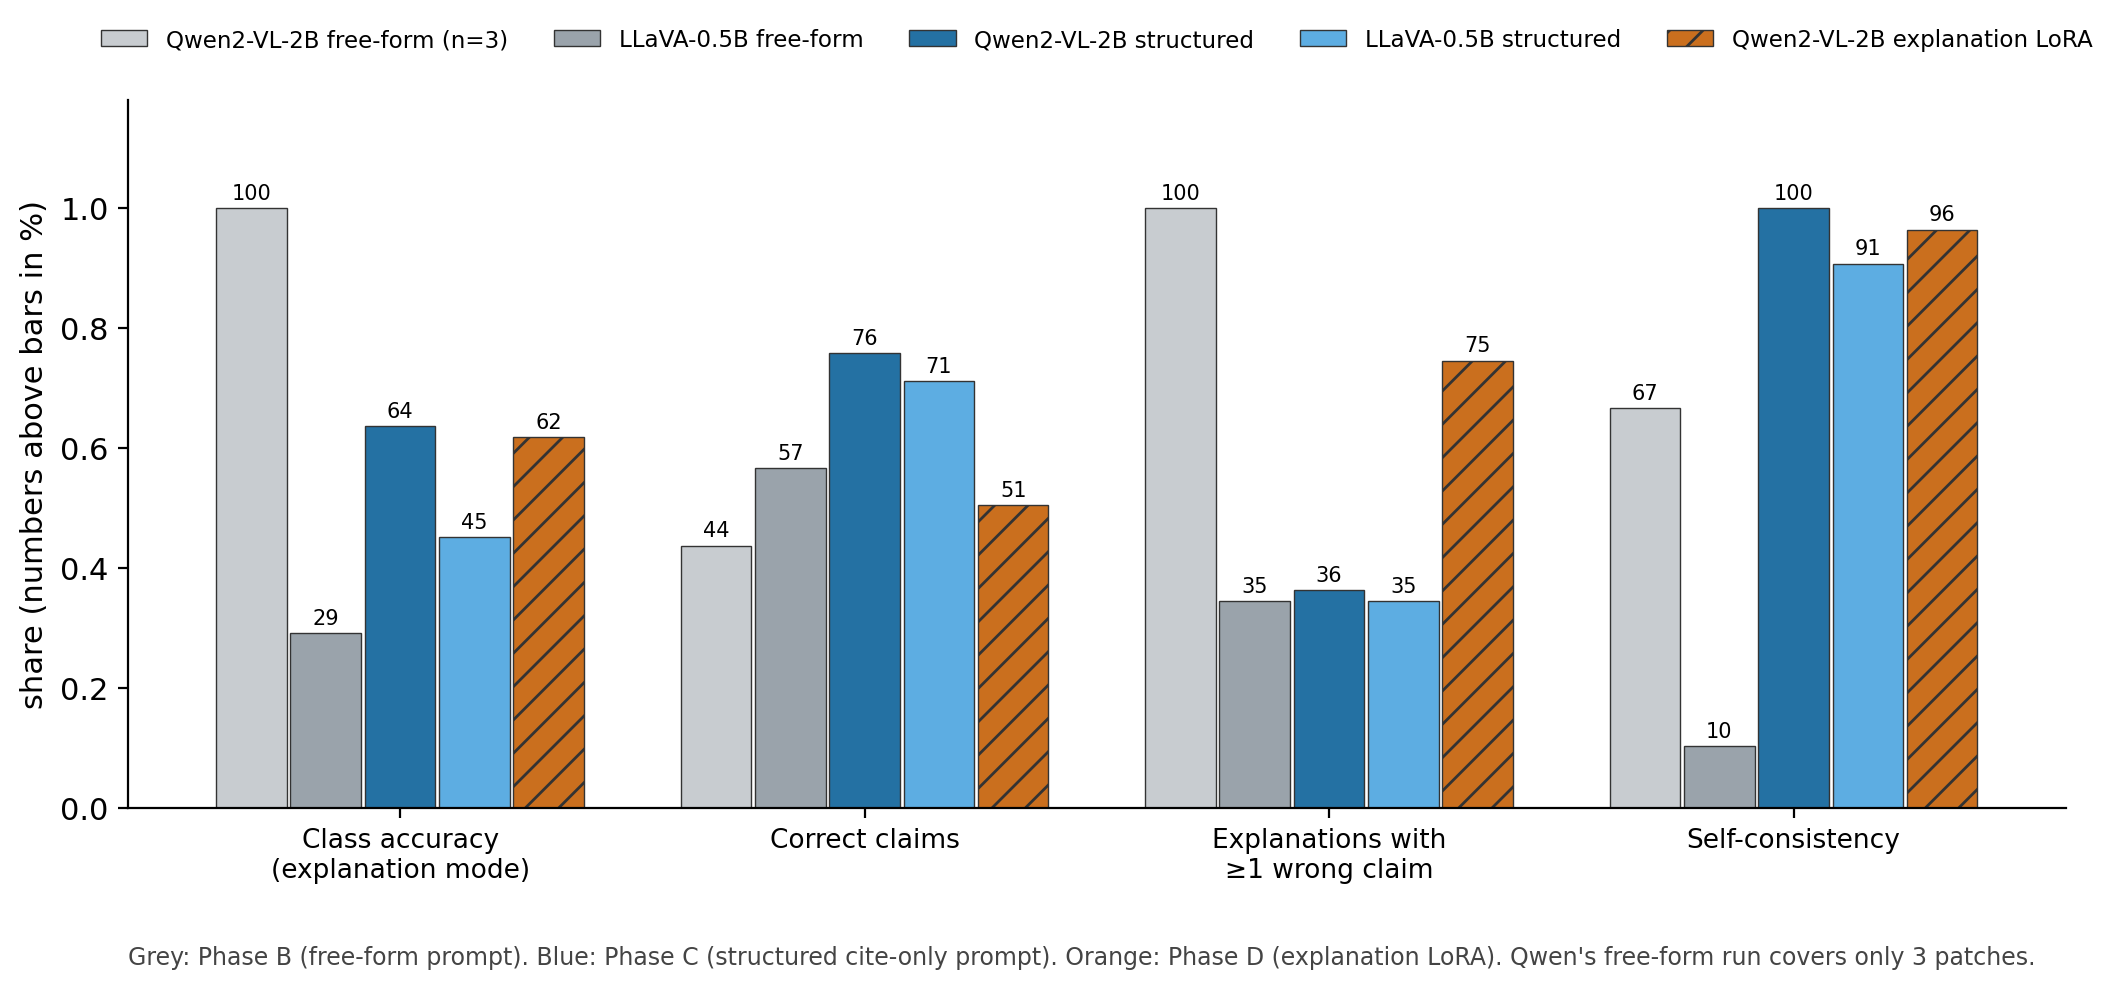
\includegraphics[width=\textwidth]{figures/fig_explain_phases.png}
\caption{Explanation scores across the three phases. Grey: free-form prompt (Qwen on 3 patches only). Blue: structured cite-only prompt. Orange: explanation LoRA. Phase~B values from \texttt{score\_explanations.py --include-legacy}; Phase~C from \file{explanation_scores.csv}; Phase~D from \file{explanation_scores.json}. Made by \file{study_guide_v2/make_figures_v2.py}.}
\label{fig:explphases}
\end{figure}

\begin{plainwords}
The pattern is clear. Free text from small models is unreliable. Telling them exactly which facts they may use makes their claims mostly correct, but then they mostly repeat those facts and follow the stated rule. Fine-tuning on a handful of self-made justifications did not help: it produced longer explanations with more wrong claims.
\end{plainwords}

\begin{newinfo}
\textbf{Which file holds which number.} \file{results/explain/explanation_scores.csv} (6 October) holds the Phase~B rows that were kept and the Phase~C rows (Qwen and LLaVA structured). \file{results/explain/explanation_scores.json} was overwritten on 17 October by the Ada run and now holds Phase~D (plus the two 5-patch rows above). The Phase~B values for Qwen and LLaVA come from \texttt{scripts/score\_explanations.py --include-legacy}. If you re-run the scorer, both files will change: copy them first.
\end{newinfo}

\begin{foryourreport}
In ``Explanation Quality'' (about 900 words):
\begin{itemize}
  \item What the models received (label-free table; \file{check_no_leak.py}) and the two prompts, briefly (prompts in an appendix).
  \item Phase~B in a few sentences per model, with one short example (p00086 or p00575).
  \item Phase~C: Table~\ref{tab:phaseC} (shortened); the dead-band finding; the class follows the stated rule (53/55, ceiling 63.6\,\%); the restatement trade-off.
  \item Phase~D: the 28/256 filter, the 16 decline-only targets, the results, and why it is a pilot.
  \item Figure~\ref{fig:explphases} as the summary.
  \item One sentence on what the scorer measures (evidence consistency) and its limits \citep{jacovi2020,turpin2023}.
\end{itemize}
\end{foryourreport}

\begin{selfcheck}
\begin{enumerate}
  \item What did the models receive in explanation mode instead of the full card, and why?
  \item Describe one failure of each model under the free-form prompt.
  \item What are \texttt{ALLOWED\_FACTS} and \texttt{CLASS\_RULE}?
  \item Why are most of the ``wrong'' claims in Phase~C not really wrong?
  \item Why is Qwen's 63.6\,\% in Phase~C not evidence of better classification?
  \item Give three reasons why the explanation LoRA did not produce better explanations.
  \item Why must 61.8\,\% not be compared with 56.4\,\%?
\end{enumerate}
\end{selfcheck}


\part{Putting it together}
\chapter{What the project shows}
\label{ch:meaning}

\section{The answer to the research question}

\emph{Can vision--language models correctly classify forest vegetation change and generate explanations that are supported by multimodal remote-sensing and climate evidence?}

\paragraph{Classification: no, not from the evidence.} With the full evidence card, Qwen2-VL-2B reached 56.4\,\% zero-shot and the other three models stayed at the level of guessing one class. But the card's last line states the trend and the label, and without it Qwen falls to 32.7\,\% (it answers ``stable'' for every patch; $p = 0.011$). With the same label-free table for every model, LLaVA reaches 43.6\,\%, not significantly above the 34.5\,\% baseline, and a balanced, label-free LoRA of Qwen on 16 patches reaches 36.4\,\%. A one-number threshold on the card's \dndvi{} reaches 94.5\,\%: the information is there, and small general-purpose VLMs do not extract it. The one hopeful sign is in explanation mode, where the explanation LoRA separates decline from increase (61.8\,\%, significant against the baseline) without the label line, though it never answers ``stable'' and its zero-shot counterpart is untested.

\paragraph{Explanations: only when tightly constrained.} Free-form explanations were missing, repetitive, or in conflict with the numbers. A structured cite-only prompt made 71--76\,\% of checkable claims agree with the measurements, with very few sign errors, but the explanations then mostly restate the supplied facts and the class follows the stated rule. A pilot explanation LoRA trained on 16 self-generated justifications did not improve on that (50.5\,\% correct claims).

\begin{plainwords}
In one line: \emph{small open VLMs can be made to repeat the evidence correctly, but they do not yet interpret it.} That is a useful, honest finding, and the benchmark makes it measurable.
\end{plainwords}

\section{The five pre-registered hypotheses}

``Pre-registered'' means written down before seeing results (roadmap Section~9), so they cannot be adjusted afterwards.

\begin{longtable}{L{0.8cm}L{4.4cm}L{2.3cm}L{6.6cm}}
\caption{Status of the roadmap's hypotheses.}\label{tab:hyp}\\
\toprule
 & \textbf{Hypothesis} & \textbf{Status} & \textbf{Evidence} \\
\midrule
\endfirsthead
\toprule
 & \textbf{Hypothesis} & \textbf{Status} & \textbf{Evidence} \\
\midrule
\endhead
H1 & Combined images and numbers beat images alone & Not tested & No model was run zero-shot with images only on the same patches. \\
H2 & Combined input covers more evidence but adds unsupported causal claims & Not tested & Needs an images-only versus combined comparison of explanations. \\
H3 & Models differ in classification, groundedness and calibration & Partly supported & Classification: with the full card Qwen 56.4\,\% versus 32.7--36.4\,\% (unequal inputs); with equal label-free inputs LLaVA 43.6\,\% versus Qwen 32.7\,\%, not significant ($p = 0.44$). Groundedness: 75.8\,\% versus 71.1\,\% correct claims (structured). Calibration not measured. \\
H4 & Confidence tracks correctness, but models are overconfident & Not tested & No usable confidence values. \\
H5 & Structured explanations contain fewer contradictions than free ones & Partly supported & Claim correctness and self-consistency rose for both models; true sign contradictions became rare (1 and 2); the share of explanations with a flagged claim stayed about the same, mostly because of the dead-band. \\
\bottomrule
\end{longtable}

\begin{foryourreport}
Hypotheses that were not tested are not failures; they are future work. Say so plainly: ``H1, H2 and H4 were not tested because the images-only condition and confidence elicitation were not run.''
\end{foryourreport}

\section{Were the objectives achieved?}

The objectives come from the roadmap and the handbook (the first guide reconstructed twelve of them). For an Independent Study, three labels are fair: \textbf{achieved}, \textbf{achieved within pilot scope} (the core aim met, the full roadmap depth left for later) and \textbf{extension} (deliberately left for future research).

\begin{longtable}{L{4.2cm}L{2.0cm}L{8.0cm}}
\caption{Objectives and their status.}\label{tab:objectives}\\
\toprule
\textbf{Objective} & \textbf{Status} & \textbf{Evidence} \\
\midrule
\endfirsthead
\toprule
\textbf{Objective} & \textbf{Status} & \textbf{Evidence} \\
\midrule
\endhead
O1 Matched-season multi-source benchmark & Achieved & 366 patches, five sources, 15 GeoTIFFs each, matched windows, median composites, checks passed. \\
O2 Defensible reference labels & Pilot scope & Percentile rule for all 366; 19 human checks (8 agree); no second annotator or audit. \\
O3 Prevent leakage & Pilot scope & Coordinates removed; summary line stated and measured (label-free reruns); \texttt{evidence\_only} and \texttt{compact} modes, \file{check_no_leak.py}; training refuses the full card; spatial block split written but not yet evaluated. \\
O4 Standard evidence cards & Pilot scope & Rule-based cards from the rasters; compact and structured variants; no false-colour images; boxes on 3 patches. \\
O5 Controlled model comparison & Pilot scope & Four open models on identical test patches; an equal-input \texttt{compact} run for Qwen and LLaVA (PaliGemma gated, BLIP-2 unparsable); no images-only condition; no proprietary model. \\
O6 Proper classification metrics & Pilot scope & Accuracy in the repository; macro-F1, Wilson intervals, McNemar tests and confusion matrices in this guide. \\
O7 Explanation evaluation & Pilot scope & Automatic claim checking, self-consistency, copying and diversity scores; no human rating. \\
O8 Confidence and consistency & Extension & No calibration or repeated runs. \\
O9 Statistical analysis & Extension & Wilson and McNemar only; no bootstrap or mixed models. \\
O10 Reproducible release & Achieved & Repository with dataset, splits, code, notebooks, results and Slurm logs. \\
O11 Fine-tune an open model (added in September) & Achieved & Balanced, label-free class LoRA 36.4\,\% (16 patches; the earlier full-card 67.3\,\% superseded); explanation LoRA pilot 61.8\,\% (16 targets). \\
O12 Justifications from models (added in October) & Achieved & Explanation mode, parser, scorer, visual report; structured protocol on all 55 test patches. \\
\bottomrule
\end{longtable}

\section{Limitations}
\label{sec:limits}

These limitations define where your claims stop. They do not mean the study is incomplete.

\begin{enumerate}
  \item \textbf{Labels.} Automatic, relative (percentile) labels with slightly overlapping class ranges; 19 human checks with 42\,\% agreement; no second annotator. Accuracy means agreement with a rule.
  \item \textbf{One place, one pair of years, one season.} No claim generalises to other forests or years.
  \item \textbf{Subtle change and the weather.} Most changes are below 0.05 NDVI, and 2023 was unusually dry and warm everywhere; some ``decline'' may be early seasonal drying.
  \item \textbf{Random split.} Training and test patches can touch; spatial autocorrelation can inflate fine-tuned results \citep{roberts2017,ploton2020}. A spatial block split now exists (\file{data/splits_spatial/}) but has not been evaluated.
  \item \textbf{Small test set.} 55 patches give 95\,\% intervals about $\pm13$ points wide.
  \item \textbf{Small models in reduced settings.} 0.5--3B checkpoints, images shrunk to 336 pixels on the laptop, 48-token answers.
  \item \textbf{Unequal inputs.} In the full-card run PaliGemma received one NDVI line and BLIP-2 no card at all. The \texttt{compact} rerun equalised the input, but PaliGemma could not be loaded and BLIP-2 gave no parsable answer, so only Qwen and LLaVA have equal-input scores.
  \item \textbf{The summary line.} The full card states the trend word and \texttt{candidate\_class}; the full-card accuracies reflect use of that line. Without it no one-word classifier beats the baseline. Qwen's \texttt{evidence\_only} answers were overwritten, so only its score (32.7\,\%) survives for that mode.
  \item \textbf{Tiny fine-tunes.} Every reported LoRA used 16 examples for one epoch. The class LoRA is now balanced (6/5/5); the explanation LoRA's 16 targets are all decline (9 of them malformed).
  \item \textbf{Structured explanations.} Run for Qwen and LLaVA only; the class follows the stated rule; many outputs exceed the token limit; justifications restate supplied facts.
  \item \textbf{Padding bias} in every number on the card (about 8\,\% low; edge patches much more).
  \item \textbf{Parsing.} The original results counted echoed prompts as answers (BLIP-2). The parser was fixed on 20 October; the old result files were not re-parsed.
  \item \textbf{Explanation metric.} Pattern-based, blind to negation; its dead-band flags true small changes and misses invented numbers inside the dead-band. It measures evidence consistency, not faithfulness \citep{jacovi2020}.
  \item \textbf{No calibration, repeated runs or human rating} of explanations.
  \item \textbf{Coarse climate data}, the same for all classes, so it cannot explain patch-level change.
  \item \textbf{Image input.} Dark true-colour chips only; the much more informative \dndvi{} maps and false-colour images were never shown to the models.
  \item \textbf{Test-set adaptivity.} Prompts were changed and the closed-set probe designed after seeing test results.
\end{enumerate}

\section{Future research}
\label{sec:future}

Write this as a research programme, not as a list of apologies.

\begin{description}[style=nextline]
  \item[Label validation] Several expert annotators, inter-rater agreement (Cohen's $\kappa$; \citealp{cohen1960}), and explicit handling of borderline patches.
  \item[Label-free evaluation as the default] Done for Qwen and LLaVA (Phase~E). Still to do: PaliGemma (needs a Hugging Face token on the laptop) and a BLIP-2 setting that yields answers; keep each run's per-model file separately.
  \item[Explanation mode without fine-tuning] Run zero-shot Qwen with the free-form explanation prompt on all 55 patches, to see whether the explanation LoRA's decline/increase separation comes from the prompt or the training.
  \item[Spatial validation] A spatial block split as a second test set \citep{roberts2017,ploton2020}.
  \item[Which input helps?] The roadmap's images-only and numbers-only conditions alongside the combined one (H1, H2), with every model given the same text.
  \item[Proper fine-tuning] 48 (16 per class) or all 256 training patches, balanced, without the summary line, with early stopping on the development set; the 16-patch balanced run is only the first step.
  \item[The spatial test] Evaluate the leak-free protocol on \file{data/splits_spatial/} with its own baseline (38.9\,\%).
  \item[Better explanation targets] A stronger teacher (a 7B model on scratch disk, not the home quota), class-balanced targets, clean JSON, and blind human rating of the outputs.
  \item[Domain-adapted models and inputs] Remote-sensing VLMs such as GeoChat \citep{kuckreja2024}; \dndvi{} maps and false-colour images as inputs.
  \item[Uncertainty] Elicited confidences, Brier score and calibration error \citep{brier1950,guo2017}, repeated decoding.
  \item[Cleaner evidence] Statistics on unpadded chips; a parser that ignores echoed prompts.
  \item[More places and years] Other central-Indian reserves and multi-year stacks to separate drought, phenology and real disturbance; fire and uncertain classes re-enabled.
\end{description}

\begin{selfcheck}
\begin{enumerate}
  \item Answer the research question in two sentences, one per half.
  \item Which hypotheses could not be tested, and why?
  \item Name five limitations that come from the data and five that come from the models or the evaluation.
  \item Which single future step would most change the interpretation of the explanation LoRA's 61.8\,\%, and why?
\end{enumerate}
\end{selfcheck}


\part{From understanding to your report}
\chapter{Your figures and tables: a check of everything you have}
\label{ch:figures}

Figures are often the first thing a professor reads. This chapter checks every figure the project has, says which are correct, which need fixing and which should not be used, and lists the tables the report needs.

\section{Your professor's rules for figures and tables}

\begin{itemize}
  \item Figures and tables appear close to where they are first mentioned.
  \item Related panels are combined into one figure labelled (a), (b), (c).
  \item Text in figures must be legible after scaling (at least about 8\,pt); check by printing one page.
  \item Tables are real tables (\texttt{booktabs} in LaTeX), never screenshots of tables.
  \item The study-area map shows the whole of India, not trimmed at the top.
  \item Extra figures and tables go to an appendix.
\end{itemize}

\section{Every figure, checked}

\begin{longtable}{L{4.0cm}L{4.6cm}L{2.0cm}L{3.4cm}}
\caption{All figures in the project. ``Main'' = main text; ``App.'' = appendix.}\label{tab:figaudit}\\
\toprule
\textbf{File} & \textbf{What it shows} & \textbf{Status} & \textbf{Use} \\
\midrule
\endfirsthead
\toprule
\textbf{File} & \textbf{What it shows} & \textbf{Status} & \textbf{Use} \\
\midrule
\endhead
\file{papers/acl/fig_workflow.png} & your five-stage workflow & needs fixing & Main (Methods), after the fixes in Section~\ref{sec:fixworkflow} \\
\file{study_guide_v2/figures/fig_workflow_corrected.png} & the same figure with the fixes made & correct & Main, if you prefer it to fixing your own \\
\file{results/ecoexplain_vlm_pipeline.png} & an older pipeline drawing & outdated & Do not use: says ``LLaVA-1.5'', ``train on the train split'' and ``64\,$\times$\,64 pixels'' \\
\file{results/result1.png} & notebook flow 01--09 & outdated & Do not use: says ``LLaVA-1.5'' \\
\file{results/result2.png} & zero-shot results as an image of a table & wrong & Do not use: wrong encoder for LLaVA (``CLIP-ViT-L/14'', really SigLIP), and a table as an image \\
\file{results/explain/summary_scores.png} & early explanation-mode accuracy & outdated & Do not use: Qwen bars from 3 patches, before Phases C and D \\
\file{study_guide/figures/fig_patch_map.png} & candidate pool and selected patches by class and split & correct & Main (study area), next to an India map \\
\file{fig_ndvi_labels.png} & \dndvi{} distribution and the percentile rule & correct & Main (labelling) \\
\file{fig_label_vs_trend.png} & label against the card's trend words & correct & Main or App. \\
\file{fig_examples.png} & four test patches, colour pairs and \dndvi{} maps & correct & Main (dataset) \\
\file{fig_climate_by_class.png} & climate by class and year & correct & Main or App. \\
\file{fig_padding_bias.png} & the padding bias & correct & App. or Limitations \\
\file{fig_accuracy_overview.png} & classification runs with intervals & superseded & Use \file{fig_accuracy_v2.png} instead \\
\file{study_guide_v2/figures/fig_accuracy_v2.png} & classification runs up to 17 Oct & superseded & Use \file{fig_accuracy_v3.png} \\
\file{study_guide_v3/figures/fig_accuracy_v3.png} & every classification run, labelled by input, incl.\ the leak-free reruns & correct & Main (Track~A) or App. \\
\file{study_guide_v3/figures/fig_leakfree_confusion.png} & Qwen with and without the summary line; LLaVA with the compact table & correct & Main (Track~A): the key figure \\
\file{fig_confusion.png} & six confusion matrices & correct & Main: panels (a), (b); others App. \\
\file{study_guide_v2/figures/fig_lora_classes.png} & two LoRA runs (up to 17 Oct) & superseded & Use \file{fig_lora_v3.png} \\
\file{study_guide_v3/figures/fig_lora_v3.png} & training mix and test confusion of all three LoRA runs & correct & Main (fine-tuning) \\
\file{fig_explain_structured.png} & free-form against structured (Qwen, LLaVA) & superseded & Use \file{fig_explain_phases.png} \\
\file{study_guide_v2/figures/fig_explain_phases.png} & all explanation phases, four scores & correct & Main (explanations) \\
\file{fig_panel_p00575.png} & one patch, four models' free-form explanations & correct & App. (crop the empty space) \\
\file{fig_otsu_p01289.jpg} & Otsu boxes on one patch & pre-colour-fix & App. only, with a caption note \\
\textbf{study-area map of India} & --- & \textbf{missing} & Main: must be made (Section~\ref{sec:map}) \\
\bottomrule
\end{longtable}

\begin{watchout}
The per-model files in \file{results/protocol/} still label LLaVA ``LLaVA-1.5, CLIP-ViT-L/14''. If you plot from them, take the model name from Table~\ref{tab:models}, not from the file.

Figures saved under \file{study_guide/figures/}, \file{study_guide_v2/figures/} and \file{study_guide_v3/figures/} were made for learning. If you put one in the report, regenerate it (the scripts are \file{study_guide/make_figures.py} and \file{study_guide_v2/make_figures_v2.py}), check every label, and write your own caption. A figure in your report is your responsibility.
\end{watchout}

\section{Fixing your workflow figure}
\label{sec:fixworkflow}

Your figure (Figure~\ref{fig:workflow-yours}) is clear and well designed. Three box texts in stage~05 and two in stage~03 are inaccurate or vague, and two arrows are missing. Table~\ref{tab:workflowfix} lists the changes with the line numbers in \file{papers/acl/make_workflow_figure.py}.

\begin{longtable}{L{1.3cm}L{5.3cm}L{7.6cm}}
\caption{Changes to \file{make_workflow_figure.py}. A corrected copy is \file{study_guide_v2/make_workflow_figure_corrected.py} (every change is marked \texttt{CORRECTED} or \texttt{ADDED}).}\label{tab:workflowfix}\\
\toprule
\textbf{Line} & \textbf{Now} & \textbf{Change to, and why} \\
\midrule
\endfirsthead
\toprule
\textbf{Line} & \textbf{Now} & \textbf{Change to, and why} \\
\midrule
\endhead
219 & Track~A: ``Condition C: T0/T1 RGB + card / Qwen2-VL-2B $\cdot$ PaliGemma-3B / LLaVA-Interleave-0.5B $\cdot$ BLIP-2 / Full card and evidence\_only'' & ``Qwen2-VL-2B, LLaVA-0.5B: T0/T1 + full card / PaliGemma-3B: T0/T1 + NDVI line only / BLIP-2: stitched T0|T1, no card / evidence\_only: label line removed''. \emph{Why:} the four models did not receive the same input (Table~\ref{tab:inputs}). \\
230--231 & Track~B: ``(smoke test)'' and ``100\% run with leak is invalid'' & Title ``(16 patches, 1 epoch)''; body ``full card at train and test / first 16 training patches (9/6/1) / 256-patch runs reached 100\% by reading the label, so they are excluded''. \emph{Why:} the reported run should be described by its size, and the reason for excluding the 100\,\% runs is clearer than the word ``invalid''. \\
242--243 & Track~C: ``Free-form vs structured cite-only / Claims scored against the card / Optional 2B-on-2B explain LoRA'' & ``free-form prompt $\rightarrow$ structured cite-only prompt / claim directions checked against measured $\Delta$ / explanation LoRA pilot: 16 filtered 2B targets, all labelled decline''. \emph{Why:} claims are checked against the \emph{measured changes}, not ``the card''; and the explanation LoRA was run, so it is not ``optional''. \\
209 & ``05 Three evaluation tracks (do not mix the scores)'' & ``05 Three evaluation tracks (inputs differ: do not mix the scores)''. \emph{Why:} says why. \\
165, 176, 187 & stage~03 box texts & RGB chips: ``on a 512\,$\times$\,512 canvas; BLIP-2: one stitched image''. Label: give the cut-offs ``q15 = $-$0.038 $\cdot$ q85 = +0.003''. Card: ``last line repeats candidate\_class=''. \\
after 189 and 206 & arrows only through the middle column & add arrows from Earth Engine to the RGB and card boxes, and from those boxes to the split box: all three feed every record. \\
\bottomrule
\end{longtable}

\begin{figure}[H]
\centering
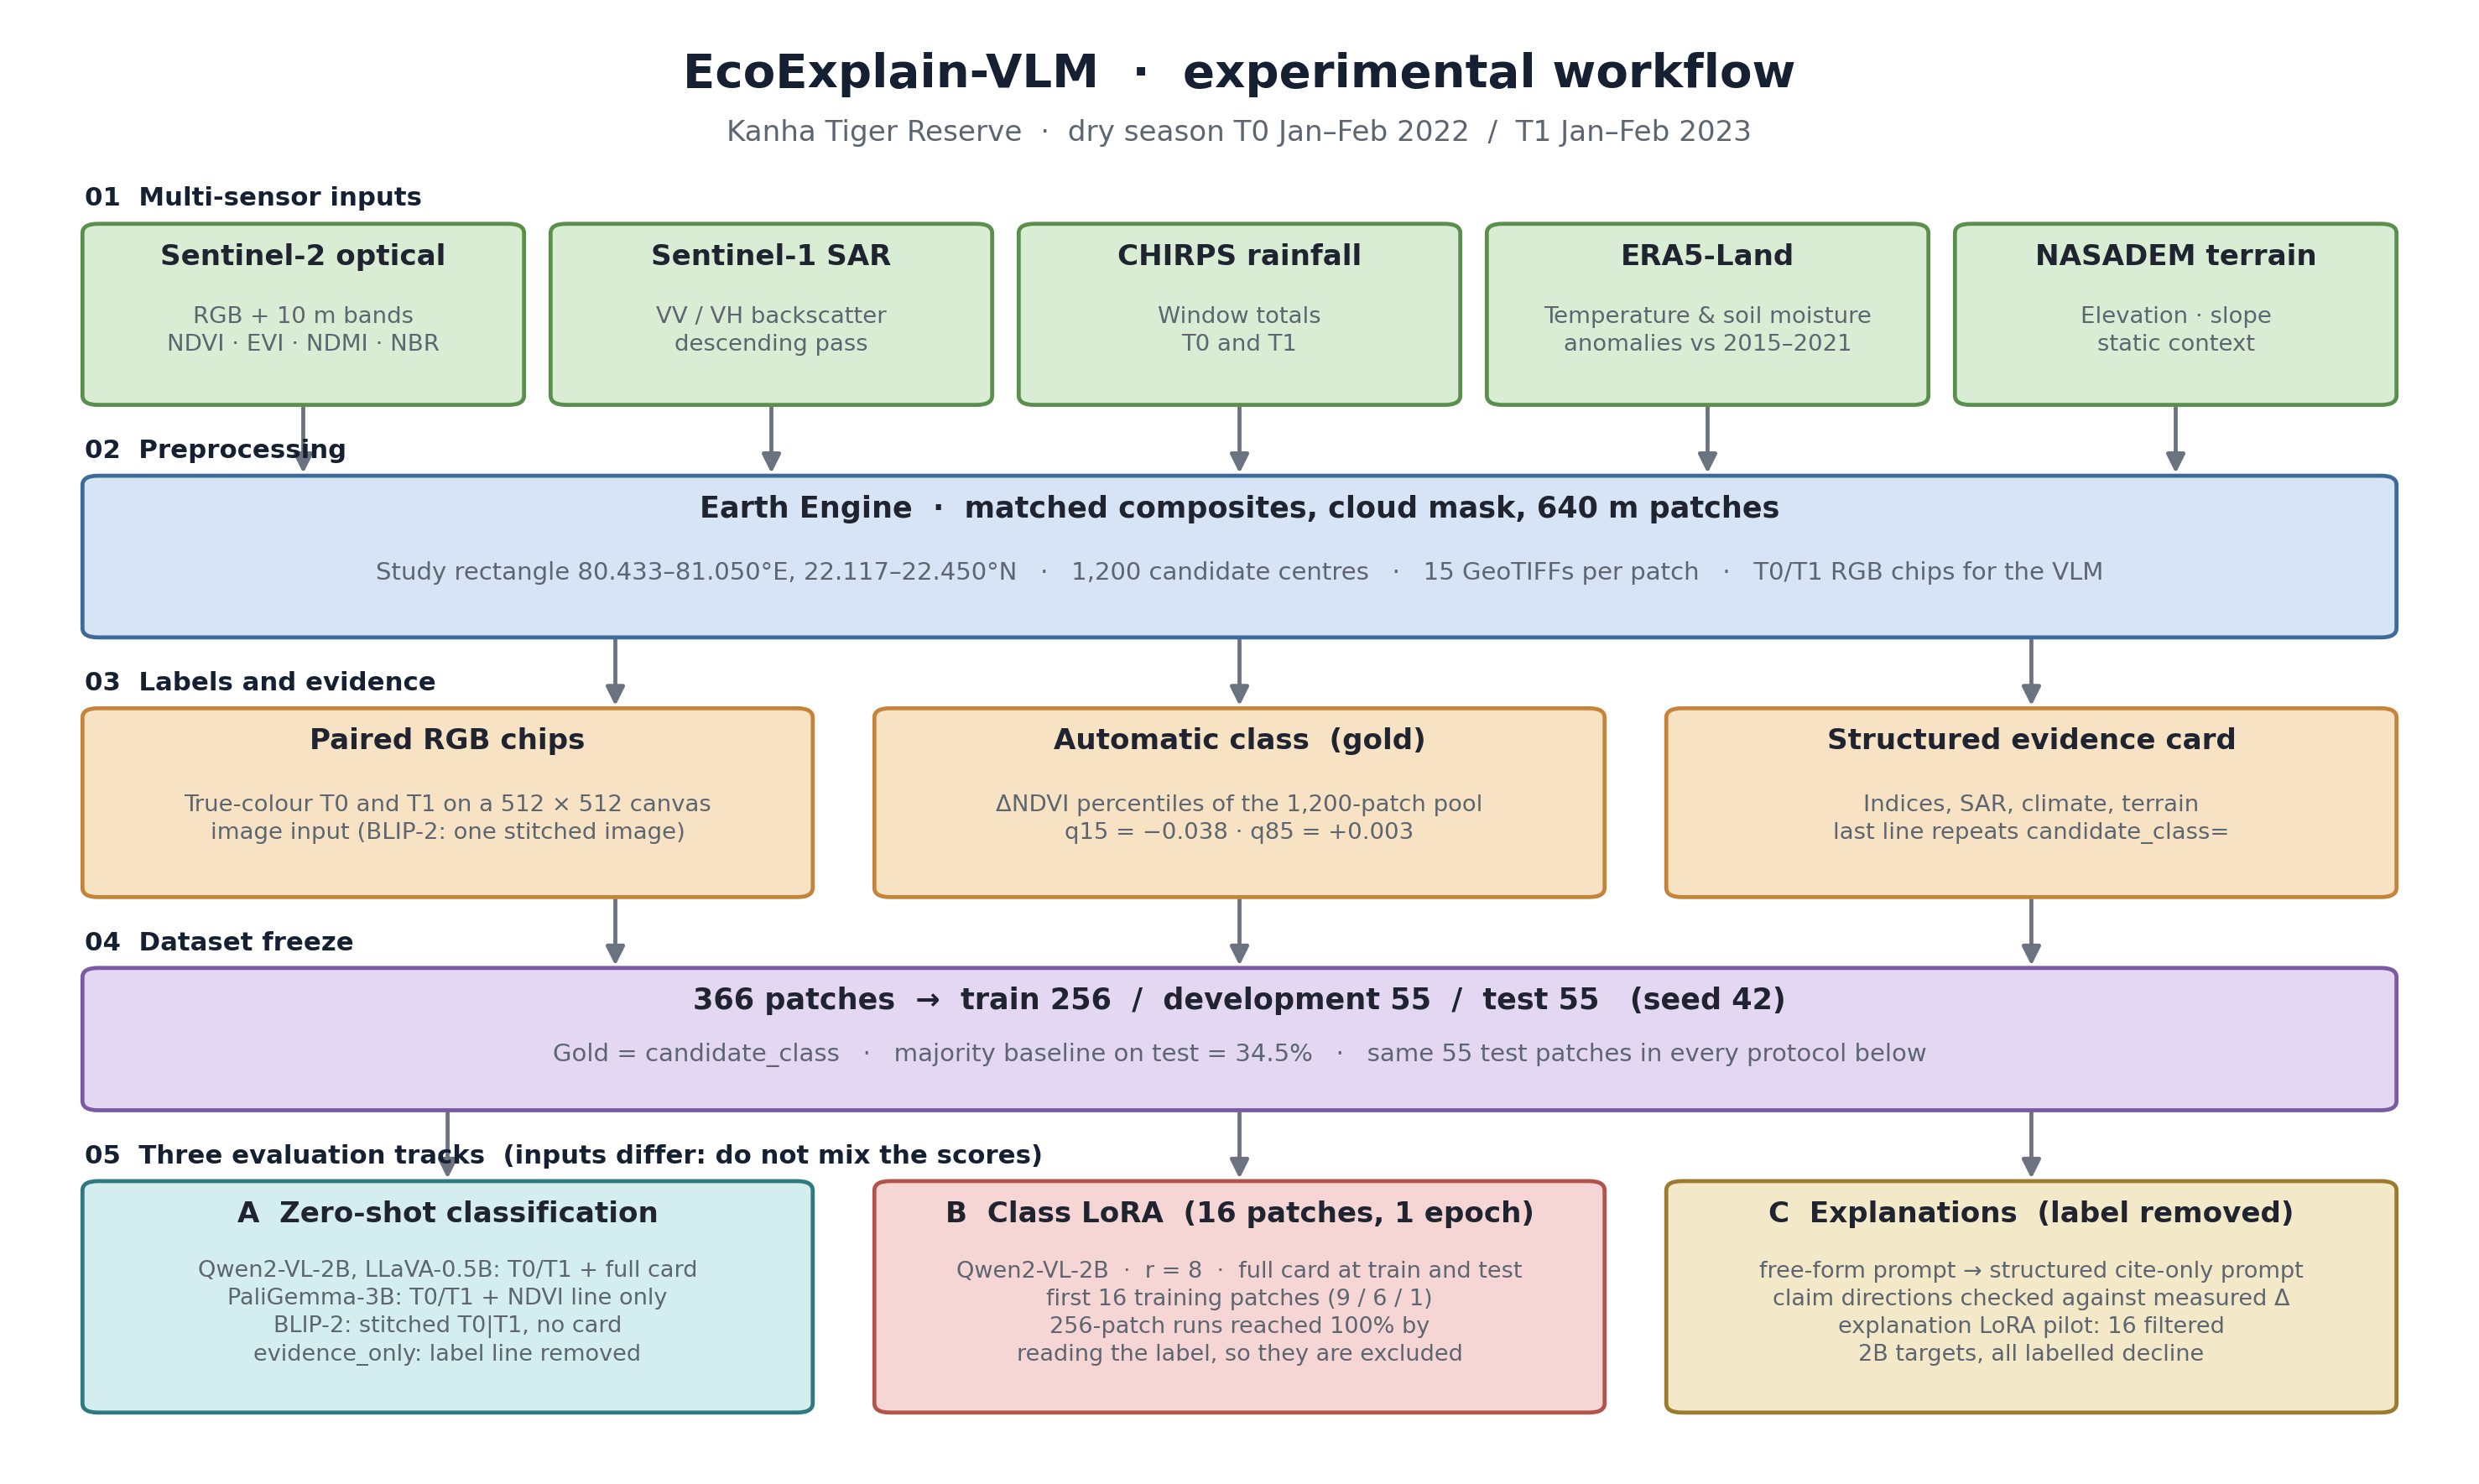
\includegraphics[width=\textwidth]{figures/fig_workflow_corrected.png}
\caption{Your workflow figure with the changes of Table~\ref{tab:workflowfix} (\file{study_guide_v2/make_workflow_figure_corrected.py}). Compare it box by box with Figure~\ref{fig:workflow-yours}.}
\label{fig:workflow-corrected}
\end{figure}

\begin{plainwords}
You can either edit your own script with the changes above (better: it stays your figure) or use the corrected copy. Either way, run it once more after any later change to the text of the report, so that the figure and the text say the same thing.
\end{plainwords}

\section{The study-area map}
\label{sec:map}

Your professor asks for a study-area map showing the whole of India without trimming at the top. You do not have one yet. A good layout has two or three panels:
\begin{enumerate}[label=(\alph*)]
  \item India with state boundaries and Madhya Pradesh highlighted. Use the official Survey of India boundary (from the Survey of India or the Bhuvan portal); maps of India in Indian academic work are expected to follow it, and many global boundary datasets do not.
  \item Madhya Pradesh with the reserve (for example, the boundary from the World Database on Protected Areas) and the study rectangle.
  \item The rectangle with the 366 patch points coloured by class (the content of Figure~\ref{fig:patchmap}).
\end{enumerate}
QGIS is the easiest tool; Python with \texttt{geopandas} and \texttt{matplotlib} also works. Add a north arrow, a scale bar and the coordinate grid.

\section{Tables the report needs}

\begin{table}[H]
\centering
\small
\begin{tabularx}{\textwidth}{lYl}
\toprule
Table & Content & Based on \\
\midrule
Data sources & collection, variables, resolution, scenes & Table~\ref{tab:sources} \\
Dataset summary & patches, classes, split, baseline, human agreement & Table~\ref{tab:split} and Chapter~\ref{ch:stage03} \\
Model inputs & what each model received & Table~\ref{tab:inputs} \\
Classification results & accuracy, interval, macro-F1, input & Table~\ref{tab:trackA}; baselines from Chapter~\ref{ch:trackA} \\
LoRA configuration & settings of both runs & Table~\ref{tab:classlora} \\
Fine-tuning jobs (App.) & all Ada jobs & Table~\ref{tab:ftruns} \\
Explanation results & Phases B, C, D & Tables~\ref{tab:phaseB}--\ref{tab:phaseD} (shortened) \\
\bottomrule
\end{tabularx}
\end{table}

\begin{foryourreport}
Your current draft (ACL two-column format) has one figure. A report of 8,500--10,000 words can carry about six to eight figures in the main text: the study-area map, the workflow, the \dndvi{} labelling figure, the example patches, the classification results, the LoRA confusion matrices, and the explanation summary. In two-column format, use \texttt{figure*} for wide figures (workflow, examples) and \texttt{figure} with \texttt{width=\textbackslash columnwidth} for narrow ones.
\end{foryourreport}

\begin{selfcheck}
\begin{enumerate}
  \item Which existing figures should not appear in the report, and why?
  \item What exactly is wrong with Track~A in your workflow figure?
  \item What must the study-area map show, according to your professor?
\end{enumerate}
\end{selfcheck}

\chapter{Correcting your current draft}
\label{ch:draft}

This chapter reviews your latest draft, section by section. It is the version you pasted on 17 October, saved as \file{report/quillbot_parts/full_paper_v2.tex}. Line numbers refer to that file; if your Overleaf copy has moved on, search for the quoted words instead.

\begin{watchout}
This chapter tells you \emph{what} is wrong and \emph{what is true}. It does not give replacement sentences, because the sentences must be yours. Fix the facts first, then the citations, then the structure, and only then the wording.
\end{watchout}

\section{Since 17 October: what you fixed and what to check now}

Your status note of 20 October reports these as done. I have not seen the updated Overleaf draft, so treat the right-hand column as the check to make, not as confirmation.

\begin{longtable}{L{5.6cm}L{8.6cm}}
\caption{Issues you report as fixed, and how to confirm each one in the draft.}\label{tab:fixed}\\
\toprule
\textbf{Reported fixed} & \textbf{Check in the draft} \\
\midrule
\endfirsthead
\toprule
\textbf{Reported fixed} & \textbf{Check in the draft} \\
\midrule
\endhead
Structure aligned to workflow steps 1--6 and tracks A/B/C & The figure's Track~A box no longer says every model received the card (Chapter~\ref{ch:figures}); the text uses one naming scheme. \\
Keywords match the abstract & Every keyword appears in the abstract or the introduction. \\
Introduction reframed (GeoChat, limitations, LoRA wording) & It cites its sources again (\texttt{\textbackslash citep}), and it is 1,000--1,200 words. \\
Numbers not mixed (56.4 / 67.3 / 61.8 / 75.8 / 71.1) & Each number appears with its input and protocol, and none of them sits in a column with another protocol's numbers. \\
LoRA honesty (9/6/1, 0/18 stable) & Now go one step further: the result to cite is the balanced, leak-free 36.4\,\% (below). \\
\bottomrule
\end{longtable}

\subsection*{New checks required by the 19--20 October reruns}

\begin{enumerate}
  \item \textbf{Primary classification table.} Put the leak-free runs first (Qwen \texttt{evidence\_only} 32.7\,\%, Qwen and LLaVA \texttt{compact} 32.7\,\% and 43.6\,\%), then the full-card runs labelled as such (Chapter~\ref{ch:results}).
  \item \textbf{Track~B number.} Replace 67.3\,\% by 36.4\,\% (balanced 6/5/5, label-free, Ada job 29575, ``stable'' for 53 of 55). Mention 67.3\,\% only as a superseded run.
  \item \textbf{No ``Qwen did not copy the label'' argument.} If the draft uses version~2's observation as evidence for Qwen's skill, remove it: the trend words it followed are in the summary line (Chapter~\ref{ch:trackA}).
  \item \textbf{State the size of the drop}: 56.4\,\% $\rightarrow$ 32.7\,\% without the line ($p = 0.011$).
  \item \textbf{LLaVA's 43.6\,\%} with ``not significantly above the baseline ($p = 0.44$)''.
  \item \textbf{PaliGemma and BLIP-2}: no leak-free result (gated model; 0 of 55 parsable), and BLIP-2's 32.7\,\% is a parsing artefact.
  \item \textbf{Methods} mentions the \texttt{compact} mode, the parser fix, \texttt{--balanced-train} and the spatial split (and that the spatial split is not evaluated yet, unless you run it).
  \item \textbf{Explanation LoRA}: if you mention its decline/increase separation ($p < 0.001$), add both cautions (never ``stable''; zero-shot counterpart untested).
  \item \textbf{Abstract and conclusions} carry the new central finding: without the label line no small VLM beats guessing, while one number on the card gives 94.5\,\%.
\end{enumerate}

The line-by-line review below refers to the 17 October draft (\file{report/quillbot_parts/full_paper_v2.tex}). Use it as a checklist against your current version: search for the quoted words, and tick off each item that is already fixed.

\section{The draft at a glance}

\begin{table}[H]
\centering
\caption{Words of prose per section (tables, figures, equations and the reference list excluded), against the targets of your professor's brief (Chapter~\ref{ch:writing}).}
\label{tab:wordcounts}
\small
\begin{tabular}{lrr}
\toprule
Section & Now & Target \\
\midrule
Abstract and keywords & 380 & 200--250 \\
Introduction & 402 & 1,000--1,200 \\
Data and Methods (with Study Area) & 1,996 & about 3,200 \\
Results and Discussion & 1,281 & about 3,000 \\
Conclusions & 194 & about 400 \\
Limitations and future work & 251 & about 800 \\
Appendix & 420 & as needed \\
\midrule
Total & \textbf{4,924} & \textbf{8,500--10,000} \\
\bottomrule
\end{tabular}
\end{table}

The draft is about half the required length. The gap should be filled with substance the project actually has (a study-area section with a map, the data-source details, the per-class results, the significance tests, the explanation examples, the hypotheses and a real future-work section), not with padding. Chapter~\ref{ch:writing} gives a budget for each part.

\section{Problems that affect the whole draft}

\begin{enumerate}
  \item \textbf{The citations were removed.} There is not a single \texttt{\textbackslash cite} command left, and the \texttt{thebibliography} list at line 727 has 10 entries that are never cited. Your professor asks for citations in every section and for only cited references in the list. Removing the commands also left gaps: ``Qwen2-VL-2B-Instruct ,'' (line 236), ``LoRA\ \ was'' (290), ``AdamW\ \ with'' (292), ``ROUGE-L\ \ is'' (333), ``question answering\ \ and'' (633), ``spatial leakage ;'' (700) and a full stop alone on line 614. \emph{Fix:} go back to BibTeX with \file{references.bib} (every entry checked) and \texttt{\textbackslash citep}/\texttt{\textbackslash citet}; Chapter~\ref{ch:writing} lists which reference supports which statement. The data sources currently have no references at all.
  \item \textbf{A fourth heading level.} \texttt{\textbackslash paragraph\{\}} headings appear under subsubsections and in Limitations and the Appendix (lines 297, 306, 686--713, 823--850). Your professor allows at most three levels (section, subsection, subsubsection). \emph{Fix:} turn them into ordinary bold words at the start of a paragraph, or restructure.
  \item \textbf{Missing parts}: an Acknowledgements section (it was removed), the study-area map, the index equations, and most result figures (the draft has one figure, line 344).
  \item \textbf{Section order.} The draft follows the ACL convention of an unnumbered Limitations section after the Conclusions (line 684). Your professor's outline has a numbered ``Limitations and Future Directions'' section before the Conclusions. Follow your professor.
  \item \textbf{Typing errors}: missing spaces in ``card.Training'' and ``measurements.A'' (line 43) and ``Pradesh.The'' (line 111); ``dont'' (line 73).
\end{enumerate}

\section{Section by section}

\begin{longtable}{L{1.5cm}L{4.0cm}L{8.7cm}}
\caption{Problems in \file{full_paper_v2.tex} and what is true. ``F'' = factual error; ``C'' = citation; ``W'' = wording or clarity; ``S'' = structure.}\label{tab:review}\\
\toprule
\textbf{Line} & \textbf{The draft says} & \textbf{Problem (type) and what is true} \\
\midrule
\endfirsthead
\toprule
\textbf{Line} & \textbf{The draft says} & \textbf{Problem (type) and what is true} \\
\midrule
\endhead
\multicolumn{3}{l}{\emph{Abstract (line 43)}} \\
43 & ``small and reproducible vision-language setup'' & W: missing article, and vague: say what was built (a benchmark of 366 patches). \\
43 & ``Pairs of before/after images \dots{} from Sentinel-2, Sentinel-1 SAR, CHIRPS, ERA5-Land, and NASADEM are presented'' & F: the images come only from Sentinel-2; the other four sources are numbers on the evidence card. \\
43 & ``21.9\% higher than the majority class baseline'' & F: 56.4\,\% $-$ 34.5\,\% is 21.9 \emph{percentage points}; ``21.9\,\% higher'' would mean 42.1\,\%. \\
43 & ``indicating the high level of recoverability of the spectral rank'' & W: unclear. The point is that one number on the card reproduces the labels (94.5\,\%), while the VLMs fail to use it. \\
43 & ``If that last line is excluded from the card, the models can be steered to produce evidence-based text'' & F: this joins two different experiments. Removing the line belongs to classification; the explanation runs used a different, label-free table and different prompts. Keep them in separate sentences. \\
43 & ``while free form prompts lead to little verifiable claims'' & W: ``few'' verifiable claims. \\
43 & ``A pre-trained LoRA for sixteen self-generated explanations filtered achieves 61.8\%'' & F: the LoRA was \emph{fine-tuned}, not pre-trained, on 16 filtered self-generated justifications. \\
43 & ``which means that the explanation path can be trained on this split of data'' & F: not supported. Claim correctness fell to 50.5\,\% (structured prompting: 75.8\,\%), the 16 targets were all \texttt{decline}, and the adapter labels every stable patch decline. It is a pilot. \\
43 & length (380 words) & S: aim for 200--250 words; drop the dataset detail that is repeated in Methods. \\
\multicolumn{3}{l}{\emph{Introduction}} \\
66--69 & ``State Forestry Departments, which operate \dots{} should be aware \dots{} what made it reliable'' & W, C: the subject and the claim are unclear, and nothing is cited. Make one clear point: monitoring needs the label \emph{and} a reason that can be checked; cite forest-monitoring work \citep{hansen2013,fsi2021}. \\
69 & ``large-scale operation change products'' & W: ``operational''; cite \citet{hansen2013,kennedy2010,zhu2014}. \\
71--76 & VLM paragraph & C: every claim needs its source: VLMs \citep{liu2023llava,wang2024qwen2vl}, hallucination \citep{li2023pope}, unfaithful explanations \citep{turpin2023,jacovi2020}, prompt sensitivity \citep{zhao2021calibrate}, GeoChat \citep{kuckreja2024}. \\
whole & 402 words & S: needs 1,000--1,200 words: focus, motivation, what is known (remote-sensing VLMs, question answering, change captioning), the gap, and the objectives. \\
\multicolumn{3}{l}{\emph{Study Area}} \\
111--117 & reserve facts & C: cite \citet{kanha2026} for the areas and forest types. \\
123 & ``All the 1,200 candidate patches are located within the rectangle'' & W: the candidate patch \emph{centres} lie inside; edge patches were clipped. \\
126 & ``this happened due to the previous repository that generated the pool'' & F: the reason was not recorded. Say that; a forest-cover filter is only the likely reason. \\
--- & no map & S: add the India study-area map (Chapter~\ref{ch:figures}). \\
\multicolumn{3}{l}{\emph{Data Sources}} \\
132 & Sentinel-2 paragraph & C: \citet{drusch2012}; add the harmonized collection (processing change of 25 January 2022), the 20\,\% scene filter, and the four index equations with \citet{rouse1974,tucker1979,huete2002,gao1996,keybenson2006}. \\
134 & Sentinel-1 paragraph & C: \citet{torres2012}, Earth Engine \citet{gorelick2017}; add that only Sentinel-1A was working (1B failed in December 2021). \\
139--140 & ``ERA5-Land has \dots{} provided as anomalies'' & F: ERA5-Land provides temperature and soil moisture; the \emph{project} turned them into month-matched anomalies (Equation~\ref{eq:anomaly}). C: \citet{funk2015,munozsabater2021,nasadem2020}. \\
142 & ``But the numbers are needed in the evidence card in case there is justification based on drought or terrain'' & W: they are \emph{included} so that a justification can use them; add that they do not separate the classes (Figure~\ref{fig:climate}). \\
\multicolumn{3}{l}{\emph{Preprocessing and Patch Generation}} \\
153 & ``the fraction of cloud pixels is 0.8--2.3\%'' & F: it is the \emph{masked fraction}, identical in both years, so probably edge pixels rather than cloud. \\
154--155 & ``a masked fraction higher than 0.15 pixels'' & F: 0.15 is a fraction (15\,\%), not a number of pixels. \\
156 & ``the T0 and T1 RGB chips were downsampled to $512\times512$'' & F: the chips (about 70\,$\times$\,65 pixels) were padded to a square and \emph{enlarged} about seven times. \\
--- & --- & add: zero padding biases the card's averages (about 8\,\% low), or move this to Limitations. \\
\multicolumn{3}{l}{\emph{Change Evidence and Labelling}} \\
182--183 & ``the `uncertain' category will not apply to this reserve'' & F: the first ``uncertain'' case (masked fraction above 0.15) does apply; only the \emph{last} case never occurs for this pool. \\
203 & ``climate abnormalities'' & W: ``climate anomalies''. \\
204--206 & ``pipeline description contains \dots{} candidate\_class= \dots{} which is the field used for labelling'' & F, W: call it the \emph{summary line}; \texttt{candidate\_class} is the gold label used for \emph{scoring}, not a field used to make labels. \\
211--212 & ``all narrative explanations are just templates, because no language model based explanation was obtained'' & F: wrong for the final dataset (this sentence came from the rewrite I gave you earlier). The stored text is a rule-based narrative computed from each patch's rasters (\texttt{raster\_analysis\_v2}); what is true is that no language model wrote it. The template texts exist only in \file{dataset_old.jsonl}. \\
218 & ``Wilson 95\% interval 23--64\%'' & C: \citet{wilson1927}. \\
\multicolumn{3}{l}{\emph{Vision--Language Model Evaluation}} \\
236--239 & model list with ``,'' gaps & C: \citet{wang2024qwen2vl,li2024interleave,beyer2024,li2023blip2,zhang2022opt}. Give LLaVA's real parts if you describe them (SigLIP encoder, Qwen1.5-0.5B). \\
254 & ``hence it got images, NDVI summary line, and a short prompt'' & F: \textbf{important}. PaliGemma got the card's \emph{NDVI line}, not the ``summary line''. In your report ``summary line'' means the line that contains the label, so this sentence says the opposite of what happened. \\
255--257 & BLIP-2 sentence & add: no evidence text at all. \\
\multicolumn{3}{l}{\emph{Parameter-Efficient Fine-Tuning}} \\
290--292 & ``LoRA\ \ was applied'', ``AdamW\ \ with'' & C: \citet{hu2022lora,loshchilov2019}; add the 4-bit base model \citep{dettmers2023qlora}. \\
297 & Class LoRA paragraph & F (missing): the 16 patches were the first 16 training patches by ID: 9 decline, 6 stable, 1 increase. S: \texttt{\textbackslash paragraph} heading. \\
306 & Explanation LoRA paragraph & F (missing): the teacher used the free-form prompt; the 28 kept targets are 26 decline and 2 increase; the 16 used are all decline, and 9 of them hold the teacher's raw, cut-off output. S: \texttt{\textbackslash paragraph} heading. \\
\multicolumn{3}{l}{\emph{Evaluation Metrics}} \\
319--333 & metric sentences & C: \citet{wilson1927,mcnemar1947,lin2004rouge,jacovi2020}. S: add the equations for accuracy, macro-F1 and the Wilson interval. \\
\multicolumn{3}{l}{\emph{Experimental Workflow}} \\
344 & the workflow figure & F: Track~A box text is wrong (Chapter~\ref{ch:figures}). \\
366 & ``DIP produced the RGB chips'' & W: define DIP (digital image processing) at first use. \\
379 & ``Four VLMs received the images and the full evidence card (Condition~C)'' & F: only Qwen and LLaVA received the full card; PaliGemma got one NDVI line and BLIP-2 one stitched image. This contradicts your own Table~1. \\
380 & ``The run was repeated after removing the summary line'' & F: repeated for three models on all 55 patches (and Qwen on 3), and it changed the input of LLaVA only. \\
\multicolumn{3}{l}{\emph{Results and Discussion}} \\
Sec.\,3.2 & --- & add the leak-free reruns: Qwen 56.4\,\% $\rightarrow$ 32.7\,\% without the summary line ($p = 0.011$); LLaVA 43.6\,\% with the compact table (Chapter~\ref{ch:trackA}). \\
Sec.\,3.3 & --- & replace 67.3\,\% by the balanced, leak-free 36.4\,\% (Ada 29575); keep 67.3\,\% only as a superseded run (Chapter~\ref{ch:trackB}). \\
613--614 & ``reasoned about the change'' then ``.'' alone & C: the citation was removed; restore \citet{jacovi2020,turpin2023}. \\
Sec.\,3.5 & --- & add the Phase~D details above and Figure~\ref{fig:explphases}. \\
630--635 & comparison paragraph & C: \citet{hansen2013,kennedy2010,zhu2014,daudt2018,lobry2020,liu2022levircc,kuckreja2024,radford2021}. \\
\multicolumn{3}{l}{\emph{Limitations}} \\
684--720 & five limitations & F (missing): unequal model inputs; tiny unbalanced fine-tunes; padding bias; one place, one year pair, one season. C: line 700, \citet{ploton2020,roberts2017}. S: \texttt{\textbackslash paragraph} headings; and a numbered section before the Conclusions. \\
\multicolumn{3}{l}{\emph{References and Appendix}} \\
727--779 & \texttt{thebibliography}, 10 uncited entries & C: replace with BibTeX and cite every entry you keep. \\
823--850 & Appendix & S: \texttt{\textbackslash paragraph} headings; add the class mix to ``Teacher filtering''. \\
\bottomrule
\end{longtable}

\begin{watchout}
The older draft in \file{papers/acl/ecoexplain_acl.tex} still has an abstract sentence of mine that says ``without that line, the three models tested scored 32.7--36.4\%''. Do not reuse it: two of those three models never had the line (Chapter~\ref{ch:trackA}).
\end{watchout}

\section{What is already right: keep it}

Do not over-correct. These parts of the draft are accurate and well judged:
\begin{itemize}
  \item the three research questions and the honest framing of the contribution;
  \item the same 55 test patches for every result, and the 34.5\,\% baseline;
  \item the labelling equation, the percentile values and the explanation of what the classes mean;
  \item the human-agreement figures (8 of 19; pilot 17 of 36);
  \item the model-input table (Table~1 of the draft) and the supporting-analyses paragraph;
  \item the classification, LoRA and explanation tables, and the exclusion of the 100\,\% runs;
  \item the 94.5\,\% threshold baseline and its interpretation;
  \item the dead-band analysis and the ``class follows the stated rule'' observation;
  \item the comparison section's main point: the most informative comparison is with simple baselines.
\end{itemize}

\section{A fixing order that works}

\begin{enumerate}
  \item \textbf{Facts.} Go through Table~\ref{tab:review} and correct every ``F'' item. Check each number against Appendix~\ref{app:facts}.
  \item \textbf{Citations.} Switch to BibTeX, then add citations section by section using Table~\ref{tab:citemap} in Chapter~\ref{ch:writing}.
  \item \textbf{Structure.} Remove the fourth heading level; move Limitations before the Conclusions as a numbered section; add Acknowledgements.
  \item \textbf{Figures and tables.} Fix the workflow figure, make the study-area map, add the results figures (Chapter~\ref{ch:figures}).
  \item \textbf{Expand the thin sections} to the budgets of Table~\ref{tab:wordcounts}, with content from Chapters~3--12.
  \item \textbf{Language.} Rewrite each section from your own notes (Section~\ref{sec:ownwords}); keep sentences short; one number in one place.
  \item \textbf{Final checks} with the checklist in Section~\ref{sec:finalcheck}.
\end{enumerate}

\begin{selfcheck}
\begin{enumerate}
  \item Why is ``21.9\% higher than the baseline'' wrong, and how should it be written?
  \item What is wrong with ``PaliGemma \dots{} got images, NDVI summary line, and a short prompt''?
  \item What is wrong with ``all narrative explanations are just templates''?
  \item Name two structural problems that affect the whole draft.
\end{enumerate}
\end{selfcheck}

\chapter{A writing plan for your report}
\label{ch:writing}

This chapter contains no report text. It tells you what each section needs, how long it should be, which part of this guide holds the material, and which references support it. Write the sentences yourself.

\section{Your professor's instructions, applied to this project}

\begin{longtable}{L{4.6cm}L{9.6cm}}
\caption{The brief and what it means here.}\label{tab:brief}\\
\toprule
\textbf{Instruction} & \textbf{What it means for this report} \\
\midrule
\endfirsthead
\toprule
\textbf{Instruction} & \textbf{What it means for this report} \\
\midrule
\endhead
8,500--10,000 words, no textbook content & Do not explain remote sensing or transformers at length: one or two sentences with a citation, then move on. Parts~II--III of this guide are for \emph{you}. \\
Avoid redundancy and LLM vocabulary & State each number once, where it belongs. Use plain verbs (Section~\ref{sec:ownwords}). \\
Real references, all cited & Use \file{references.bib} with BibTeX; open each DOI or URL once yourself. Only cited works appear in the list. \\
Introduction 1,000--1,200 words & Focus, motivation, gap, objectives (Section~\ref{sec:plan}). \\
Study area & Include it, with the full India map (Chapter~\ref{ch:figures}). \\
Cite in every section & Table~\ref{tab:citemap}. \\
Figures and tables near first mention & \texttt{[t]} or \texttt{[htbp]} placement; in two-column format, \texttt{figure*} for wide figures. \\
Combine figures as (a), (b), (c) & For example, the confusion matrices of both LoRA runs in one figure. \\
Extra material to an appendix & Fine-tuning jobs, prompts, the full explanation tables, example panels. \\
Legible figures & At least about 8\,pt text after scaling. \\
Equations as equations & NDVI, EVI, NDMI, NBR, \dndvi, the label rule, the anomaly, LoRA, accuracy, macro-F1, Wilson. \\
Tables as real tables & \texttt{booktabs}; never images of tables (so not \file{result2.png}). \\
At most three heading levels & Section, subsection, subsubsection; no \texttt{\textbackslash paragraph} headings. \\
Less than 15\,\% AI-written content & Write from your own understanding (Section~\ref{sec:ownwords}). \\
\bottomrule
\end{longtable}

\section{Section plan with word budgets}
\label{sec:plan}

The structure below follows your own outline. The budgets add up to about 9,000 words.

\subsection*{Abstract (200--250 words) and keywords}
Problem; what was built (366 patches, five sources, Kanha, 2022/2023); what was tested (four VLMs, LoRA, explanations); the key numbers (56.4\,\% with the full card and 32.7\,\% without its summary line; 43.6\,\% for LLaVA with equal inputs; 36.4\,\% balanced leak-free LoRA; 94.5\,\% baseline; 75.8/71.1\,\% correct claims; 61.8/50.5\,\% for the explanation LoRA); the one-line conclusion. Keywords: about six.

\subsection*{1. Introduction (1,000--1,200 words)}
\begin{itemize}
  \item \textbf{Focus}: forest-change monitoring in Indian protected areas, and why a label alone is not enough \citep{hansen2013,fsi2021}.
  \item \textbf{What exists}: operational change products \citep{hansen2013,kennedy2010,zhu2014,reiche2021}; remote-sensing language tasks \citep{lobry2020,liu2022levircc,kuckreja2024}.
  \item \textbf{Motivation}: VLMs read images and text and write explanations \citep{liu2023llava,wang2024qwen2vl}.
  \item \textbf{Gap}: plausible text is not faithful text \citep{jacovi2020,turpin2023}; hallucination \citep{li2023pope}; prompt sensitivity \citep{zhao2021calibrate}; no benchmark checks VLM explanations against multi-sensor forest evidence.
  \item \textbf{Objectives}: three or four, written as what you did (build the benchmark; compare VLMs; test a small LoRA; evaluate free-form and structured explanations and an explanation LoRA). End with the research questions.
\end{itemize}

\subsection*{2. Data and Methods (about 3,200 words)}
\begin{itemize}
  \item 2.1 Study area (400): Chapter~\ref{ch:stage01}, Section~\ref{sec:studyarea}; India map.
  \item 2.2 Data sources (600): Table~\ref{tab:sources}; index equations; anomaly equation.
  \item 2.3 Preprocessing and patch generation (450): Chapter~\ref{ch:stage02}.
  \item 2.4 Change evidence and labelling (600): Chapter~\ref{ch:stage03}; label equation; human check; the card and its summary line.
  \item 2.5 Dataset and splits (300): Chapter~\ref{ch:stage04}.
  \item 2.6 Vision--language model evaluation (650): models (Table~\ref{tab:models}), inputs (Table~\ref{tab:inputs}), parsing, zero-shot, supporting analyses, LoRA settings (both runs), metrics and the claim scorer.
  \item 2.7 Experimental workflow (200): the corrected workflow figure and a short walk through it.
\end{itemize}

\subsection*{3. Results and Discussion (about 3,000 words)}
\begin{itemize}
  \item 3.1 Dataset characteristics (450): summary statistics, class separation, climate by class, example patches, label versus trend words.
  \item 3.2 Zero-shot performance (700): Table~\ref{tab:leakfree} and Table~\ref{tab:trackA} as one two-block table, Figure~\ref{fig:leakfreecm}, the summary line and what removing it does, the baselines.
  \item 3.3 Effect of fine-tuning (400): the balanced, leak-free 36.4\,\% (Chapter~\ref{ch:trackB}), Figure~\ref{fig:loraclasses}; the superseded runs briefly.
  \item 3.4 Error analysis (350): per-class errors, label noise, card contradictions, prompt echo.
  \item 3.5 Explanation quality (900): Chapter~\ref{ch:trackC}, Figure~\ref{fig:explphases}.
  \item 3.6 Comparison with existing approaches (300): Chapter~\ref{ch:trackA}.
\end{itemize}

\subsection*{4. Limitations and Future Directions (about 800 words)}
Limitations (350): Section~\ref{sec:limits}, grouped into data, models and evaluation. Future directions (450): Section~\ref{sec:future}, written as a research programme.

\subsection*{5. Conclusions (about 400 words)}
What you built, what you found for each track, and what it means; no new numbers.

\subsection*{Acknowledgements, References, Appendix}
Acknowledgements (Section~\ref{sec:ack}). Appendix: LoRA configuration, all fine-tuning jobs, prompts and parsing, full explanation tables, an example panel.

\section{Which reference supports what}

\begin{longtable}{L{7.6cm}L{6.6cm}}
\caption{A citation map. Every key is in \file{references.bib}; the full list is at the end of this guide.}\label{tab:citemap}\\
\toprule
\textbf{Statement} & \textbf{Cite} \\
\midrule
\endfirsthead
\toprule
\textbf{Statement} & \textbf{Cite} \\
\midrule
\endhead
Remote sensing in general; passive and active sensors & \texttt{lillesand2015} \\
Global forest-change maps; time-series change detection & \texttt{hansen2013}; \texttt{kennedy2010}, \texttt{zhu2014} \\
Indian forest reporting & \texttt{fsi2021} \\
Kanha areas and forest types & \texttt{kanha2026} \\
Sentinel-2; Sentinel-1; Earth Engine & \texttt{drusch2012}; \texttt{torres2012}; \texttt{gorelick2017} \\
CHIRPS; ERA5-Land; NASADEM & \texttt{funk2015}; \texttt{munozsabater2021}; \texttt{nasadem2020} \\
NDVI; EVI; NDMI; NBR & \texttt{rouse1974}, \texttt{tucker1979}; \texttt{huete2002}; \texttt{gao1996}; \texttt{keybenson2006} \\
NDMI for forest harvest & \texttt{wilsonsader2002} \\
SAR principles; speckle filtering & \texttt{woodhouse2006}, \texttt{floresanderson2019}; \texttt{lee1980} \\
Radar forest alerts & \texttt{reiche2021} \\
Otsu thresholding & \texttt{otsu1979} \\
Leakage; spatial validation & \texttt{kaufman2012}; \texttt{roberts2017}, \texttt{ploton2020} \\
Transformers; ViT; CLIP; SigLIP & \texttt{vaswani2017}; \texttt{dosovitskiy2021}; \texttt{radford2021}; \texttt{zhai2023} \\
LLaVA and instruction tuning & \texttt{liu2023llava}, \texttt{liu2024llava15} \\
The four models & \texttt{wang2024qwen2vl}, \texttt{beyer2024}, \texttt{li2024interleave}, \texttt{li2023blip2} (+ \texttt{zhang2022opt}) \\
Prompt bias and calibration of answers & \texttt{zhao2021calibrate} \\
LoRA; QLoRA; AdamW & \texttt{hu2022lora}; \texttt{dettmers2023qlora}; \texttt{loshchilov2019} \\
Faithfulness; unfaithful explanations; hallucination & \texttt{jacovi2020}; \texttt{turpin2023}; \texttt{li2023pope} \\
ROUGE-L & \texttt{lin2004rouge} \\
Wilson interval; McNemar's test; Cohen's kappa & \texttt{wilson1927}; \texttt{mcnemar1947}; \texttt{cohen1960} \\
Brier score; calibration of neural networks & \texttt{brier1950}; \texttt{guo2017} \\
Change-detection networks; remote-sensing VQA; change captioning; GeoChat & \texttt{daudt2018}; \texttt{lobry2020}; \texttt{liu2022levircc}; \texttt{kuckreja2024} \\
\bottomrule
\end{longtable}

\section{Words to use and words to avoid}

\begin{longtable}{L{5.0cm}L{9.2cm}}
\caption{Precise wording.}\label{tab:words}\\
\toprule
\textbf{Avoid} & \textbf{Use instead, and why} \\
\midrule
\endfirsthead
\toprule
\textbf{Avoid} & \textbf{Use instead, and why} \\
\midrule
\endhead
deforestation, degradation & vegetation decline signal (changes are small and may be seasonal) \\
recovery & vegetation increase (relative rank, no long time series) \\
ground truth & automatic labels, or operational reference labels \\
faithfulness (for the project's score) & claim correctness, or evidence consistency \\
LLaVA-1.5 & LLaVA-NeXT-Interleave 0.5B (\texttt{llava-interleave-qwen-0.5b-hf}) \\
Qwen2-VL (alone) & Qwen2-VL-2B \\
``the models received the images and the card'' & say which model received what \\
``fine-tuning improved accuracy to 67.3\,\%'' & a balanced 16-patch LoRA without the label line reached 36.4\,\% (``stable'' for 53 of 55); an earlier full-card run reached 67.3\,\% by using the label line \\
``Qwen did not copy the label, so 56.4\,\% reflects skill'' & Qwen followed the trend word in the summary line; without that line it scores 32.7\,\% \\
``explanation LoRA reached 61.8\,\%'' & 61.8\,\% class accuracy in explanation mode, 50.5\,\% correct claims; not comparable with 56.4\,\% \\
``without the summary line, the models fell to 32.7--36.4\,\%'' & without the line Qwen fell from 56.4\,\% to 32.7\,\% ($p = 0.011$); LLaVA with the equal-input table reached 43.6\,\% (not significant); PaliGemma and BLIP-2 have no leak-free score \\
``rainfall decrease caused the decline'' & 2023 was drier across the region; rainfall did not differ between classes \\
``downsampled to 512 pixels'' & padded and enlarged to 512\,$\times$\,512 \\
``64\,$\times$\,64 pixels'' (alone) & about 640\,m (64 pixels of 10\,m), exported in geographic coordinates \\
``invalid'' (for the 100\,\% runs) & excluded, because the model learned to read the label from the card \\
\bottomrule
\end{longtable}

\section{Writing in your own words}
\label{sec:ownwords}

You want to write this report yourself, and your professor expects it. A method that works:
\begin{enumerate}
  \item Read one chapter of this guide. Close it.
  \item On paper, write the five points you remember, with one number each.
  \item Open the project file named in the guide and check those numbers yourself.
  \item Write the section from your paper notes, not from the guide or from any draft.
  \item Re-open the guide only to check facts, and fix those facts.
\end{enumerate}

Some habits that make writing clearer and more personal:
\begin{itemize}
  \item One idea per sentence; one number in one place. If a number appears in a table, the text only interprets it.
  \item Say what \emph{you} did, in the order you did it, with the reason. ``We kept the same two months in both years because \dots'' is better than a general statement about phenology.
  \item Avoid filler words that add nothing: ``crucial'', ``robust'', ``leverage'', ``comprehensive'', ``delve'', ``landscape'', ``notably'', ``furthermore'', ``in the realm of''.
  \item Prefer exact words over impressive ones: ``the model answered decline for every stable patch'' rather than ``the model exhibited a systematic bias''.
  \item When unsure of a fact, check the file; when a fact is not recorded, say so.
\end{itemize}

\section{Acknowledgements: who to thank}
\label{sec:ack}

\begin{itemize}
  \item Your supervisor, and anyone who helped label patches.
  \item The Lab for Spatial Informatics, IIIT Hyderabad, and IIIT's Ada high-performance computing facility.
  \item ESA and the Copernicus programme (Sentinel-1, Sentinel-2); the Climate Hazards Center, UC Santa Barbara (CHIRPS); ECMWF and the Copernicus Climate Change Service (ERA5-Land); NASA/JPL and the LP DAAC (NASADEM); Google Earth Engine.
  \item The developers of Qwen2-VL, PaliGemma, LLaVA-NeXT-Interleave and BLIP-2, and Hugging Face for model hosting.
\end{itemize}

\section{The final checklist}
\label{sec:finalcheck}

\begin{enumerate}
  \item Every number matches Appendix~\ref{app:facts}, and you know which file it came from.
  \item The five statements of Chapter~\ref{ch:bigpicture} are in the report: the summary line, what happens without it, the model inputs, the size of the fine-tunes, what the labels are.
  \item Every section cites its sources; every reference in the list is cited; you have opened each reference once.
  \item At most three heading levels; Limitations and Future Directions is a numbered section; Acknowledgements present.
  \item The workflow figure is corrected; the India map is in; every figure is legible and near its first mention; panels are labelled (a), (b), (c).
  \item Tables are \texttt{booktabs} tables; equations are numbered and referred to in the text.
  \item Model names are the real checkpoint names; tracks and phases are not mixed up.
  \item The word count is between 8,500 and 10,000.
  \item The document compiles without errors or undefined references; you have read the PDF once on paper.
\end{enumerate}

\begin{selfcheck}
\begin{enumerate}
  \item What four elements should the Introduction cover, and which references support the gap?
  \item Which references would you cite for the four vegetation indices?
  \item Why should a number that appears in a table not be repeated in the text?
\end{enumerate}
\end{selfcheck}

\chapter{Questions your professor may ask}
\label{ch:questions}

Practise answering these aloud, in your own words, in under a minute each. The short answers below are for checking yourself afterwards.

\begin{description}[style=nextline]
  \item[What is the main contribution of the project?]
  A five-source benchmark of 366 Kanha patches with frozen splits, and an evaluation that found where the apparent skill came from: with the card's summary line Qwen scores 56.4\,\%, without it no small VLM beats guessing, while one number on the card gives 94.5\,\%. Explanations agree with the evidence only under a strict cite-only prompt.

  \item[Why Kanha, and why January--February?]
  A large reserve with varied sal and mixed deciduous forest and low dry-season cloud, chosen over Pench and Achanakmar in the handbook. The same two months in both years remove most seasonal change; January--February is dry and before the main leaf fall.

  \item[Why five sources if only NDVI decides the label?]
  The benchmark tests whether models can use multi-source evidence and resist evidence that does not separate the classes. Radar and climate barely differ between classes, so a claim that rain caused a patch's decline is unsupported.

  \item[How were the labels made, and how good are they?]
  Bottom 15\,\% of NDVI change in a 1,200-patch pool is decline, top 15\,\% is increase, the rest is stable. They are relative, automatic ranks, and one person agreed with them on 8 of 19 patches.

  \item[What did each model see?]
  In the first run, Qwen and LLaVA saw both images and the full card, PaliGemma both images and one NDVI line, BLIP-2 one stitched image. In the 20 October rerun every model was given the same label-free numeric table (\texttt{compact}).

  \item[The card contained the label. What does that do to your results?]
  It means the full-card scores measure use of a card that states the answer's trend and label. We measured its effect: without the line Qwen drops from 56.4\,\% to 32.7\,\% ($p = 0.011$), answering ``stable'' for everything. We now report the label-free runs first and the full-card runs as a labelled second block.

  \item[Did Qwen copy the label?]
  Not the label token: it answered ``stable'' on all 19 increase patches although the line said \texttt{increase}. But it followed the trend word written in the same line, so its score still depended on that line.

  \item[Is any model better than chance without the line?]
  Not in one-word classification: LLaVA's 43.6\,\% is not significant ($p = 0.44$), Qwen and the balanced LoRA are at chance. In explanation mode the explanation LoRA separates decline from increase ($p < 0.001$) but never answers ``stable'', and the zero-shot version of that mode was not run on all patches.

  \item[Why do PaliGemma and BLIP-2 have no leak-free result?]
  PaliGemma is a gated model and could not be downloaded on the laptop without a token. BLIP-2 only repeated its instruction; after the parser fix none of its 55 answers contained a class.

  \item[Why did BLIP-2 originally score 32.7\,\%?]
  The old parser read ``decline'' from BLIP-2's echoed prompt, so it scored the share of decline patches. It was never a prediction.

  \item[Why is a one-line rule so much better than the models?]
  The labels were made from NDVI change, so a rule on the card's \dndvi{} reproduces them (94.5\,\%). The models fail to read and compare one number; the information is not missing.

  \item[What did fine-tuning achieve?]
  A LoRA on 16 balanced patches with the label-free card, one epoch, reached 36.4\,\% and answered ``stable'' for 53 of 55 patches: no better than guessing. An earlier run on the first 16 patches by ID with the full card reached 67.3\,\%, and longer full-card runs 100\,\%, because they learned the label line; those are superseded.

  \item[Is 16 patches enough to judge fine-tuning?]
  No. It shows that a tiny, label-free fine-tune does not teach the task; it cannot show that fine-tuning would fail with 48 or 256 balanced patches. That is the next experiment.

  \item[What did the structured prompt change?]
  Claim correctness rose to 75.8\,\% (Qwen) and 71.1\,\% (LLaVA). Most claims still flagged are tiny true changes below the dead-band. The price: explanations restate the supplied facts, and Qwen's class follows the stated rule (53 of 55).

  \item[What does your explanation score measure?]
  Whether the direction of each claim matches the measured change: evidence consistency, not faithfulness to the model's reasoning.

  \item[What is the explanation LoRA, and why did it not give better explanations?]
  Qwen2-VL-2B wrote justifications for the training patches; 28 of 256 passed a strict filter; 16 were used (all decline, 9 of them cut-off raw outputs); one epoch. It reached 61.8\,\% class accuracy but only 50.5\,\% correct claims: the teacher was weak and the targets were one class and partly malformed.

  \item[What is the spatial split?]
  The study rectangle was cut into 5 by 4 blocks and whole blocks were held out for development and test (266/46/54), so test patches have no training neighbours in their block. It has been written but not yet evaluated, and its test majority baseline is 38.9\,\%.

  \item[Which LLaVA did you use?]
  LLaVA-NeXT-Interleave 0.5B (\texttt{llava-interleave-qwen-0.5b-hf}): a SigLIP image encoder and a Qwen1.5-0.5B language model. Not LLaVA-1.5, although the project's file names say so.

  \item[Where did each experiment run?]
  Zero-shot runs, the free-form explanations and the leak-free reruns on your Mac laptop; the structured explanations on the MacBook Air's GPU; all fine-tuning on IIIT's Ada cluster (GTX 1080 Ti, Slurm).

  \item[Is the NDVI written on the card correct?]
  About 8\,\% too low, because zero padding was included in the averages; the changes have the right sign but are understated.

  \item[What would you do with one more month?]
  Balanced, label-free fine-tuning on 48 or 256 patches with early stopping; zero-shot Qwen in explanation mode on all 55 patches; PaliGemma with a token; the spatial test; fix the padding bias; more human labels; human rating of explanations.
\end{description}


\appendix
\chapter{Fact sheet: every key number and where it comes from}
\label{app:facts}

``Recomputed'' means recomputed for this guide from the named files by \file{study_guide_v2/make_figures_v2.py} or by a short check of the same files.

\small
\begin{longtable}{L{6.2cm}L{3.1cm}L{4.9cm}}
\toprule
\textbf{Quantity} & \textbf{Value} & \textbf{Source} \\
\midrule
\endhead
\multicolumn{3}{l}{\emph{Study design}} \\
Study rectangle & 80.433--81.050\dg E, 22.117--22.450\dg N & \file{configs/pilot_kanha.yaml} \\
Rectangle area & 2,350.7\,km$^2$ & notebook 01, cell 4 \\
Kanha core / buffer / total & 917.44 / 1,134.36 / 2,051.79\,km$^2$ & \citet{kanha2026} \\
T0, T1 windows & 2022-01-01 to 02-28; 2023-01-01 to 02-28 & config \\
Climatology & 2015--2021 & config \\
Planned patch & 64\,px $\times$ 10\,m = 640\,m & config \\
Typical exported chip & 70\,$\times$\,65\,px (302 patches) & GeoTIFF headers \\
Pixel size & 0.0000898\dg{} (EPSG:4326) & GeoTIFF headers \\
\midrule
\multicolumn{3}{l}{\emph{Data}} \\
Sentinel-2 scenes T0 / T1 & 20 / 23 & notebook 01, cell 6 \\
Sentinel-1 scenes T0 / T1 (descending) & 15 / 20 & notebook 01, cell 6 \\
CHIRPS days per window & 58 & notebook 01, cell 6 \\
GeoTIFFs & 5,490 (15 per patch) & \file{data/raw_tiffs/} \\
Masked fraction per patch & 0.8--2.3\,\% (same both years) & \file{data/raw_metadata/selected_patches.csv} \\
Mean \dndvi{} (s.d.) & $-0.016$ (0.027) & same \\
Patches with $|\dndvi| \ge 0.05$ & 34 & same \\
Rainfall T0 $\rightarrow$ T1 & 69.1 $\rightarrow$ 25.1\,mm & same \\
Temperature anomaly T0 $\rightarrow$ T1 & $-1.52 \rightarrow +0.88$\,\degC & same \\
Soil-moisture anomaly T0 $\rightarrow$ T1 & $+0.024 \rightarrow -0.043$ & same \\
VV / VH change & $-0.47$ / $-0.48$\,dB & same \\
Correlation of \dndvi{} with \dnbr, $\Delta$NDMI, $\Delta$EVI & 0.80, 0.77, 0.78 & same \\
Elevation; mean slope; patches $\ge 12^\circ$ & 471--923\,m; 6.4\dg; 19 & same \\
\midrule
\multicolumn{3}{l}{\emph{Labels, cards and splits}} \\
Candidate pool & 1,200 & \file{data/raw_metadata/composite_stats.csv} \\
Pool percentiles $q_{15}$, $q_{85}$ & $-0.0377$, $+0.0031$ & computed from the pool \\
Selected / exported complete / final & 372 / 366 / 366 & notebook 01; \file{data/outcasts/} \\
Decline / stable / increase & 120 / 124 / 122 & \file{dataset.jsonl} \\
Split train / dev / test & 256 / 55 / 55 (seed 42) & \file{data/splits/split_manifest.json} \\
Test decline / stable / increase & 18 / 18 / 19 & same \\
Majority baseline & 34.5\,\% (19/55); macro-F1 0.171 & same \\
Pilot human agreement & 17/36 (47\,\%) & \file{summary.txt} \\
Final human agreement & 8/19 (42\,\%; interval 23--64\,\%) & \file{results/preflight_report.json} \\
Nearest-neighbour distance & min 639\,m, median 1,430\,m & \file{selected_patches.csv} \\
Spatial block split train / dev / test & 266 / 46 / 54 (test 13 / 21 / 20; baseline 38.9\,\%) & \file{data/splits_spatial/split_manifest.json} \\
Card text source & \file{raster_analysis_v2} for all 366 & \file{dataset.jsonl} (recomputed) \\
Label against card trend: agree / mismatch & 258 / 108 & \file{dataset.jsonl} \\
Card NDVI / Earth Engine NDVI & 0.92 on average & computed in the first guide (padding bias) \\
Patches with boxes & 3 (6 boxes) & \file{dataset.jsonl} \\
Version-1 explanations (Ollama) & 0 of 366 (all template) & \file{results/preflight_report.json} \\
\midrule
\multicolumn{3}{l}{\emph{Models}} \\
LLaVA checkpoint parts & SigLIP encoder (384\,px, patch 14); Qwen1.5-0.5B-Chat & local Hugging Face \file{config.json} \\
Qwen2-VL-2B language model & hidden 1,536; 28 layers; ViT depth 32 & local Hugging Face \file{config.json} \\
\midrule
\multicolumn{3}{l}{\emph{Track A: zero-shot (test, $n=55$)}} \\
Qwen2-VL-2B & 56.4\,\% (31/55; 43.3--68.6); macro-F1 0.466 & \file{results/vlm_combo_qwen_vl_custom_mlp_qwen.json} \\
Qwen answers & 23 decline, 32 stable, 0 increase & recomputed \\
Qwen agrees with card trend words & 45/55 & recomputed \\
PaliGemma-3B & 36.4\,\% (42 decline, 13 increase) & \file{vlm_combo_paligemma_siglip_linear_gemma.json} \\
LLaVA-Interleave-0.5B & 32.7\,\% (all ``decrease'') & \file{vlm_combo_llava15_clip_mlp_vicuna.json} \\
BLIP-2 OPT-2.7B & 32.7\,\% (prompt echo) & \file{vlm_combo_blip2_clip_qformer_opt.json} \\
McNemar, Qwen vs.\ always ``increase'' & $b=31$, $c=19$, $p=0.12$ & recomputed \\
\texttt{evidence\_only} (2 Oct): LLaVA / PaliGemma / BLIP-2 & 36.4 / 36.4 / 32.7\,\% (only LLaVA's input changed) & \file{results/explain/oneword_*.json} \\
\multicolumn{3}{l}{\emph{Track A: leak-free reruns (19--20 Oct, laptop)}} \\
Qwen2-VL-2B \texttt{evidence\_only} & 32.7\,\% (18/55) & \file{results/protocol/vlm_combo_comparison_evidence_only.json} \\
Qwen2-VL-2B \texttt{compact} & 32.7\,\% (``stable'' for all 55) & \file{results/protocol/vlm_combo_qwen_vl_custom_mlp_qwen.json} \\
LLaVA-Interleave-0.5B \texttt{compact} & 43.6\,\% (24/55; 31.4--56.7); decline 16/18, stable 0/18, increase 8/19 & \file{results/protocol/vlm_combo_llava15_clip_mlp_vicuna.json} \\
PaliGemma / BLIP-2 \texttt{compact} & not loaded (gated) / 0 of 55 parsed & \file{results/protocol/} \\
McNemar: Qwen full card vs.\ compact; LLaVA compact vs.\ always ``increase'' & $p = 0.011$; $p = 0.44$ & recomputed \\
Summary-line trend words elsewhere on the 55 test cards & none & recomputed (\texttt{encoder\_text}) \\
Closed-set LLaVA & 60.0\,\% (33/55; never stable) & \file{ada_review/.../vlm_closedset_llava15_clip_mlp_vicuna.json} \\
\dndvi{} rule fitted on train & 94.5\,\% (52/55); cut-offs $-0.032$, $-0.0011$ & recomputed \\
\dndvi{} rule $\pm0.02$ & 63.6\,\% (35/55) & recomputed \\
\midrule
\multicolumn{3}{l}{\emph{Track B: class LoRA}} \\
Reported run & Ada job 29575, 20 Oct, balanced 16 (6 / 5 / 5), 1 epoch, label-free at train and test, loss 2.73 & \file{results/slurm-qwen-balanced-smoke-29575.log} \\
Test accuracy & 36.4\,\% (20/55; 24.9--49.6); macro-F1 0.236; ``stable'' for 53 & \file{results/protocol/qwen_balanced_leakfree_lora.json} \\
Per class; McNemar vs.\ always ``increase'' & decline 2/18, stable 18/18, increase 0/19; $p = 1.0$ & recomputed \\
Superseded run & Ada job 2722446, 29 Sep, first 16 by ID (9 / 6 / 1), full card, loss 1.84 & \file{ada_review/.../slurm-qwen09-smoke-2722446.log} \\
Superseded run: test & 67.3\,\% (37/55); decline 18/18, stable 0/18, increase 19/19 & \file{results/vlm_combo_qwen_vl_finetuned_ecoexplain.json} \\
Jobs 2690, 2792 (256 patches, full card) & 100\,\% & Slurm logs \\
Jobs 2984, 3054 (128 patches, images-only test) & 32.7\,\% & Slurm logs; \file{ada_review/} \\
LoRA settings & $r=8$, $\alpha=16$, dropout 0.1; lr $5\times10^{-5}$; wd 0.05; accumulation 4 & \file{src/vlm_finetune.py}; \file{adapter_config.json} \\
GPU & GTX 1080 Ti & Slurm log 2722478 \\
\midrule
\multicolumn{3}{l}{\emph{Track C: explanations}} \\
Phase B LLaVA: accuracy; correct claims & 29.1\,\%; 56.7\,\% (34/60) & \texttt{score\_explanations.py --include-legacy} \\
Phase B Qwen (3 patches): correct claims & 43.8\,\% (7/16) & same \\
Phase B PaliGemma; BLIP-2 & 33.3\,\% of 36 answered; 32.7\,\% (echo) & \file{results/explain/explain_*.json} \\
Phase C Qwen: accuracy; correct claims & 63.6\,\% (35/55); 75.8\,\% (119/157) & \file{results/explain/explanation_scores.csv} \\
Phase C LLaVA: accuracy; correct claims & 45.1\,\% (23/51); 71.1\,\% (91/128) & same \\
Phase C self-consistency Qwen / LLaVA & 100 / 90.7\,\% & same \\
Phase C class = \texttt{CLASS\_RULE}, Qwen / LLaVA & 53/55 / 42/55 & recomputed \\
Phase C flagged claims below dead-band & Qwen 35/38; LLaVA 35/37 & first guide, from \file{explain_structured_*.json} \\
Phase D teacher & Qwen2-VL-2B (7B: jobs 24225, 24237 failed) & Slurm logs \\
Phase D targets kept & 28/256: 26 decline, 2 increase; 12 malformed & \file{data/explain_targets/train_targets.jsonl} \\
Phase D targets used & 16 (first 128 IDs): all decline; 9 malformed & recomputed; \file{slurm-qwen-explain-24389.log} \\
Phase D accuracy & 61.8\,\% (34/55; 48.6--73.5); macro-F1 0.525 & \file{results/explain/explain_qwen_vl_finetuned_ecoexplain.json} \\
Phase D per class & decline 17/18, stable 0/18, increase 17/19 & recomputed \\
Phase D claims & 6.84 per explanation; 50.5\,\% correct; 74.5\,\% with $\ge1$ wrong & \file{results/explain/explanation_scores.json} \\
Phase D self-consistency; rule agreement & 96.4\,\%; 28/55 & same; recomputed \\
Phase D vs.\ always ``increase'' (McNemar) & 17 gained, 2 lost, $p < 0.001$ & recomputed \\
\midrule
\multicolumn{3}{l}{\emph{Your draft}} \\
Prose words in \file{full_paper_v2.tex} & 4,924 (target 8,500--10,000) & recomputed \\
\bottomrule
\end{longtable}
\normalsize

\chapter{Map of the project folders and files}
\label{app:files}

\small

\section*{Top folder: \file{DataSet Extractor/}}
\begin{longtable}{L{5.6cm}L{8.6cm}}
\toprule
\file{EcoExplain-VLM_Complete_Research_Roadmap.pdf} & Research plan: question, conditions, hypotheses, metrics, schedule. \\
\file{Next Phase of Work Flow 08-08-2026.pdf} & Agreed order of work after the pipeline was fixed. \\
\file{ecoexplain_vlm_dataset/} & The project repository (git; GitHub \texttt{Rama-Vaibhav/EcoExplain-VLM}). All work up to 20 October is on the \texttt{main} branch. \\
\file{ada_review/} & Files copied back from the Ada cluster: Slurm logs, result JSONs, adapter configs. \\
\file{report/} & \file{EcoExplain_VLM_paper.tex} (the rewrite I gave you on 17 October) and \file{quillbot_parts/} (your latest draft \file{full_paper_v2.tex} and its five parts). \\
\file{study_guide/} & The first study guide (6 October), its figures and \file{make_figures.py}. \\
\file{study_guide_v2/} & Version 2 of the guide (19 October), \file{make_figures_v2.py}. \\
\file{study_guide_v3/} & This guide, \file{build_results_master.py} (writes \file{RESULTS_MASTER.md}, \file{.json} and the generated table), \file{make_figures_v3.py}, \file{make_workflow_figure_corrected.py}. \\
\bottomrule
\end{longtable}

\section*{Repository root: \file{ecoexplain_vlm_dataset/}}
\begin{longtable}{L{5.6cm}L{8.6cm}}
\toprule
\file{README.md} & Workflow and results summary (updated 17 October with Phase~D). \\
\file{dataset.jsonl} & The final dataset: 366 records, version-2 text. \\
\file{dataset_extensive.jsonl} & The same content; copied into \file{dataset.jsonl} at the freeze. \\
\file{dataset_old.jsonl} & Version~1, with template explanations. \\
\file{summary.txt} & The 36-patch pilot summary. \\
\file{docs/PROTOCOL_RERUN.md} & Commands for the leak-free reruns, the balanced LoRA and the Ada sync. \\
\file{configs/pilot_kanha.yaml} & Region, dates, patch size, classes, export mode. \\
\file{papers/acl/} & Your ACL draft (\file{ecoexplain_acl.tex}, an older version), \file{references.bib}, \file{make_workflow_figure.py} and \file{fig_workflow.png}/\file{.pdf}. \\
\file{slides/prof_progress.pdf} & Progress slides (September). \\
\file{prompts/} & Output schema example and the task note for the explanation mode. \\
\bottomrule
\end{longtable}

\section*{\file{src/}: reusable code}
\begin{longtable}{L{5.6cm}L{8.6cm}}
\toprule
\file{gee_utils.py}, \file{export_utils.py} & Earth Engine: cloud mask, indices, composites, anomalies, rainfall, terrain, radar; the 15 export specifications. \\
\file{dip_utils.py} & Otsu masks, boxes, IoU, severity, padding and resizing, colour stretch, reference-class policy. \\
\file{text_utils.py}, \file{extensive_descriptions.py} & Version-1 (template) and version-2 (raster-based) card text; the inference rules and the summary line. \\
\file{validate_dataset.py}, \file{preflight.py} & Automatic checks. \\
\file{vlm_combos.py} & Model registry (including the laptop checkpoints), dataset loading, text modes, label-line removal. \\
\file{vlm_eval.py} & Model loading, prompts per model, generation, parsing, accuracy. \\
\file{vlm_evidence.py} & Compact evidence table, \texttt{ALLOWED\_FACTS}, \texttt{CLASS\_RULE}. \\
\file{explain_metrics.py} & Claim extraction, dead-bands, self-consistency, ROUGE-L, distinct-2. \\
\file{vlm_closedset.py} & Four-panel images, class-word scoring, development-set bias. \\
\file{vlm_finetune.py} & LoRA training, development selection, evaluation, explanation targets. \\
\file{split_utils.py} & Balanced training samples (\texttt{--balanced-train}) and the spatial block split. \\
\bottomrule
\end{longtable}

\section*{\file{scripts/}: command-line entry points}
\begin{longtable}{L{5.6cm}L{8.6cm}}
\toprule
\file{01_export_gee.py} \dots{} \file{05_freeze_jsonl_and_splits.py} & Export, download fallback, dataset build, checks, freeze and split. \\
\file{build_extensive_jsonl.py} & Builds the version-2 card text. \\
\file{run_vlm_combos.py}, \file{run_vlm_closedset.py} & Zero-shot and closed-set evaluation. \\
\file{run_finetune_qwen.py} & LoRA training and evaluation (\texttt{--max-train}, \texttt{--target explain}). \\
\file{run_protocol_fair_eval.py}, \file{write_spatial_splits.py} & Leak-free and equal-input reruns (\file{results/protocol/}); the spatial split. \\
\file{ada_slurm_qwen_balanced_smoke.sh} & Balanced, label-free class LoRA on Ada (job 29575). \\
\file{run_explain.py}, \file{score_explanations.py}, \file{make_explanation_report.py} & Explanation mode, scoring, panels. \\
\file{check_no_leak.py} & Confirms no label-free prompt contains the label. \\
\file{build_explain_targets.py} & Teacher justifications and the filter (Ada job 24298). \\
\file{ada_slurm_*.sh}, \file{sync_ada_jpg_only.sh} & Slurm job scripts; copying code and JPEG chips to Ada. \\
\bottomrule
\end{longtable}

\section*{\file{data/} and \file{results/}}
\begin{longtable}{L{5.6cm}L{8.6cm}}
\toprule
\file{data/raw_tiffs/} & 5,490 GeoTIFFs. \\
\file{data/processed_images/} & 512\,$\times$\,512 JPEGs and \texttt{.npy} arrays. \\
\file{data/raw_metadata/} & Candidate pool, selected patches, scalars, triplets, export log, region. \\
\file{data/splits/} & Training, development and test lists, and the manifest. \\
\file{data/splits_spatial/} & Spatial block split, 266 / 46 / 54. \\
\file{data/explain_targets/train_targets.jsonl} & The 28 filtered teacher justifications. \\
\file{data/outcasts/}, \file{data/pilot_reference/} & 6 incomplete patches; pilot-only patches. \\
\file{results/vlm_combo_*.json} & Track~A and the class LoRA. \\
\file{results/protocol/} & Leak-free reruns: \texttt{evidence\_only} and \texttt{compact} comparisons, per-model files, \file{qwen_balanced_leakfree_lora.json}. \\
\file{results/slurm-qwen-balanced-smoke-29575.log} & Log of the balanced, label-free class LoRA. \\
\file{results/explain/oneword_*.json} & The \texttt{evidence\_only} re-run. \\
\file{results/explain/explain_*.json} & Phase~B (free-form). \\
\file{results/explain/explain_structured_*.json} & Phase~C (structured). \\
\file{results/explain/explain_qwen_vl_finetuned_ecoexplain.json} & Phase~D (explanation LoRA). \\
\file{results/explain/explanation_scores.csv} & Phase~B/C scores (6 October). \\
\file{results/explain/explanation_scores.json} & Phase~D scores (overwritten 17 October). \\
\file{results/explain/target_filter_report.json} & 28 of 256 kept. \\
\file{results/slurm-*.log} & The Phase~D Ada logs (24225, 24237, 24298, 24389). \\
\file{results/validation_report.json}, \file{preflight_report.json} & The automatic checks. \\
\bottomrule
\end{longtable}
\normalsize

\chapter{Glossary}
\label{app:glossary}

\small
\begin{description}[style=nextline,itemsep=1pt]
\item[Accuracy] Share of test patches whose predicted class equals the gold class.
\item[Ada] IIIT's high-performance computing cluster, used for all fine-tuning and the closed-set probe.
\item[AdamW] Gradient optimiser with decoupled weight decay \citep{loshchilov2019}.
\item[Anomaly] Observed value minus the long-term mean for the same month (Equation~\ref{eq:anomaly}).
\item[Aspect] Compass direction a slope faces, 0--360\dg{} clockwise from north.
\item[Backscatter ($\sigma^0$)] Strength of the radar echo, in dB.
\item[Balanced training sample] A training subset drawn evenly from the three classes (\texttt{--balanced-train}); the class LoRA of job 29575 used 6 / 5 / 5.
\item[Band] One layer of an image covering one wavelength range.
\item[Baseline] A simple reference against which models are judged: the majority class (34.5\,\%) or the \dndvi{} threshold rule (94.5\,\%).
\item[BLIP-2] VLM with a frozen image encoder, a Q-Former and a frozen language model \citep{li2023blip2}.
\item[Bounding box] Rectangle $[x_{\min}, y_{\min}, x_{\max}, y_{\max}]$ around a detected region.
\item[candidate\_class] The automatic label; gold for all scoring.
\item[CHIRPS] Daily 0.05\dg{} rainfall from satellites and gauges \citep{funk2015}.
\item[\texttt{CLASS\_RULE}] The line in the structured prompt that states a class from the patch's NDVI change with $\pm0.02$ cut-offs.
\item[Claim correctness] Share of an explanation's directional claims that agree with the measured changes; called ``faithfulness'' in the code; really evidence consistency.
\item[Climatology] Long-term mean for a calendar period (here 2015--2021).
\item[CLIP, SigLIP] Image--text encoders trained on web image--caption pairs \citep{radford2021,zhai2023}.
\item[Closed-set scoring] Choosing the class word the model finds most likely, instead of reading free text (Equation~\ref{eq:closedset}).
\item[\texttt{compact} mode] Text mode that gives every model the same label-free numeric table; the equal-input rerun of 20 October.
\item[Composite] One image made from many dates; here the per-pixel median.
\item[Condition C] The roadmap's name for images plus evidence; Track~A's setting.
\item[Confusion matrix] Table of gold classes against predicted classes.
\item[Dead-band] The smallest change the scorer counts as a real increase or decrease (Table~\ref{tab:deadband}).
\item[Development set] The 55 patches used for choices such as the epoch or the probe's bias.
\item[DIP] Digital image processing (notebook 02).
\item[Distillation] Training a ``student'' model on outputs of a ``teacher''; Phase~D used the same 2B model for both.
\item[\dndvi, \dnbr] Change in NDVI or NBR, 2023 minus 2022 (Equation~\ref{eq:delta}).
\item[Epoch] One pass over the training data.
\item[ERA5-Land] ECMWF's land reanalysis, about 9\,km \citep{munozsabater2021}.
\item[Evidence card] The per-patch text of measured values given to the models; its full version ends with the summary line.
\item[\texttt{evidence\_only}] Text mode with the summary line and label words removed.
\item[EVI, NDMI, NBR, NDVI] Vegetation indices (Equations~\ref{eq:ndvi}--\ref{eq:nbr}).
\item[Explanation LoRA] Phase~D: Qwen2-VL-2B fine-tuned on 16 of its own filtered justifications.
\item[Faithfulness] Whether an explanation reflects the model's actual reasoning \citep{jacovi2020}.
\item[Fine-tuning] Further training a pre-trained model on task data.
\item[GeoTIFF] Image file with geographic positioning.
\item[Google Earth Engine] Cloud platform with satellite archives and processing \citep{gorelick2017}.
\item[Greedy decoding] Always picking the most likely next token.
\item[Groundedness] Whether claims are supported by the supplied input.
\item[Hallucination] A claim not supported by the input.
\item[Harmonized collection] Sentinel-2 archive corrected for the January 2022 processing offset.
\item[IoU] Intersection over union of two boxes (Equation~\ref{eq:iou}).
\item[JSON Lines] Text format with one JSON record per line (\file{dataset.jsonl}).
\item[Leakage] Information in the model input that would not be available in real use.
\item[Leak-free] Evaluated without the card's summary line (\texttt{evidence\_only} or \texttt{compact}), so the label is not in the input.
\item[LLaVA-NeXT-Interleave] Multi-image LLaVA family; the 0.5B checkpoint used here has a SigLIP encoder and a Qwen1.5-0.5B language model \citep{li2024interleave}.
\item[LoRA] Low-rank adaptation: small trainable matrices added to frozen weights (Equation~\ref{eq:lora}).
\item[Macro-F1] Mean of per-class F1 (Equation~\ref{eq:macrof1}).
\item[Majority baseline] Accuracy of always predicting the most common test class (34.5\,\%).
\item[McNemar's test] Paired test of two classifiers on the same examples (Equation~\ref{eq:mcnemar}).
\item[NASADEM] Reprocessed SRTM elevation at 30\,m \citep{nasadem2020}.
\item[Otsu's method] Automatic threshold that maximises the between-group variance (Equation~\ref{eq:otsu}).
\item[Overfitting] Learning the training data too closely to generalise.
\item[Padding bias] Card averages pulled towards zero by the zero padding of the canvas.
\item[PaliGemma] SigLIP and Gemma VLM \citep{beyer2024}.
\item[Parsing] Turning model text into a class.
\item[Phase] When the work happened: A (classification), B (free-form explanations), C (structured explanations), D (explanation LoRA), E (leak-free reruns and balanced LoRA, 19--20 October).
\item[Phenology] The yearly cycle of leaf growth and leaf fall.
\item[Prompt echo] Output that repeats the instruction (BLIP-2). Since 20 October the parser ignores echoed text.
\item[QLoRA] LoRA on a 4-bit base model \citep{dettmers2023qlora}.
\item[Qwen2-VL-2B] VLM with a dynamic-resolution vision encoder and a Qwen2 language model \citep{wang2024qwen2vl}.
\item[Reanalysis] Model output continuously corrected with observations.
\item[reference\_class] The human label (19 patches).
\item[Reflectance] Fraction of incoming light reflected, 0 to 1.
\item[ROUGE-L] Text overlap from the longest common word subsequence \citep{lin2004rouge}.
\item[SAR] Synthetic aperture radar.
\item[SCL] Sentinel-2 Scene Classification Layer, used for cloud masking.
\item[Self-consistency] Whether an explanation's claims point the same way as the model's own class.
\item[Slurm] The job scheduler on Ada.
\item[Smoke test] A small run to check that a pipeline works.
\item[Spatial autocorrelation] Nearby places being similar.
\item[Spatial block split] A split that holds out whole map blocks for development and test (\file{data/splits_spatial/}, 266 / 46 / 54).
\item[Speckle] Grainy noise in radar images.
\item[Stratified split] A split that keeps class proportions in each part.
\item[Structured prompt] Phase~C's cite-only instruction with \texttt{ALLOWED\_FACTS} and \texttt{CLASS\_RULE}.
\item[Summary line] The card's last line, ``Inference for \dots{} candidate\_class=\dots''.
\item[Test set] The 55 patches used for every reported result.
\item[Token] Unit of text processed by a language model.
\item[Track] An evaluation track in stage~05 of your workflow figure: A (zero-shot), B (class LoRA), C (explanations).
\item[Transformer] Neural network based on attention \citep{vaswani2017}.
\item[Triplet] \texttt{[box, type, severity]} record of a detected region.
\item[VLM] Vision--language model.
\item[Wilson interval] Confidence interval for a proportion (Equation~\ref{eq:wilson}).
\item[Zero-shot] Using a model with instructions only, without training or examples.
\end{description}
\normalsize

\chapter{Answers to the self-check questions}
\label{app:answers}

Try each question first. These answers are short on purpose; the chapter gives the detail.

\section*{Chapter \ref{ch:bigpicture}: the big picture}
\begin{enumerate}
  \item 01: five sources describe each place. 02: Earth Engine makes cloud-free composites and exports 15 files per patch; image processing makes the 512-pixel chips and arrays. 03: each patch gets an image pair, an automatic label and an evidence card. 04: the 366 records are frozen and split 256/55/55. 05: three evaluation tracks on the same 55 test patches.
  \item Phase~B is a time (free-form explanations, 2--3 October); Track~B is an experiment (the class LoRA, run in Phase~A).
  \item The test set has 19 increase patches out of 55, so always answering ``increase'' scores 34.5\,\%; that is the score a useless model gets.
  \item Qwen2-VL-2B and LLaVA-Interleave-0.5B.
  \item What the full card's summary line contains; what happens without it (Qwen 56.4\,\% $\rightarrow$ 32.7\,\%); what each model received; the size of the fine-tunes; what the labels are.
\end{enumerate}

\section*{Chapter \ref{ch:stage01}: study design and sources}
\begin{enumerate}
  \item To remove seasonal change: comparing the same months one year apart leaves mostly year-to-year change.
  \item $(B8 - B4)/(B8 + B4)$. Healthy leaves absorb red light and reflect near-infrared strongly, so the numerator is large.
  \item The T0 window straddles ESA's processing change of 25 January 2022, which added an offset; the harmonized collection removes it so the two years are comparable.
  \item VV (vertical in, vertical out) mostly reflects surface scattering and soil moisture; VH (cross-polarised) comes mostly from volume scattering in the canopy, so VH is more sensitive to vegetation.
  \item The drop is the same almost everywhere and 2023 was much drier; drying soil and leaves lower backscatter. Forest-loss alerts need much larger drops in dense time series.
  \item Rainfall comes from 5.5\,km pixels and fell equally for every class; it describes the year, not the patch.
\end{enumerate}

\section*{Chapter \ref{ch:stage02}: Earth Engine and image processing}
\begin{enumerate}
  \item The export used degrees (EPSG:4326); a 640\,m square is about 70 pixels north--south and 65 east--west at this latitude.
  \item It is identical in both years for every patch, which real cloud masks would not be; it probably measures edge pixels.
  \item It multiplies every average by the share of real pixels: about 0.93 for a typical chip and far less for edge patches, so the card's values are biased towards zero.
  \item The threshold that best splits a set of values into two groups (maximum between-group variance).
  \item A policy removed boxes from every patch without a human \texttt{decline} label, and 347 patches had no human label.
\end{enumerate}

\section*{Chapter \ref{ch:stage03}: labels and cards}
\begin{enumerate}
  \item The 15\,\% of the pool with the largest NDVI drop is decline, the 15\,\% with the largest gain is increase, and the rest is stable.
  \item The whole region lost greenness, so the top 15\,\% starts at $\Delta = +0.003$; with the second batch's recomputed cut-offs, an increase patch can have $\Delta$ down to $-0.001$.
  \item Version~1: template text (Ollama failed), only in \file{dataset_old.jsonl}. Version~2: rule-based text computed from the rasters, in the final \file{dataset.jsonl}.
  \item The card's last line, which states \texttt{candidate\_class}; it means a model given the full card has the answer in its input, so Track~A measures use of the complete card.
  \item They use different thresholds on different numbers: percentiles of the unbiased Earth Engine mean for the label; fixed cut-offs on the padded canvas mean for the trend.
  \item Zero padding is included in the canvas average.
\end{enumerate}

\section*{Chapter \ref{ch:stage04}: dataset and split}
\begin{enumerate}
  \item The development set is for making choices and may be used repeatedly; the test set is for the final report only.
  \item 19 of 55 test patches are \texttt{increase}.
  \item Label information in the input (applies: the summary line); spatial leakage between neighbouring patches (applies: random split); geographic memorisation (prevented: coordinates removed).
  \item Zero-shot models learn nothing from the training patches; a fine-tuned model could memorise a neighbourhood.
  \item Content: none of them searched the prompts for the label (\file{check_no_leak.py} was added later).
\end{enumerate}

\section*{Chapter \ref{ch:models}: models}
\begin{enumerate}
  \item A vision encoder, a projector, and a language model.
  \item A SigLIP image encoder and a Qwen1.5-0.5B-Chat language model.
  \item Qwen and LLaVA saw both images and the full card; PaliGemma saw both images and one NDVI line; BLIP-2 saw one stitched image and a short prompt.
  \item It repeated its prompt, and the parser read ``decline'' in the echo for every patch.
  \item $W_0$ is the frozen weight matrix, $B$ and $A$ the trainable thin matrices, $r$ the rank (8) and $\alpha$ the scale (16). A rank-8 adapter adds $2 \times 1536 \times 8 = 24{,}576$ weights.
  \item So that the loss is computed only on the answer; otherwise the model would spend capacity learning to reproduce the prompt.
\end{enumerate}

\section*{Chapter \ref{ch:measuring}: measurement}
\begin{enumerate}
  \item Accuracy can stay acceptable while one class is never predicted; macro-F1 averages per-class F1, so a missing class pulls it down.
  \item With 95\,\% confidence the true accuracy lies between 43.3\,\% and 68.6\,\%; the estimate is uncertain by about $\pm13$ points.
  \item Only the patches where the two disagree. Qwen got 31 patches right that the baseline got wrong, and missed all 19 increase patches the baseline got right; 31 against 19 is not unusual enough at this size ($p = 0.12$).
  \item Groundedness: the explanation agrees with the input. Faithfulness: it reflects the model's actual reasoning. The project measures groundedness (evidence consistency).
  \item A true small change below the dead-band (for example EVI $-0.006$ called a decrease) is marked wrong; a negated sentence (``did not decrease'') is read as a decrease claim.
\end{enumerate}

\section*{Chapter \ref{ch:trackA}: Track A}
\begin{enumerate}
  \item The card's trend word (for example \texttt{strong\_decline}) and the gold label \texttt{candidate\_class}.
  \item Qwen did not copy the label token, but the trend words it followed appear only in the same summary line; without the line it falls to chance.
  \item ``Stable'' for every patch in the compact run, which scores 18/55 = 32.7\,\% (the share of stable patches); the \texttt{evidence\_only} run also scored 32.7\,\%.
  \item No: it is not significantly above the 34.5\,\% baseline ($p = 0.44$), and it never answers ``stable''; its interval (31.4--56.7\,\%) includes chance.
  \item PaliGemma is gated and could not be downloaded without a token; BLIP-2 only echoed its prompt, so after the parser fix none of its answers contained a class.
  \item The information to classify is on the card as one number; the models do not use it.
\end{enumerate}

\section*{Chapter \ref{ch:trackB}: Track B}
\begin{enumerate}
  \item Job 29575 used 16 class-balanced patches (6/5/5) and the label-free card at training and test; job 2722446 used the first 16 patches by ID (9/6/1) and the full card.
  \item ``Stable'' for 53 of 55 patches; 36.4\,\% is the share it gets by mostly answering one class, no better than always answering ``increase'' ($p = 1.0$).
  \item It was obtained with the full card, which states the label, from an unbalanced sample; the leak-free rerun gives 36.4\,\%.
  \item With 256 patches and the full card the model learned to read the label from the card's last line (100\,\%); that measures copying.
  \item A balanced, label-free LoRA on 48 or all 256 training patches, with early stopping on the development set.
\end{enumerate}

\section*{Chapter \ref{ch:trackC}: Track C}
\begin{enumerate}
  \item A compact table of numbers with no class or interpretive words, so that the label is not in the input and the model must work from the numbers.
  \item PaliGemma gave classes without reasons; BLIP-2 repeated its prompt; LLaVA looped and contradicted itself; Qwen (3 patches) blamed a rainfall increase when rain fell.
  \item \texttt{ALLOWED\_FACTS}: numbered true sentences the model must copy verbatim. \texttt{CLASS\_RULE}: one line stating the class from the NDVI change with $\pm0.02$ cut-offs.
  \item 35 of Qwen's 38 and 35 of LLaVA's 37 flagged claims describe a true, tiny change that the scorer counts as stable because it is below the dead-band.
  \item Its class matched the stated rule on 53 of 55 patches, and the rule alone scores 63.6\,\%: it followed instructions.
  \item A 2B teacher passed only 28 of 256 justifications; the 16 used were all \texttt{decline}, and 9 of them were cut-off raw outputs; one epoch on 16 examples. (Any three.)
  \item The input (label-free table versus full card), the prompt (JSON explanation versus one word) and the training target all differ.
\end{enumerate}

\section*{Chapter \ref{ch:meaning}: what it shows}
\begin{enumerate}
  \item Classification: with the label line removed, no small VLM classifies better than guessing, although one number on the card gives 94.5\,\%. Explanations: consistent with the evidence only under a structured cite-only prompt, and then mostly restatements.
  \item H1, H2 (no images-only condition) and H4 (no usable confidence values).
  \item Data: relative labels, 19 human checks, one place and year pair, small changes and a dry year, padding bias. Models and evaluation: the summary line, unequal inputs in the first run, tiny fine-tunes, small test set, scorer limits (and others in Section~\ref{sec:limits}).
  \item Running zero-shot Qwen with the same free-form explanation prompt on all 55 test patches: it would show whether the decline/increase separation comes from the prompt or from the LoRA.
\end{enumerate}

\section*{Chapter \ref{ch:figures}: figures}
\begin{enumerate}
  \item \file{result2.png} (wrong encoder; a table as an image), \file{summary_scores.png} (outdated, 3-patch Qwen bars), \file{result1.png} and \file{ecoexplain_vlm_pipeline.png} (``LLaVA-1.5'', outdated statements).
  \item It says all four models received ``T0/T1 RGB + card'' and implies all four were run with and without the line; only Qwen and LLaVA saw the full card, and the \texttt{evidence\_only} re-run changed only LLaVA's input.
  \item The whole of India, not trimmed at the top, using the official boundary.
\end{enumerate}

\section*{Chapter \ref{ch:draft}: your draft}
\begin{enumerate}
  \item $56.4 - 34.5 = 21.9$ is a difference of 21.9 \emph{percentage points}; ``21.9\,\% higher'' would mean $1.219 \times 34.5 = 42.1\,\%$.
  \item PaliGemma received the card's NDVI line, not the ``summary line'' (which is the line containing the label); the sentence says the opposite of what happened.
  \item The final dataset's text is a rule-based narrative computed from the rasters (\texttt{raster\_analysis\_v2}); only the old version~1 was template text.
  \item Any two of: citations removed; a fourth heading level; missing acknowledgements, map and equations; Limitations placed after the Conclusions.
\end{enumerate}

\section*{Chapter \ref{ch:writing}: writing plan}
\begin{enumerate}
  \item Focus, motivation, gap and objectives; the gap is supported by \citet{jacovi2020}, \citet{turpin2023}, \citet{li2023pope} and \citet{zhao2021calibrate}.
  \item NDVI \citet{rouse1974,tucker1979}; EVI \citet{huete2002}; NDMI \citet{gao1996}; NBR \citet{keybenson2006}.
  \item Repetition adds words but no information, and two copies of a number can drift apart when one is corrected.
\end{enumerate}


\nocite{*}
\bibliographystyle{apalike}
\renewcommand{\bibname}{Reference list: every verified source you may cite}
\bibliography{references}

\end{document}
